\documentclass[11pt,oneside]{book}
\usepackage{fontspec}
\setmainfont{Noto Serif}
\setsansfont{Noto Sans}
\setmonofont{Noto Sans Mono}
\newfontfamily\proseunicodefont{DejaVu Serif}
\usepackage[margin=1in]{geometry}
\usepackage{microtype}
\usepackage{amsmath,amssymb,amsthm,mathtools,bm}
\usepackage{graphicx}
\usepackage{xcolor}
\usepackage{booktabs}
\usepackage{array}
\usepackage{longtable}
\usepackage{enumitem}
\usepackage{float}
\usepackage{caption}
\usepackage{hyperref}
\usepackage{fancyhdr}
\usepackage{tikz}
\usetikzlibrary{arrows.meta,positioning,calc,decorations.pathmorphing}

\hypersetup{
  colorlinks=true,
  linkcolor=blue!50!black,
  urlcolor=blue!50!black,
  citecolor=blue!50!black
}

\setlength{\parskip}{0.5em}
\setlength{\parindent}{0pt}
\setlist[itemize]{topsep=0.25em,itemsep=0.2em}
\setlist[enumerate]{topsep=0.25em,itemsep=0.2em}
\setlength{\headheight}{40pt}
\numberwithin{equation}{chapter}

\newtheorem{theorem}{Теорема}[chapter]
\newtheorem{proposition}[theorem]{Утверждение}
\newtheorem{lemma}[theorem]{Лемма}
\newtheorem{corollary}[theorem]{Следствие}
\theoremstyle{definition}
\newtheorem{definition}[theorem]{Определение}
\newtheorem{example}[theorem]{Пример}
\theoremstyle{remark}
\newtheorem{remark}[theorem]{Замечание}

\providecommand{\ket}[1]{\left\lvert#1\right\rangle}
\providecommand{\bra}[1]{\left\langle#1\right\rvert}
\providecommand{\braket}[2]{\left\langle#1\,\middle|\,#2\right\rangle}
\providecommand{\expect}[1]{\left\langle#1\right\rangle}
\newcommand{\lectureoverview}[1]{\paragraph{Обзор.} #1}
\newenvironment{classroomqa}{%
  \par\medskip
  \begin{minipage}{0.96\textwidth}
}{%
  \end{minipage}
  \par\medskip
}
\newcommand{\audiencequestion}[1]{\noindent\textbf{Вопрос из аудитории.} #1\par\smallskip}
\newcommand{\lecturerresponse}[1]{\noindent\textbf{Ответ.} #1\par}
\newcommand{\lecturetimestamp}[1]{\footnote{Время в лекции: #1.}}
\newcommand{\lectureframe}[1]{\par\smallskip{\centering\footnotesize\itshape Кадр лекции: #1.\par}}
\newcommand{\editorialnote}[1]{\footnote{Редакторское пояснение: #1}}

\makeatletter
\newcommand{\course@headerfont}{\normalfont\small\itshape}
\newcommand{\course@pagefont}{\normalfont\small}
\newcommand{\course@headerraise}{14pt}
\newlength{\course@headerboxheight}
\setlength{\course@headerboxheight}{\dimexpr\headheight-\course@headerraise-9pt\relax}
\newcommand{\course@leftheadbox}[1]{%
  \raisebox{\course@headerraise}{%
    \parbox[t][\course@headerboxheight][t]{0.82\textwidth}{%
      \raggedright\course@headerfont\strut\MakeUppercase{#1}\strut%
    }%
  }%
}
\newcommand{\course@rightheadbox}[1]{%
  \raisebox{\course@headerraise}{%
    \parbox[t][\course@headerboxheight][t]{0.82\textwidth}{%
      \raggedleft\course@headerfont\strut\MakeUppercase{#1}\strut%
    }%
  }%
}
\renewcommand{\chaptermark}[1]{\markboth{\MakeUppercase{\chaptername\ \thechapter.\ #1}}{}}
\renewcommand{\sectionmark}[1]{\markright{\MakeUppercase{\thesection\hspace{0.4em}#1}}}
\fancyhf{}
\fancyhead[L]{\course@leftheadbox{\leftmark}}
\fancyhead[R]{\course@pagefont\thepage}
\renewcommand{\headrulewidth}{0.5pt}
\pagestyle{fancy}
\fancypagestyle{plain}{%
  \fancyhf{}
  \fancyhead[L]{\course@leftheadbox{\leftmark}}
  \fancyhead[R]{\course@pagefont\thepage}
  \renewcommand{\headrulewidth}{0.5pt}
}
\makeatother

\usepackage{polyglossia}
\setdefaultlanguage{russian}
\usepackage{sectsty}
\renewcommand{\contentsname}{Содержание}
\renewcommand{\chaptername}{Глава}
\renewcommand{\figurename}{Рисунок}
\renewcommand{\tablename}{Таблица}
\renewcommand{\proofname}{Доказательство}
\renewcommand{\bibname}{Литература}
\sectionfont{\raggedright}
\subsectionfont{\raggedright}
\makeatletter
\renewcommand{\@pnumwidth}{2.2em}
\renewcommand{\@tocrmarg}{3.2em}
\makeatother
\usepackage{tocloft}
\renewcommand{\cftchapfont}{\small\bfseries}
\renewcommand{\cftchappagefont}{\small\bfseries}
\renewcommand{\cftsecfont}{\small}
\renewcommand{\cftsecpagefont}{\small}
\setlength{\cftsecnumwidth}{3em}
\renewcommand{\cftsubsecfont}{\small}
\renewcommand{\cftsubsecpagefont}{\small}
\setlength{\cftsubsecindent}{4.5em}
\setlength{\cftsubsecnumwidth}{4em}
\emergencystretch=6em
\pdfstringdefDisableCommands{\def\proseunicodefont{}}

\geometry{paperwidth=177.6mm,paperheight=252mm,left=16mm,right=16mm,
 top=18mm,bottom=18mm,includeheadfoot,headheight=28pt,headsep=7mm,footskip=9mm}
\usepackage{scrextend}
\changefontsizes[17pt]{12pt}
\raggedbottom
\renewenvironment{classroomqa}{\par\medskip\begingroup}{\par\endgroup\medskip}
\fancyhf{}
\setlength{\headwidth}{\textwidth}
\fancyhead[L]{\parbox{\textwidth}{\raggedright\fontsize{9}{11}\selectfont\nouppercase{\leftmark}}}
\fancyfoot[C]{\small\thepage}
\renewcommand{\headrulewidth}{0.3pt}
\fancypagestyle{plain}{\fancyhf{}\fancyfoot[C]{\small\thepage}\renewcommand{\headrulewidth}{0pt}}

\hypersetup{
  pdftitle={Quantum Entanglement, Part 3},
  pdfauthor={Lectures by Leonard Susskind; companion edition by LazyingArt LLC},
  pdfsubject={Independently edited companion notes for the 2006 Fall lecture course},
  pdfcreator={LaTeX with hyperref}
}
\graphicspath{{../../../generated_course_notes/supplementary/quantum_entanglement/2006_fall_part_3/figures/}{../../../generated_course_notes/supplementary/quantum_entanglement/2006_fall_part_3/assets/}}
\begin{document}
\frontmatter
\hypersetup{pageanchor=false}
\begin{titlepage}
\hyphenpenalty=10000\exhyphenpenalty=10000
\thispagestyle{empty}
\begin{tikzpicture}[remember picture,overlay]
  \node[anchor=center,inner sep=0] at (current page.center) {%
    \includegraphics[height=\paperheight,keepaspectratio]{../../../generated_course_notes/supplementary/quantum_entanglement/2006_fall_part_3/assets/cover-art.png}%
  };
  \node[
    anchor=north west,
    align=left,
    text width=0.78\paperwidth,
    fill=white,
    fill opacity=0.9,
    rounded corners=8pt,
    inner xsep=10pt,
    inner ysep=8pt
  ] at ([xshift=0.08\paperwidth,yshift=-0.06\paperheight]current page.north west) {%
    {\fontsize{30}{33}\selectfont\bfseries\color{black!88} Квантовая запутанность. Часть 3\\[0.85em]}
    {\large\color{black!72} Русское издание / осень 2006, часть 3}
  };
  \node[
    anchor=south west,
    align=left,
    text width=0.68\paperwidth,
    fill=white,
    fill opacity=0.82,
    text opacity=1,
    rounded corners=6pt,
    inner sep=12pt
  ] at ([xshift=0.08\paperwidth,yshift=0.08\paperheight]current page.south west) {%
    {\normalsize\color{black!78} Оригинальные лекции: Leonard Susskind\\[0.35em]}
    {\small\color{black!72} Сопроводительное издание: \href{https://lazying.art}{LazyingArt LLC} / \href{https://github.com/lachlanchen/Video2Book}{Video2Book}}
  };
\end{tikzpicture}
\mbox{}
\end{titlepage}
\hypersetup{pageanchor=true}

\clearpage
\chapter*{Об этих конспектах}
Эти независимо отредактированные сопроводительные конспекты сопровождают третью часть лекционного курса Леонарда Сасскинда 2006 года по квантовой запутанности. Они были восстановлены по машинным расшифровкам, субтитрам и отдельным кадрам с доски, а затем сверены с доступными исходными материалами. Они не являются оригинальной рукописью профессора Сасскинда и не были им просмотрены или одобрены.

Это издание было подготовлено \href{https://lazying.art}{LazyingArt LLC} с использованием инструментария \href{https://github.com/lachlanchen/Video2Book}{Video2Book} с открытым исходным кодом. Машинные расшифровки по-прежнему доступны отдельно и могут содержать ошибки распознавания. Редакторские уточнения и нетривиальные реконструкции отмечены в сносках.
\clearpage
\tableofcontents
\mainmatter
\chapter{Специальная теория относительности: системы отсчёта, одновременность и преобразование Лоренца}

Относительность — это принцип, согласно которому законы физики не зависят от того, какую инерциальную систему отсчёта мы используем для их описания. Наша первая задача — кинематика: смысл пространства, времени, движения, синхронизации и преобразования от одной инерциальной системы отсчёта к другой. Затем идёт динамика: релятивистские энергия, импульс, сила, аналог ньютоновского уравнения движения и смысл \(E=mc^2\). Когда эта структура будет надёжно выстроена, мы сможем подойти к общей теории относительности на понятийном уровне — через искривлённое пространство-время, движение частиц в заданном гравитационном поле, чёрные дыры и расширение Вселенной, — не начиная с трудной задачи решения уравнений поля Эйнштейна.

Различие между понятийной и математической строгостью стоит провести. Мы не будем использовать заведомо ложное приближение. Вместо этого мы подчеркнём, что гравитационное поле делает с часами, частицами и геометрией, отложив аппарат, необходимый для построения произвольных решений уравнений поля. Специальную теорию относительности нужно изложить более подробно, потому что все последующие рассуждения опираются на её кинематику.

Поэтому начинать следует не со знаменитой формулы, а с точного объяснения того, что наблюдатель понимает под местом и временем.

\section{Система отсчёта — это физическая координатная система}

Представьте, что пространство заполнено сколь угодно мелкой решёткой из метровых стержней. Каждая точка решётки помечена тремя пространственными координатами, и в каждой точке находятся часы. Вместе стержни и часы образуют систему отсчёта.

\begin{definition}
\emph{Событие} — это нечто, происходящее в одном месте и в одно время. В одном пространственном измерении его координаты записываются как \((x,t)\); в трёх измерениях — как \((x,y,z,t)\).
\end{definition}

Ньютоновская физика добавляет сильное предположение: все идеальные часы можно синхронизовать раз и навсегда. Время универсально. Часы можно перемещать, и наблюдатель может носить часы с собой, но предполагается, что все повсюду согласны относительно одного и того же \(t\). Это иногда называют абсолютным временем; можно представлять его как время Бога, одни часы для всего мира.

Принцип относительности старше Эйнштейна. Его естественный образ — поезд, движущийся настолько равномерно по идеально гладким рельсам, что ничего не дребезжит и не трясётся. Внутри поезда мы можем подбрасывать и ловить мячи точно так же, как в поезде, стоящем на станции. Жонглирование — на удивление полноценный небольшой эксперимент по механике: в нём нужны отсчёт времени, гравитация, выравнивание и многократное управление траекториями. Если поезд движется с постоянной скоростью, ни одно из этих правил не меняется. Мяч, брошенный строго вверх, возвращается в ту же руку; поезд не уезжает из-под него. Галилей понял это, а Ньютон систематически выразил в своих законах движения.

До Галилея естественно было рассуждать так: движущийся поезд должен успеть продвинуться, пока мяч находится в воздухе, и жонглёру придётся тянуться назад или вперёд, чтобы поймать его снова. Ошибка в том, что забывают: когда мяч покидает руку, он уже имеет ту же горизонтальную скорость, что и поезд. Никакой эксперимент, ограниченный плавно движущимся вагоном, не выявляет особого состояния абсолютного покоя. Наблюдаемо только относительное движение двух поездов.

Таким образом, неподвижный поезд и поезд, движущийся равномерно, представляют собой две инерциальные системы отсчёта. До Эйнштейна их связывали преобразования Галилея.

\section{Изображение пространства-времени}

Пока что опустим \(y\) и \(z\) и будем откладывать время по вертикали, а положение \(x\) — по горизонтали. Каждая точка на рисунке — событие. Линия \(x=0\) есть история, или \emph{мировая линия}, пространственного начала координат. Соседние вертикальные линии \(x=1,2,3,\ldots\) — это мировые линии других точек решётки. Горизонтальные линии представляют собой множества событий с общим временем.

\begin{figure}[H]
\centering
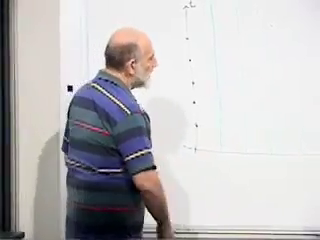
\includegraphics[width=0.62\textwidth]{lecture_01_figure_02.png}
\caption{Ось времени системы покоя и первые мировые линии пространственной решётки.}
\lectureframe{00:16:38}
\end{figure}

Та же конструкция яснее видна на идеализированном рисунке:

\begin{figure}[H]
\centering
\begin{tikzpicture}[scale=0.95]
\draw[->] (-1.2,0) -- (5.2,0) node[right] {$x$};
\draw[->] (0,-0.2) -- (0,4.8) node[above] {$t$};
\foreach \x in {-1,1,2,3,4}
  \draw[gray!65] (\x,0) -- (\x,4.4);
\foreach \y in {1,2,3,4}
  \draw[gray!65] (-1.0,\y) -- (4.4,\y);
\fill (0,0) circle (1.5pt);
\node[below left] at (0,0) {$0$};
\node[left] at (0,1) {$1$};
\node[left] at (0,2) {$2$};
\node[left] at (0,3) {$3$};
\node[below] at (1,0) {$1$};
\node[below] at (2,0) {$2$};
\node[below] at (3,0) {$3$};
\end{tikzpicture}
\caption{Неподвижная пространственно-временная решётка. Вертикальные линии соответствуют постоянному положению; горизонтальные линии — постоянному времени.}
\end{figure}

Сетка воображаемая, и её шаг произволен. Мы можем использовать метры, сантиметры, микроны или любой ещё меньший интервал, имеющий физический смысл. Её назначение — приписать точную координату каждому событию.

Теперь выражение «система отсчёта» приобретает операциональный смысл. Это не просто точка зрения и не человек, смотрящий в каком-то направлении. Это протяжённый координатный аппарат. Для данного события локальные стержни задают, где оно произошло, а локальные часы — когда. Затем между системами отсчёта можно сравнивать и другие физические величины: положение и скорость частицы, её энергию, возможно, температуру тела, а в дальнейшем — её импульс и силу. Простейшее сравнение — то, которое включает \(x\) и \(t\), поэтому с него и начнём.

Теперь поместим вторую решётку в поезд, движущийся в положительном направлении \(x\) с постоянной скоростью \(v\). Выберем начала координат так, чтобы при \(t=0\) они совпадали. Тогда движущееся начало описывается соотношением
\begin{equation}
x=vt.
\end{equation}
Любая другая точка, закреплённая в поезде, описывает параллельную наклонную мировую линию. Этот наклон — просто геометрическое выражение того, что с течением времени поезд меняет положение.

Предположим, что задняя точка поезда служит штрихованным началом координат. При \(t=0\) она совпадает с началом координат станции. В более поздний момент \(t\) её координата в неподвижной системе равна \(vt\). Поэтому близкое событие с координатой \(x\) находится от начала координат поезда всего на расстоянии \(x-vt\). Вот почему преобразование содержит вычитание, а не является произвольным алгебраическим правилом.

Пусть \((x,t)\) — координаты события в системе отсчёта станции, а \((x',t')\) — его координаты в системе отсчёта поезда. У Галилея и Ньютона время остаётся универсальным,
\begin{equation}
t'=t.
\end{equation}
За время \(t\) движущееся начало координат смещается на \(vt\), так что расстояние от него до события равно
\begin{equation}
x'=x-vt.
\end{equation}
Итак,
\begin{align}
t'&=t, & x'&=x-vt.
\label{eq:galilean-forward}
\end{align}
Решая относительно нештрихованных координат, получаем обратное преобразование,
\begin{align}
t&=t', & x&=x'+vt'.
\label{eq:galilean-inverse}
\end{align}

\begin{figure}[H]
\centering
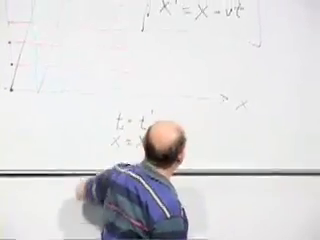
\includegraphics[width=0.72\textwidth]{lecture_01_figure_03.png}
\caption{Преобразование Галилея, записанное рядом с двумя пространственно-временными решётками.}
\lectureframe{00:21:57}
\end{figure}

Первая пара показывает движущемуся наблюдателю, как перевести координаты, заданные неподвижным наблюдателем. Обратная пара переводит обратно. Это взаимное преобразование между описаниями и составляет математическое содержание галилеевой относительности.

Замена \(t\to t'\) в обратной пространственной формуле безвредна только потому, что теория Галилея уже провозгласила \(t=t'\). Полезно отметить это предположение уже сейчас. В теории Эйнштейна эти две временные координаты будут различаться, и такие подстановки уже не будут автоматическими.

\begin{classroomqa}
\audiencequestion{Если часы унести, а потом вернуть обратно, как мы можем знать, что их движение сначала не ускорило их ход, а затем не замедлило его, скрыв эффект при сравнении часов?
\lecturetimestamp{00:23:09}}
\lecturerresponse{Галилей не мог установить универсальное время с современной точностью; это было физическое предположение. Мы можем проверять его многими способами: переносить хорошие часы в противоположных направлениях, повторять путь как по линии север--юг, так и по линии восток--запад, перемещать одни часы вокруг других или обмениваться временными сигналами, не сводя часы вместе. При обычных скоростях все такие проверки согласуются с очень высокой точностью. При достаточно точных часах или достаточно больших скоростях всё же появляется небольшое расхождение. Этот отказ универсального времени не является дефектом эксперимента; это одно из явлений, которые специальная теория относительности должна объяснить.}
\end{classroomqa}

\section{Галилеевы инварианты и закон Ньютона}

Инвариант — это величина, значение которой одинаково для всех рассматриваемых инерциальных наблюдателей. Сами координаты не обязаны быть инвариантными. Важно, сохраняют ли составленные из них законы одну и ту же форму.

Это слово употребляется и как существительное, и как прилагательное. Число может быть инвариантом, а уравнение может быть инвариантным относительно преобразования. Различие между инвариантными величинами и инвариантными законами предотвращает распространённую путаницу: теория относительности не утверждает, что каждый наблюдатель получает одну и ту же координату для всего. Она утверждает, что физический закон, связывающий их измерения, имеет одну и ту же форму.

Рассмотрим два одновременных события в положениях \(x_1\) и \(x_2\). Уравнение~\eqref{eq:galilean-forward} даёт
\begin{align}
x_1'&=x_1-vt,\\
x_2'&=x_2-vt.
\end{align}
Следовательно, расстояние между ними равно
\begin{equation}
x_2'-x_1'=(x_2-vt)-(x_1-vt)=x_2-x_1.
\end{equation}
В галилеевой физике расстояние между событиями, происходящими в одно и то же время, является инвариантом, хотя отдельные положения таковыми не являются.

\begin{classroomqa}
\audiencequestion{Действительно ли два вхождения \(t\) в этом вычитании относятся к одному и тому же времени?
\lecturetimestamp{00:28:16}}
\lecturerresponse{Да. Мы намеренно выбрали два события \((x_1,t)\) и \((x_2,t)\). Они лежат на одной горизонтальной линии постоянного времени. Поэтому общий член \(vt\) сокращается. Если бы события произошли в разные моменты времени, этот аргумент не устанавливал бы инвариантное пространственное расстояние.}
\end{classroomqa}

Теперь опишем частицу траекторией \(x(t)\). Наблюдатель в поезде приписывает
\begin{equation}
x'(t)=x(t)-vt.
\end{equation}
Дифференцируя один раз, получаем знакомое правило сложения скоростей,
\begin{equation}
\frac{dx'}{dt}=\frac{dx}{dt}-v.
\end{equation}
Положение и скорость зависят от системы отсчета. Наблюдатель, движущийся рядом со стрелой, видит, что она летит медленнее, чем наблюдатель, стоящий у путей.

Продифференцируем еще раз. Поскольку относительная скорость \(v\) постоянна,
\begin{equation}
\frac{d^2x'}{dt^2}=\frac{d^2x}{dt^2}.
\end{equation}
Ускорение инвариантно при преобразовании Галилея. Это ясно подсказывает, почему закон Ньютона записывается в терминах ускорения, а не положения или скорости.

Это ускорение наблюдаемого объекта, а не ускорение наблюдателя в поезде. Обе системы отсчета инерциальны, поэтому ни одна из них не ускоряется относительно другой. Объекты могут ускоряться влево или вправо в любом из этих описаний, и оба наблюдателя согласны относительно значения этого ускорения, хотя не согласны в положении и скорости объекта.

Предположим, что две частицы действуют друг на друга силой и эта сила зависит только от расстояния между ними в один и тот же момент времени. Это расстояние инвариантно, следовательно, инвариантна и сила. Если масса тоже является внутренним свойством, не зависящим от системы отсчета, то каждый инерциальный наблюдатель может записать
\begin{equation}
F=ma
\end{equation}
в точности в одной и той же форме. Ньютоновская механика инвариантна при преобразованиях Галилея. Это не просто правдоподобно; во всей области обычных скоростей она необычайно точна.

Этот аргумент применим к знакомым центральным силам, таким как ньютоновское тяготение или электростатика, где модуль силы является функцией расстояния. Поскольку все наблюдатели, связанные преобразованиями Галилея, согласны относительно этого расстояния в один и тот же момент времени, они согласны и относительно силы. При фиксированных силе и ускорении согласованность затем требует, чтобы они согласились и относительно массы: объект массой один килограмм остается таким же, когда его провозят мимо на поезде. Каждый символ в \(F=ma\) вписывается в одну и ту же инвариантную структуру.

\section{Свет не согласуется с галилеевским правилом}

Трудность создает электромагнетизм. Уравнения Максвелла предсказывают волны, распространяющиеся в пустом пространстве с определенной скоростью \(c\). Если уравнения Максвелла — это законы природы и законы природы одинаковы во всех инерциальных системах отсчета, то все инерциальные наблюдатели должны получать одно и то же \(c\).

Галилеева кинематика предсказывает другое. Для светового импульса, движущегося вправо в неподвижной системе отсчета, выполняется
\begin{equation}
x=ct.
\end{equation}
Применяя пространственное преобразование, получаем
\begin{equation}
x'=x-vt=(c-v)t.
\end{equation}
Поскольку \(t'=t\), наблюдатель в поезде измерил бы скорость \(c-v\).

Противоречие можно сформулировать предельно ясно. Если уравнения Максвелла сохраняют свою форму, они предсказывают \(c\) в штрихованной системе отсчета. Если сохраняется преобразование Галилея, оно предсказывает \(c-v\). Оба утверждения не могут быть точными при \(v\ne0\).

Этот результат выглядит совершенно естественным, если свет ведет себя как обычная волна в среде. Лодка, движущаяся вместе с водяной волной, измеряет меньшую относительную скорость волны. Слушатель, движущийся в неподвижном воздухе, измеряет скорость звука, смещенную движением слушателя относительно воздуха. Поэтому физики девятнадцатого века пришли к идее привилегированного состояния покоя, эфирной системы отсчета, в которой уравнения Максвелла имели бы простейшую форму, а свет двигался бы со скоростью \(c\). Эксперименты, предназначенные для обнаружения движения относительно такой привилегированной системы, не нашли никакого соответствующего эффекта.

Существовало несколько возможных экспериментальных схем, но их общая цель состояла в том, чтобы сравнить распространение света для наблюдателей, находящихся в разных состояниях движения или движущихся в разных направлениях. Ни одна не обнаружила ожидаемого галилеевского сдвига. Этот отрицательный результат не был мелкой технической неприятностью. Он вынудил выбирать между принципом относительности, уравнениями Максвелла и унаследованными представлениями о пространстве и времени.

Эйнштейн подошел к этому конфликту более прямо. В молодости он представлял себе, что гонится за световой волной. Если бы ему удалось ее догнать, ее колеблющаяся электромагнитная структура застыла бы в пространстве, однако уравнения Максвелла не допускают такой неподвижной световой волны. Он решил считать теорию Максвелла и принцип относительности фундаментальными, а затем пересмотреть предположения, скрытые в наших координатах.

Эта реконструкция опирается на два постулата:
\begin{enumerate}
\item Законы физики имеют одинаковую форму во всех инерциальных системах отсчета.
\item Свет в вакууме имеет одну и ту же скорость \(c\) во всех инерциальных системах отсчета.
\end{enumerate}

Второй постулат не может сосуществовать с преобразованием Галилея. Должно измениться нечто более глубокое, чем правило сложения скоростей. Экономный выбор Эйнштейна состоит в том, чтобы сохранить два постулата и пересмотреть кажущееся невинным галилеево уравнение \(t'=t\).

\section{Синхронизация удаленных часов}

Пространственные расстояния можно откладывать стержнями, но для удаленных часов требуется соглашение о синхронизации. Поместите двое часов на равных расстояниях от наблюдателя, находящегося посередине. Когда каждые из двух крайних часов покажут назначенное время, пусть они испустят вспышку. Если обе вспышки достигнут середины одновременно, считайте крайние часы синхронизированными. Если одна вспышка приходит первой, подстройте соответствующие часы и повторите процедуру.

Слово \emph{середина} определяется с помощью стержней, уже размещенных в данной системе отсчета. Поэтому эта проверка содержит две отдельные составляющие: одинаковое пространственное расстояние до концов и одинаковое время прихода сигналов. Нельзя отбросить ни одну из них. Повторение процедуры по всей решетке задает горизонтальные линии постоянного времени, которые Ньютон просто предполагал.

В этом определении используется свет, потому что постулат приписывает свету одну и ту же скорость в каждой инерциальной системе отсчета. После того как таким образом рассмотрены все соседние пары, на всей решетке имеется синхронизированное семейство часов.

Теперь пусть вторая решетка движется сквозь первую. В собственной системе отсчета середина движущегося устройства остается ровно посередине между двумя своими движущимися концами. Однако относительно неподвижного устройства она движется навстречу одной приближающейся вспышке и удаляется от другой. Вспышки, испущенные одновременно по неподвижным часам, не приходят вместе в движущуюся середину. Поскольку движущийся наблюдатель применяет то же правило середины и света, он не может назвать одновременными эти акты испускания. Каждая система отсчета согласованно синхронизирует свои собственные часы, но эти две синхронизации не совпадают.

Это не оптическая иллюзия, порожденная конечным временем распространения света. Каждый наблюдатель знает, что свету нужно время, чтобы прийти, и вносит поправку на это, используя одну и ту же скорость \(c\). Расхождение сохраняется и после этой поправки, потому что наблюдатели не выбирают одну и ту же пару удаленных событий как одновременную. Относительна сама одновременность, а не только видимость одновременности.

\begin{classroomqa}
\audiencequestion{Могли бы мы избежать этого вывода, синхронизируя часы звуком вместо света?
\lecturetimestamp{00:49:03}}
\lecturerresponse{Звук годится как сигнал синхронизации в системе отсчета, где воздух покоится, но его измеренная скорость не одинакова во всех инерциальных системах отсчета. Открытый поезд, движущийся сквозь неподвижный воздух, движется относительно среды, переносящей звук, поэтому звуковые сигналы вперед и назад ведут себя там несимметрично. Со светом по постулату иначе: не существует обнаружимой оптической среды, чья система покоя выделяла бы одного наблюдателя. Поэтому мы используем свет и прослеживаем последствия.}
\end{classroomqa}

Качественное расхождение ясно. Теперь мы точно вычислим, какие события движущийся наблюдатель считает одновременными.

\section{Построение с помощью световых лучей}

Для этого построения удобно выбрать единицы, в которых
\begin{equation}
c=1.
\end{equation}
Тогда единица расстояния — это расстояние, которое свет проходит за единицу времени: световые секунды в паре с секундами или световые годы в паре с годами. Пространство и время имеют одни и те же единицы, скорости безразмерны, а световые лучи изображаются под углом \(45^\circ\). Для луча, идущего вправо,
\begin{equation}
x=t+d,
\end{equation}
а для луча, идущего влево,
\begin{equation}
x=-t+d'.
\end{equation}
Два луча, проходящие через начало координат, — это просто \(x=t\) и \(x=-t\). Времеподобные траектории, соответствующие объектам медленнее света, лежат ближе к вертикальной оси. Гипотетическая сверхсветовая траектория лежала бы ближе к горизонтальной оси.

Угол на рисунке имеет смысл только после такого выбора единиц. В метрах и секундах световой луч выглядел бы почти горизонтальным, потому что за одну секунду он проходит примерно \(3\times10^8\) метров. Выбор световых секунд в качестве единицы расстояния меняет масштаб горизонтальной оси и делает причинную геометрию видимой.

Рассмотрим три параллельные мировые линии в движущейся решётке,
\begin{equation}
x=vt,\qquad x=vt+L,\qquad x=vt+2L.
\label{eq:moving-worldlines}
\end{equation}
Средняя мировая линия принадлежит наблюдателю, который проверяет одновременность между двумя крайними точками. Все три точки движутся равномерно и сохраняют своё взаимное расположение в штрихованной системе отсчёта.

\begin{figure}[H]
\centering
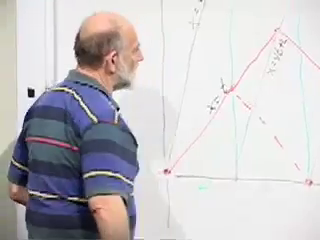
\includegraphics[width=0.72\textwidth]{lecture_01_figure_04.png}
\caption{Световой луч \(x=t\), идущий вправо, пересекает среднюю движущуюся мировую линию.}
\lectureframe{01:02:33}
\end{figure}

Полную геометрию можно изобразить без помехи со стороны человека, стоящего у доски:

\begin{figure}[H]
\centering
\begin{tikzpicture}[scale=0.95]
\draw[->] (-0.5,0) -- (6.5,0) node[right] {$x$};
\draw[->] (0,-0.2) -- (0,4.3) node[above] {$t$};
\draw[blue] (0,0) -- (1.4,4.0);
\draw[blue] (2.0,0) -- (3.4,4.0);
\draw[blue] (4.0,0) -- (5.4,4.0);
\draw[red] (0,0) -- (3.08,3.08);
\draw[red] (3.08,3.08) -- (4.56,1.60);
\draw[red,dashed] (2.0,0) -- (4.56,1.60);
\fill (0,0) circle (1.5pt);
\fill (2.0,0) circle (1.5pt);
\fill (4.0,0) circle (1.5pt);
\fill (3.08,3.08) circle (1.5pt);
\fill (4.56,1.60) circle (1.5pt);
\node[left] at (0.55,1.55) {$x=vt$};
\node[left] at (2.45,1.9) {$x=vt+L$};
\node[right] at (4.72,1.9) {$x=vt+2L$};
\node[left] at (1.88,2.28) {$x=t$};
\node[above right] at (3.08,3.08) {$A$};
\end{tikzpicture}
\caption{Световые сигналы определяют линию одновременности движущейся системы отсчёта.}
\end{figure}

Пустим из начала координат световой луч, идущий вправо. Пусть \(A\) — точка его пересечения со средней мировой линией. В точке \(A\) выполняются два уравнения
\begin{align}
x&=t,\\
x&=vt+L.
\end{align}
Подстановка даёт
\begin{equation}
t=vt+L,
\end{equation}
и, следовательно,
\begin{equation}
t_A=x_A=\frac{L}{1-v}.
\label{eq:point-a}
\end{equation}

Из \(A\) проследим назад световой луч, идущий влево, до самой правой движущейся мировой линии. Его уравнение имеет вид
\begin{equation}
x+t=b.
\end{equation}
Поскольку он проходит через \(A\), уравнение~\eqref{eq:point-a} определяет константу:
\begin{equation}
b=x_A+t_A=\frac{2L}{1-v}.
\end{equation}
Следовательно, для этого луча выполняется
\begin{equation}
x+t=\frac{2L}{1-v}.
\label{eq:backward-ray}
\end{equation}

Его пересечение с самой правой мировой линией определяется из
\begin{align}
x+t&=\frac{2L}{1-v},\\
x&=vt+2L.
\end{align}
Исключая \(x\),
\begin{align}
(1+v)t
  &=2L\left(\frac{1}{1-v}-1\right)\\
  &=\frac{2Lv}{1-v},
\end{align}
откуда
\begin{equation}
t=\frac{2Lv}{1-v^2}.
\end{equation}
Подстановка в \(x=vt+2L\) даёт
\begin{equation}
x=\frac{2L}{1-v^2}.
\end{equation}
Сами координаты менее важны, чем их отношение:
\begin{equation}
\frac{t}{x}=v.
\end{equation}
Итак, каждое событие, одновременное с началом координат по часам движущейся системы, лежит на прямой
\begin{equation}
t=vx,
\label{eq:simultaneity-c-one}
\end{equation}
тогда как мировая линия движущегося начала координат задаётся уравнением
\begin{equation}
x=vt.
\label{eq:moving-time-axis}
\end{equation}
Обе оси наклонены симметрично относительно светового луча, идущего под углом \(45^\circ\).

Все точки на \(x=vt\) имеют одну и ту же штрихованную пространственную координату, \(x'=0\), тогда как их штрихованные времена различаются. Все точки на \(t=vx\) имеют одно и то же штрихованное время, \(t'=0\), тогда как их штрихованные пространственные координаты различаются. Следовательно, одна из этих прямых является штрихованной осью времени, а другая — штрихованной пространственной осью. Длинное построение со световыми сигналами понадобилось для определения второй прямой; вывести её только из движущейся мировой линии было нельзя.

Для восстановления обычных единиц в уравнении~\eqref{eq:simultaneity-c-one} требуется
\begin{equation}
t=\frac{v}{c^2}x.
\label{eq:simultaneity-dimensional}
\end{equation}
Множитель \(c^2\) объясняет, почему ньютоновская картина так хорошо работает в повседневной жизни. Для скоростей, очень малых по сравнению с \(c\), наклон линии одновременности движущейся системы чрезвычайно мал.

\begin{figure}[H]
\centering
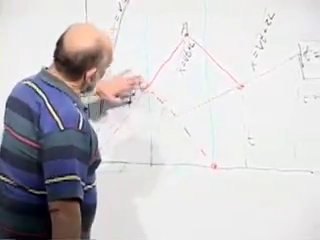
\includegraphics[width=0.72\textwidth]{lecture_01_figure_05.png}
\caption{При \(c=1\) штрихованная ось времени и ось одновременности симметричны относительно светового луча.}
\lectureframe{01:15:40}
\end{figure}

\begin{figure}[H]
\centering
\begin{tikzpicture}[scale=1.0]
\draw[->] (-2.2,0) -- (5.2,0) node[right] {$x$};
\draw[->] (0,-0.2) -- (0,4.9) node[above] {$t$};
\draw[red] (0,0) -- (3.9,3.9);
\draw[red] (0,0) -- (-1.8,1.8);
\draw[blue] (0,0) -- (1.8,4.5);
\draw[blue,dashed] (0,0) -- (4.5,1.8);
\node[right] at (3.9,3.9) {$x=t$};
\node[left] at (-1.8,1.8) {$x=-t$};
\node[above] at (1.8,4.5) {$x'=0$};
\node[right] at (4.5,1.8) {$t'=0$};
\end{tikzpicture}
\caption{Штрихованные оси и инвариантные световые лучи в единицах \(c=1\).}
\end{figure}

\section{Вывод преобразования Лоренца}

Геометрия задаёт, где обращается в нуль каждая штрихованная координата. Вдоль движущейся оси времени \(x=vt\) должно быть \(x'=0\). Вдоль движущейся оси одновременности \(t=vx\) должно быть \(t'=0\). Самые общие линейные соотношения, обращающиеся в нуль именно на этих прямых, можно записать в виде
\begin{align}
x'&=\frac{x-vt}{F(v)},\\
t'&=\frac{t-vx}{G(v)}.
\label{eq:fg-ansatz}
\end{align}
Множители \(F\) и \(G\) допускают, что масштабы штрихованных координат отличаются от галилеевых масштабов, хотя сами оси уже определены. Линейность следует из однородности пространства и времени: перенос эксперимента не может изменить закон преобразования.\editorialnote{Этот краткий довод о линейности делает явным предположение, неявно использованное в выводе у доски.}

На этом этапе геометрия сказала нам многое, но не всё. Числители фиксируют наклон осей. Они не фиксируют расстояние между делениями единичной шкалы вдоль этих осей. Именно эту оставшуюся информацию о масштабе и представляют \(F(v)\) и \(G(v)\).

Теперь наложим условие инвариантности скорости света. Световой луч, идущий вправо и подчиняющийся \(x=t\), должен также подчиняться \(x'=t'\). Вдоль этого луча,
\begin{align}
x'&=\frac{(1-v)t}{F(v)},\\
t'&=\frac{(1-v)t}{G(v)}.
\end{align}
Чтобы равенство выполнялось для каждой точки на луче, необходимо
\begin{equation}
F(v)=G(v).
\end{equation}
Поэтому можно записать
\begin{align}
x'&=\frac{x-vt}{F(v)},\\
t'&=\frac{t-vx}{F(v)}.
\label{eq:common-f}
\end{align}

На этом шаге в алгебре впервые используется по-настоящему эйнштейновское требование. Одна и та же геометрическая прямая является световым лучом для обоих наблюдателей, поэтому при \(c=1\) обе штрихованные координаты должны изменяться вдоль неё одинаково. Разные множители в двух уравнениях привели бы к тому, что штрихованная скорость отличалась бы от единицы.

Остаётся одна неизвестная функция. Умножим уравнение~\eqref{eq:common-f} на \(F(v)\):
\begin{align}
F(v)x'&=x-vt,\\
F(v)t'&=t-vx.
\end{align}
Умножая второе уравнение на \(v\) и прибавляя его к первому, исключаем \(t\) и получаем
\begin{equation}
(1-v^2)x=F(v)(x'+vt').
\end{equation}
Аналогично,
\begin{equation}
(1-v^2)t=F(v)(t'+vx').
\end{equation}
Следовательно, обратное преобразование имеет вид
\begin{align}
x&=\frac{F(v)}{1-v^2}(x'+vt'),\\
t&=\frac{F(v)}{1-v^2}(t'+vx').
\end{align}

Принцип относительности делает две системы взаимными. Если станция видит, что поезд движется со скоростью \(+v\), то поезд видит, что станция движется со скоростью \(-v\). Поэтому обратные уравнения должны иметь тот же вид, что и прямые, но с обратным знаком у \(v\). Их предмножители должны удовлетворять условию
\begin{equation}
\frac{F(v)}{1-v^2}=\frac{1}{F(v)}.
\end{equation}
Отсюда
\begin{equation}
F(v)^2=1-v^2,
\end{equation}
а непрерывность при переходе к тождественному преобразованию при \(v=0\) выбирает положительный корень,
\begin{equation}
F(v)=\sqrt{1-v^2}.
\end{equation}

Ничего не подгонялось под какой-то конкретный световой импульс. Результат следует из осей, зафиксированных синхронизацией, общей скорости света и требования, чтобы ни одна из двух инерциальных систем не была привилегированной по отношению к другой.

Преобразование Лоренца в единицах, где \(c=1\), имеет вид
\begin{align}
x'&=\frac{x-vt}{\sqrt{1-v^2}},\\
t'&=\frac{t-vx}{\sqrt{1-v^2}}.
\label{eq:lorentz-c-one}
\end{align}
Его обратное преобразование имеет вид
\begin{align}
x&=\frac{x'+vt'}{\sqrt{1-v^2}},\\
t&=\frac{t'+vx'}{\sqrt{1-v^2}}.
\end{align}

\begin{figure}[H]
\centering
\includegraphics[width=0.76\textwidth]{lecture_01_figure_06.png}
\caption{Окончательный вид преобразования Лоренца при \(c=1\) на доске.}
\lectureframe{01:32:38}
\end{figure}

Существенная новизна уже видна в уравнении для времени. При переходе от одной системы отсчёта к другой время не остаётся просто неизменным. Штрихованная временная координата смешивает нештрихованные время и пространственную координату. Следовательно, \(t=\text{constant}\) и \(t'=\text{constant}\) описывают разные множества событий.

Смешивающий член — не факультативная поправка, добавляемая задним числом. Без него прямая \(t'=0\) оставалась бы горизонтальной, удалённая одновременность оставалась бы универсальной, и преобразование не могло бы сохранять скорость света.

\section{Восстановление скорости света и проверка результата}

Когда \(c\ne1\), размерностная согласованность восстанавливает недостающие множители. Отношение \(v^2/c^2\) безразмерно, тогда как \((v/c^2)x\) имеет размерность времени. Поэтому
\begin{align}
x'&=\frac{x-vt}{\sqrt{1-v^2/c^2}},\\
t'&=\frac{t-(v/c^2)x}{\sqrt{1-v^2/c^2}}.
\label{eq:lorentz-dimensional}
\end{align}
Обратное преобразование получается обращением знака у \(v\):
\begin{align}
x&=\frac{x'+vt'}{\sqrt{1-v^2/c^2}},\\
t&=\frac{t'+(v/c^2)x'}{\sqrt{1-v^2/c^2}}.
\end{align}
Введение
\begin{equation}
\gamma=\frac{1}{\sqrt{1-v^2/c^2}}
\end{equation}
привело бы эти выражения к привычному компактному виду, но запись со знаменателем позволяет видеть сам вывод.

Численно \(c\simeq3\times10^8\,\mathrm{m/s}\), так что \(c^2\simeq9\times10^{16}\,\mathrm{m^2/s^2}\). Большой знаменатель делает и наклон линии одновременности, и множитель \(v^2/c^2\) незаметными в большинстве механических экспериментов. Их малость объясняет успех Галилея, но не восстанавливает абсолютное время.

\begin{figure}[H]
\centering
\includegraphics[width=0.76\textwidth]{lecture_01_figure_07.png}
\caption{Преобразование Лоренца после восстановления множителей \(c\).}
\lectureframe{01:35:58}
\end{figure}

Сразу можно выполнить две проверки. Сначала возьмём \(v\ll c\). Тогда \(v^2/c^2\) пренебрежимо мало, и для обычных расстояний член относительности одновременности \(vx/c^2\) тоже пренебрежимо мал. Уравнение~\eqref{eq:lorentz-dimensional} сводится к виду
\begin{equation}
t'\approx t,\qquad x'\approx x-vt.
\end{equation}
Галилеева относительность восстанавливается как приближение малых скоростей.

Во-вторых, проверим световой луч. После восстановления \(c\) луч, идущий вправо, подчиняется \(x=ct\), а не \(x=t\). Подстановка даёт
\begin{align}
x'&=\frac{(c-v)t}{\sqrt{1-v^2/c^2}},\\
t'&=\frac{(1-v/c)t}{\sqrt{1-v^2/c^2}}.
\end{align}
Поскольку \(c-v=c(1-v/c)\),
\begin{equation}
x'=ct'.
\end{equation}
Наблюдатель в штрихованной системе измеряет ту же скорость \(c\). Для луча, идущего влево, подстановка \(x=-ct\) аналогично даёт
\begin{equation}
x'=-ct'.
\end{equation}
Преобразование правильно описывает свет, движущийся в любом направлении.

Различие между \(x=t\) и \(x=ct\) служит поучительной размерностной проверкой. Первое равенство верно только в единицах, где \(c=1\). Если восстановить обычные единицы в преобразовании, но оставить уравнение луча в естественных единицах, то это смешает две конвенции и даст ложный результат. Размерностная согласованность немедленно обнаруживает ошибку.

\section{Критерий середины}

\begin{classroomqa}
\audiencequestion{Предположим, что наблюдатель получает две вспышки в один и тот же момент, но сам не находится посередине между их источниками. Может ли он заключить, что вспышки были испущены одновременно?
\lecturetimestamp{01:42:55}}
\lecturerresponse{Нет. Равенство времён прихода влечёт равенство времён испускания только для того наблюдателя, который в соответствующей системе отсчёта находится посередине между двумя источниками. Приёмник, расположенный ближе к одному источнику, может получить обе вспышки одновременно, даже если более далёкая была испущена раньше. Поэтому в движущейся конструкции мировая линия середины \(x=vt+L\) существенна. Луч \(x=t\) прослеживается до встречи с этой серединой, а затем назад проводится световой луч к \(x=vt+2L\). Именно событие в этой второй конечной точке, а не произвольное событие равного прихода где-либо ещё, является одновременным с началом координат согласно движущейся системе.}
\end{classroomqa}

Мы получили полное координатное преобразование, но ещё не дошли до его наиболее привычных следствий. Далее следуют сокращение длины, замедление времени и собственное время, а затем релятивистские импульс и энергия. Основание уже заложено: каждая инерциальная система может использовать одни и те же законы и измерять одну и ту же скорость света только потому, что пространство и время смешиваются и что удалённая одновременность принадлежит системе отсчёта, а не миру как таковому.

\chapter{Уравнения Максвелла, ковариантность и электромагнитные волны}

\lectureoverview{Электрическое и магнитное поля действуют на заряженное вещество через силу Лоренца, но вещество должно также создавать поля и изменять их конфигурацию. Мы сформулируем эту обратную половину электромагнетизма, покажем, что уравнения Максвелла лоренц-ковариантны, выведем их волновые решения, а затем вернём заряд и ток в форме, которая делает локальный закон сохранения явным. На протяжении всей лекции мы используем единицы, в которых \(c=1\).}

\section{Другая половина электромагнетизма}

Начнём с той части предмета, которая уже нам известна. Если частица с зарядом \(q\) движется со скоростью \(\mathbf v\) в электрическом и магнитном полях, то сила равна
\begin{equation}
\mathbf F=q\bigl(\mathbf E+\mathbf v\times\mathbf B\bigr).
\label{eq:lorentz-force-three}
\end{equation}
Множитель \(q\) принципиально необходим. Незаряженная частица не испытывает электромагнитной силы. Электрическое поле даёт вклад даже тогда, когда частица мгновенно покоится, тогда как магнитный вклад зависит от её движения.

Уравнение~\eqref{eq:lorentz-force-three} говорит нам, что делают с веществом заданные поля. Оно не говорит, чем определяются сами поля. Что создаёт электрическое поле вокруг одного объекта, магнитное поле вокруг другого или волну, движущуюся через пустое пространство? На эти вопросы отвечают уравнения Максвелла.

\begin{figure}[H]
\centering
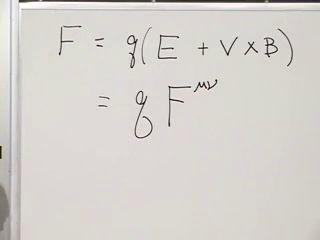
\includegraphics[width=0.62\textwidth]{lecture_58_figure_02.png}
\caption{Трёхвекторная сила Лоренца и начало её тензорной переформулировки.}
\lectureframe{00:05:49}
\end{figure}

Релятивистская форма закона силы предвосхищает обозначения, которые нам понадобятся:
\begin{equation}
f^\mu=qF^\mu{}_{\nu}u^\nu.
\label{eq:lorentz-force-four}
\end{equation}
Здесь \(u^\nu\) — это четырёхскорость, \(f^\mu\) — четырёхсила, а \(F^{\mu\nu}\) — антисимметричный тензор, составленный из \(\mathbf E\) и \(\mathbf B\). На доске сначала показано лишь схематическое начало этого выражения; свёртка с \(u^\nu\) даёт недостающий вектор, необходимый, чтобы остался один свободный индекс силы.

Есть физическая причина, по которой вещество должно воздействовать обратно на поле. Электромагнитная волна может налететь на заряд, ускорить его и передать ему энергию. Если бы поле могло воздействовать на заряд, а заряд никак не мог бы воздействовать на поле, не было бы места, откуда эта энергия была бы изъята. Принцип действия и противодействия — не весь аргумент, но закон сохранения энергии делает такую взаимную связь неизбежной.

\section{Изменяющийся источник порождает возмущение}

Точечный заряд создаёт электрическое поле, направленное наружу от его положения или внутрь к нему. Ток в проводе--поток заряженных частиц--создаёт магнитное поле, циркулирующее вокруг провода. Эти знакомые статические картины уже показывают две разные геометрические структуры: электрический поток исходит от заряда, тогда как линии магнитного поля обвивают ток.

Теперь резко переместим точечный заряд. Вблизи его нового положения электрическое поле должно начать перестраиваться, но далёкий наблюдатель не может узнать об этом движении мгновенно. Вдали старое поле сохраняется до тех пор, пока сигнал не успеет прийти. Между ближней и дальней областями находится движущийся фронт, на котором поле изменяется. Эта движущаяся перестройка и есть электромагнитное возмущение.

Если заряд заставить двигаться туда и обратно, последовательные перестройки будут следовать одна за другой и образуют электромагнитную волну. В этом и состоит элементарная функция антенны: колеблющийся электрический ток посылает наружу возмущение поля. Обращение тока в проводе даёт магнитный вариант того же рассуждения. Циркуляция \(\mathbf B\) должна обратиться, но это обращение распространяется, а не возникает сразу повсюду.

Эта причинная картина ставит перед уравнениями Максвелла две задачи. Они должны описывать, как заряд и ток служат источниками полей, и должны допускать распространение изменений в этих полях не быстрее света. Вторая задача одновременно является и проверкой теории относительности. Если уравнения Максвелла имеют один и тот же вид в каждой инерциальной системе отсчёта и влекут определённую скорость волны, то каждая инерциальная система должна выводить из них одну и ту же скорость.

\section{Повторение релятивистского волнового уравнения}

Прежде чем переходить к векторным полям, рассмотрим скалярное поле \(\phi(\mathbf x,t)\), одно число в каждой точке пространства-времени. Уравнение с первыми производными
\begin{equation}
\partial_\mu\phi=0
\end{equation}
означало бы, что все производные по координатам пространства-времени равны нулю. Поле было бы постоянным и потому не могло бы нести волну. Нетривиальное релятивистское волновое уравнение использует две производные:
\begin{equation}
\partial_\mu\partial^\mu\phi=0.
\end{equation}
При используемом здесь соглашении о знаках
\begin{equation}
\left(\partial_t^2-\partial_x^2-\partial_y^2-\partial_z^2\right)\phi=0,
\label{eq:scalar-wave-four}
\end{equation}
или, более компактно,
\begin{equation}
\left(\partial_t^2-\nabla^2\right)\phi=0.
\end{equation}
Выбор \(c=1\) делает единицы времени и расстояния согласованными. При восстановлении обычных единиц множитель \(1/c^2\) появился бы при второй производной по времени.

Для волны, распространяющейся вдоль оси \(z\), поле зависит от \(z\) и \(t\), а не от \(x\) или \(y\). Уравнение~\eqref{eq:scalar-wave-four} принимает вид
\begin{equation}
\left(\partial_t^2-\partial_z^2\right)\phi=0.
\label{eq:scalar-wave-one}
\end{equation}

\begin{figure}[H]
\centering
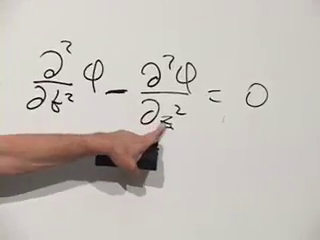
\includegraphics[width=0.56\textwidth]{lecture_58_figure_04.png}
\caption{Одномерное скалярное волновое уравнение, используемое в качестве модели для электромагнитных волн.}
\lectureframe{00:47:03}
\end{figure}

Его общий вид бегущей волны таков:
\begin{equation}
\phi(z,t)=f(z-t)+g(z+t).
\end{equation}
Профиль \(f(z-t)\) движется в сторону возрастания \(z\), поскольку точка фиксированной фазы удовлетворяет \(z-t=\text{constant}\). Профиль \(g(z+t)\) движется в противоположном направлении. Ничто не требует, чтобы какой-либо из этих профилей был синусоидальным; любая достаточно гладкая форма распространяется без изменения формы.

Синусоиды, однако, удобны:
\begin{equation}
\phi(z,t)=A\cos\!\bigl(k(z-t)\bigr).
\end{equation}
Волновое число \(k\) определяет длину волны,
\begin{equation}
\lambda=\frac{2\pi}{k}.
\end{equation}
Большое \(k\) даёт быстрые пространственные осцилляции и малую длину волны; малое \(k\) даёт большую длину волны. Эти же профили вскоре станут компонентами \(\mathbf E\) и \(\mathbf B\).

\section{Векторный анализ, необходимый для уравнений Максвелла}

Уравнения Максвелла записываются с помощью скалярных произведений, векторных произведений, дивергенции и ротора. Стоит один раз заново восстановить эти обозначения, потому что последующие покомпонентные вычисления используют именно такие структуры.

Для обычных трёхмерных векторов \(\mathbf a\) и \(\mathbf b\) скалярное произведение есть скаляр
\begin{equation}
\mathbf a\cdot\mathbf b
=a_xb_x+a_yb_y+a_zb_z.
\end{equation}
Векторное произведение — ещё один вектор,
\begin{align}
(\mathbf a\times\mathbf b)_x&=a_yb_z-a_zb_y,\\
(\mathbf a\times\mathbf b)_y&=a_zb_x-a_xb_z,\\
(\mathbf a\times\mathbf b)_z&=a_xb_y-a_yb_x.
\end{align}
Остальные компоненты следуют из циклического порядка \(x\to y\to z\to x\).

Введём дифференциальный оператор
\begin{equation}
\boldsymbol\nabla=
\left(\partial_x,\partial_y,\partial_z\right).
\end{equation}
Его компоненты являются операторами, а не обычными числами, но схемы скалярного и векторного произведений всё равно можно использовать. Для векторного поля \(\mathbf A\)
\begin{equation}
\boldsymbol\nabla\cdot\mathbf A
=\partial_xA_x+\partial_yA_y+\partial_zA_z
\label{eq:divergence}
\end{equation}
есть дивергенция, тогда как
\begin{align}
(\boldsymbol\nabla\times\mathbf A)_x
 &=\partial_yA_z-\partial_zA_y,\\
(\boldsymbol\nabla\times\mathbf A)_y
 &=\partial_zA_x-\partial_xA_z,\\
(\boldsymbol\nabla\times\mathbf A)_z
 &=\partial_xA_y-\partial_yA_x
\label{eq:curl}
\end{align}
есть компоненты ротора.

Геометрия не менее важна, чем формулы. Векторное поле имеет положительную дивергенцию там, где кажется, что оно растекается наружу от источника. Оно имеет ротор там, где циркулирует. Радиальное электрическое поле точечного заряда иллюстрирует дивергенцию; магнитное поле, обвивающее провод с током, иллюстрирует ротор. Пространственно постоянное векторное поле не имеет ни того, ни другого.

\section{Уравнения Максвелла в вакууме}

В отсутствие заряда и тока уравнения Максвелла имеют вид
\begin{align}
\boldsymbol\nabla\times\mathbf E&=-\partial_t\mathbf B,
\label{eq:faraday-vac}\\
\boldsymbol\nabla\cdot\mathbf B&=0,
\label{eq:gauss-b-vac}\\
\boldsymbol\nabla\times\mathbf B&=\partial_t\mathbf E,
\label{eq:ampere-vac}\\
\boldsymbol\nabla\cdot\mathbf E&=0.
\label{eq:gauss-e-vac}
\end{align}
Два уравнения на ротор почти переходят друг в друга при замене \(\mathbf E\) на \(\mathbf B\), но их различает существенный знак минус. Два уравнения на дивергенцию говорят, что ни одно из полей не имеет источника в рассматриваемой области вакуума. Магнитная дивергенция остаётся нулевой даже после того, как электрические источники будут возвращены; обычный электромагнетизм не содержит магнитного заряда.

\begin{figure}[H]
\centering
\includegraphics[width=0.76\textwidth]{lecture_58_figure_06.png}
\caption{Четыре вакуумных уравнения Максвелла, записанные так, чтобы показать почти симметрию между электрическим и магнитным полями.}
\lectureframe{00:27:30}
\end{figure}

Плотность заряда \(\rho\) впоследствии заменит нуль в правой части уравнения~\eqref{eq:gauss-e-vac}, а плотность тока \(\mathbf J\) войдёт в уравнение~\eqref{eq:ampere-vac}. Пока временно отложим эти члены. Уравнения без источников выявляют структуру преобразований и волновой механизм при минимуме лишних членов.

Они также делают ещё острее эйнштейновскую проблему. Наблюдатель, следующий за волной в галилеевой кинематике, ожидал бы вычесть скорости и измерить меньшую скорость волны. Однако если одни и те же уравнения Максвелла выполняются в каждой инерциальной системе отсчёта, то каждый наблюдатель выводит из них одну и ту же единичную скорость волны. Выход состоит не в том, чтобы изменять волновое уравнение от системы к системе. Он состоит в том, чтобы использовать преобразование Лоренца и выразить уравнения Максвелла через объекты, законы преобразования которых уже известны.

\section{Электрическое и магнитное поля как единый тензор}

Электрическое и магнитное поля объединяются в антисимметричный тензор поля
\begin{equation}
F^{\mu\nu}=
\begin{pmatrix}
0   & -E_x & -E_y & -E_z\\
E_x & 0    & -B_z & B_y\\
E_y & B_z  & 0    & -B_x\\
E_z & -B_y & B_x  & 0
\end{pmatrix},
\label{eq:l0203-field-tensor}
\end{equation}
где порядок строк и столбцов таков: \(t,x,y,z\). Антисимметрия,
\begin{equation}
F^{\mu\nu}=-F^{\nu\mu},
\end{equation}
заставляет диагональные элементы обращаться в нуль и определяет нижнюю половину матрицы по верхней. Временнó-пространственные элементы содержат \(\mathbf E\); чисто пространственные элементы содержат \(\mathbf B\).

\begin{figure}[H]
\centering
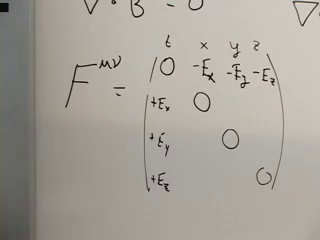
\includegraphics[width=0.58\textwidth]{lecture_58_figure_03.png}
\caption{Полный тензор электромагнитного поля, включая его электрические и магнитные компоненты.}
\lectureframe{00:32:05}
\end{figure}

Важность \(F^{\mu\nu}\) состоит не только в том, что шесть компонент поля помещаются в одну матрицу. При преобразовании Лоренца он преобразуется как тензор второго ранга. Поэтому электрические и магнитные поля, измеряемые разными наблюдателями, смешиваются ровно так, как требуется, чтобы весь объект преобразовывался согласованно.

Существует второй антисимметричный тензор — дуальный тензор поля \(\widetilde F^{\mu\nu}\). При принятой здесь конвенции он получается из уравнения~\eqref{eq:l0203-field-tensor} заменой
\begin{equation}
\mathbf E\longmapsto-\mathbf B,
\qquad
\mathbf B\longmapsto\mathbf E.
\label{eq:dual-replacement}
\end{equation}
Отсюда
\begin{equation}
\widetilde F^{\mu\nu}=
\begin{pmatrix}
0    & B_x  & B_y  & B_z\\
-B_x & 0    & -E_z & E_y\\
-B_y & E_z  & 0    & -E_x\\
-B_z & -E_y & E_x  & 0
\end{pmatrix}.
\label{eq:dual-tensor}
\end{equation}
Знак в уравнении~\eqref{eq:dual-replacement} существен. В лекции сначала пытаются выполнить эту перестановку на словах, замечают несоответствие знака и исправляют его, прежде чем завершить матрицу.

\begin{figure}[H]
\centering
\includegraphics[width=0.58\textwidth]{lecture_58_figure_07.png}
\caption{Дуальный тензор строится перестановкой электрических и магнитных компонент с требуемым знаком.}
\lectureframe{00:35:45}
\end{figure}

\section{Ковариантные уравнения в вакууме}

Каждое уравнение Максвелла содержит одну производную. Если начать с тензора ранга два и свернуть по одному индексу производной, останется один свободный индекс, поэтому естественными ковариантными кандидатами являются
\begin{align}
\partial_\mu F^{\mu\nu}&=0,
\label{eq:maxwell-covariant-vac}\\
\partial_\mu\widetilde F^{\mu\nu}&=0.
\label{eq:maxwell-dual-vac}
\end{align}
Для каждого фиксированного значения \(\nu\) уравнение~\eqref{eq:maxwell-covariant-vac} представляет собой одно уравнение. Поскольку \(\nu\) может принимать значения \(t,x,y,z\), оно объединяет четыре скалярных уравнения. Уравнение~\eqref{eq:maxwell-dual-vac} объединяет ещё четыре. Это соответствует двум векторным уравнениям на ротор и двум скалярным уравнениям на дивергенцию в исходном списке.

Компактная запись полезна лишь тогда, когда она воспроизводит знакомые уравнения. Возьмём \(\nu=z\):
\begin{align}
\partial_\mu F^{\mu z}
&=\partial_tF^{tz}
  +\partial_xF^{xz}
  +\partial_yF^{yz}
  +\partial_zF^{zz}\\
&=-\partial_tE_z+\partial_xB_y-\partial_yB_x\\
&=-\partial_tE_z+
  \bigl(\boldsymbol\nabla\times\mathbf B\bigr)_z.
\end{align}
Член \(F^{zz}\) обращается в нуль по антисимметрии. Приравнивание результата к нулю даёт \(z\)-компоненту
\begin{equation}
\boldsymbol\nabla\times\mathbf B=\partial_t\mathbf E.
\end{equation}
\(x\)- и \(y\)-компоненты получаются циклической перестановкой индексов.

\begin{figure}[H]
\centering
\includegraphics[width=0.76\textwidth]{lecture_58_figure_08.png}
\caption{Покомпонентное разложение ковариантного уравнения поля; диагональный элемент тензора обращается в нуль, а остальные члены восстанавливают уравнения Максвелла.}
\lectureframe{00:43:30}
\end{figure}

Теперь возьмём временную компоненту:
\begin{align}
\partial_\mu F^{\mu t}
&=\partial_tF^{tt}
  +\partial_xF^{xt}
  +\partial_yF^{yt}
  +\partial_zF^{zt}\\
&=\partial_xE_x+\partial_yE_y+\partial_zE_z\\
&=\boldsymbol\nabla\cdot\mathbf E.
\end{align}
Следовательно, это даёт уравнение~\eqref{eq:gauss-e-vac}. Те же проверки для дуального тензора дают
\(\boldsymbol\nabla\cdot\mathbf B=0\) и
\(\boldsymbol\nabla\times\mathbf E=-\partial_t\mathbf B\).

Компактные уравнения теперь установлены, а не просто угаданы. Их структура со свободным индексом делает их четырёхвекторными уравнениями, поэтому преобразование Лоренца меняет их компоненты, но не их форму. Именно в этом точном смысле вакуумные уравнения Максвелла одинаковы во всех инерциальных системах отсчёта.

\section{От уравнений первого порядка к волне}

Уравнения Максвелла содержат только первые производные, тогда как волновое уравнение содержит вторые производные. Кажущееся несоответствие устраняется тем, что теория Максвелла связывает два поля. Пару уравнений первого порядка для \(\mathbf E\) и \(\mathbf B\) можно объединить в уравнение второго порядка для любого из этих полей по отдельности.

Продифференцируем уравнение~\eqref{eq:ampere-vac} по времени:
\begin{equation}
\partial_t^2\mathbf E
=\boldsymbol\nabla\times\partial_t\mathbf B.
\end{equation}
Закон Фарадея даёт временную производную \(\mathbf B\),
\begin{equation}
\partial_t\mathbf B=-\boldsymbol\nabla\times\mathbf E,
\end{equation}
и потому
\begin{equation}
\partial_t^2\mathbf E
=-\boldsymbol\nabla\times
  \bigl(\boldsymbol\nabla\times\mathbf E\bigr).
\label{eq:double-curl}
\end{equation}

На доске подробно разбирается одна компонента, а не используется заученное тождество. Для \(x\)-компоненты
\begin{align}
\bigl[\boldsymbol\nabla\times
(\boldsymbol\nabla\times\mathbf E)\bigr]_x
&=\partial_y(\boldsymbol\nabla\times\mathbf E)_z
 -\partial_z(\boldsymbol\nabla\times\mathbf E)_y\\
&=\partial_y(\partial_xE_y-\partial_yE_x)\\
&\quad-\partial_z(\partial_zE_x-\partial_xE_z)\\
&=\partial_x(\partial_yE_y+\partial_zE_z)
 -\partial_y^2E_x\\
&\quad-\partial_z^2E_x.
\end{align}
Прибавим и вычтем \(\partial_x^2E_x\), чтобы выделить дивергенцию:
\begin{align}
\bigl[\boldsymbol\nabla\times
(\boldsymbol\nabla\times\mathbf E)\bigr]_x
&=\partial_x(\boldsymbol\nabla\cdot\mathbf E)
 -\nabla^2E_x.
\label{eq:double-curl-x}
\end{align}
В вакууме \(\boldsymbol\nabla\cdot\mathbf E=0\). Объединяя
уравнения~\eqref{eq:double-curl} и \eqref{eq:double-curl-x}, получаем
\begin{equation}
\left(\partial_t^2-\nabla^2\right)E_x=0.
\label{eq:ex-wave}
\end{equation}

\begin{figure}[H]
\centering
\includegraphics[width=0.72\textwidth]{lecture_58_figure_09.png}
\caption{Покомпонентный расчёт приводит к волновому уравнению для \(E_x\).}
\lectureframe{00:57:10}
\end{figure}

Тот же расчёт применим к \(E_y\) и \(E_z\), а аналогичное исключение даёт
\begin{equation}
\left(\partial_t^2-\nabla^2\right)\mathbf B=0.
\end{equation}
Следовательно, электрическое и магнитное поля могут распространяться в пустом пространстве в виде волн. В используемых здесь единицах их скорость равна единице, а после восстановления обычных единиц она равна \(c\).

\section{Плоская волна и её поляризация}

Построим простую волну, распространяющуюся в положительном направлении \(z\):
\begin{equation}
\mathbf E(z,t)
=\widehat{\mathbf x}\,E_0
  \cos\!\bigl(k(z-t)\bigr).
\label{eq:plane-e}
\end{equation}
Её профиль сдвигается вдоль \(z\), не меняя формы. Поскольку электрическое поле направлено вдоль оси \(x\), волна линейно поляризована в направлении \(x\). Мы выбрали \(E_y=0\) только для простоты примера; можно было бы включить и вторую поперечную поляризацию.

Продольная компонента не является столь же произвольной. Поскольку волна зависит только от \(z\) и \(t\),
\begin{equation}
\boldsymbol\nabla\cdot\mathbf E
=\partial_zE_z=0.
\end{equation}
Следовательно, \(E_z\) может быть постоянной, но не может содержать меняющийся волновой профиль. Однородное фоновое поле можно независимо наложить или убрать; оно не является частью распространяющегося излучения. Сама волна поперечна:
\begin{equation}
\mathbf E_{\mathrm{wave}}\cdot\widehat{\mathbf z}=0.
\end{equation}

Магнитное поле определяется законом Фарадея. Для уравнения~\eqref{eq:plane-e} единственная ненулевая компонента \(\boldsymbol\nabla\times\mathbf E\) — это \(y\)-компонента,
\begin{equation}
(\boldsymbol\nabla\times\mathbf E)_y=\partial_zE_x.
\end{equation}
Следовательно, \(\partial_t\mathbf B\) направлена вдоль \(y\), и совместимым выбором будет
\begin{equation}
\mathbf B(z,t)
=\widehat{\mathbf y}\,E_0
  \cos\!\bigl(k(z-t)\bigr).
\label{eq:plane-b}
\end{equation}
В этих единицах амплитуды электрического и магнитного полей равны. Их ориентация подчиняется соотношению
\begin{equation}
\mathbf E\perp\mathbf B,
\qquad
\mathbf E\perp\widehat{\mathbf z},
\qquad
\mathbf B\perp\widehat{\mathbf z},
\qquad
\mathbf E\times\mathbf B\parallel\widehat{\mathbf z}.
\end{equation}

\begin{figure}[H]
\centering
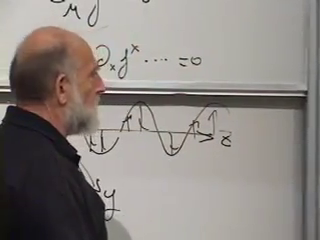
\includegraphics[width=0.70\textwidth]{lecture_58_figure_05.png}
\caption{Завершённый рисунок на доске поперечной электромагнитной волны: электрические и магнитные колебания перпендикулярны друг другу и направлению распространения.}
\lectureframe{01:05:25}
\end{figure}

\begin{figure}[H]
\centering
\scalebox{0.90}{%
\begin{tikzpicture}[x=1cm,y=1cm,>=Latex]
  \draw[->,thick] (0,0) -- (8.2,0) node[right] {$z$};
  \draw[->,thick] (0,-1.6) -- (0,1.7) node[above] {$x$};
  \draw[->,thick] (0,0) -- (-1.15,-0.8) node[below left] {$y$};
  \draw[blue!70!black,thick,domain=0:7.5,samples=120]
    plot (\x,{0.95*sin(90*\x)});
  \foreach \z/\s in {0.8/1,2.8/-1,4.8/1,6.8/-1}{
    \draw[->,green!45!black,thick]
      (\z,0) -- ++({-0.55*\s},{-0.38*\s});
  }
  \node[blue!70!black] at (6.9,1.25) {$\mathbf E$};
  \node[green!45!black] at (5.2,-1.05) {$\mathbf B$};
  \draw[->,very thick] (6.2,1.55) -- (7.7,1.55)
    node[midway,above] {propagation};
\end{tikzpicture}
}
\caption{Поля \(\mathbf E\) и \(\mathbf B\) перпендикулярны друг другу и направлению распространения.}
\end{figure}

Таков характер света и всего электромагнитного излучения в вакууме. Поскольку уравнения, из которых получена эта волна, лоренц-ковариантны, другой инерциальный наблюдатель тоже описывает электромагнитную волну, движущуюся со скоростью \(c\), с поперечными электрическим и магнитным полями.

\section{Плотность заряда и плотность тока}

Теперь мы возвращаем источники, которые были временно оставлены в стороне. Когда в некоторой области находится много заряженных частиц, полезно перейти к их грубозернистому описанию в виде непрерывной плотности заряда
\begin{equation}
\rho(\mathbf x,t)=\frac{dQ}{dV}.
\end{equation}
Это приближение похоже на рассмотрение воды как сплошной жидкости, хотя она состоит из молекул. Положительные и отрицательные заряды вносят вклады с противоположными знаками, так что \(\rho\) — это суммарный заряд на единицу объёма.

Заряд в выбранной области \(V\) равен
\begin{equation}
Q_V(t)=\int_V\rho(\mathbf x,t)\,dV.
\label{eq:charge-volume}
\end{equation}
Плотность может зависеть от положения и времени. Скопление заряда может уйти от точки, изменив там локальную плотность. Однако она не может изменяться произвольным образом. В природе электрический заряд сохраняется.

Одного лишь глобального закона сохранения было бы недостаточно. Он допускал бы, что заряд исчезает с Земли и в то же мгновение появляется на Марсе, тогда как полный заряд остаётся неизменным. Более сильное утверждение является локальным: заряд может покинуть одно место и попасть в другое только посредством потока через промежуточное пространство.

Чтобы описать этот поток, рассмотрим бесконечно малый ориентированный элемент поверхности
\begin{equation}
d\boldsymbol\sigma=\widehat{\mathbf n}\,d\sigma.
\end{equation}
Его модуль равен площади, а его направление перпендикулярно поверхности. Плотность тока \(\mathbf J\) определяется так, что заряд, пересекающий этот элемент в единицу времени, равен
\begin{equation}
\frac{dQ}{dt}=\mathbf J\cdot d\boldsymbol\sigma.
\label{eq:current-flux-element}
\end{equation}
Модуль \(\mathbf J\) имеет размерность заряда на единицу площади в единицу времени, а его направление совпадает с направлением потока положительного заряда.

\begin{figure}[H]
\centering
\includegraphics[width=0.64\textwidth]{lecture_58_figure_10.png}
\caption{Ориентированный элемент площади и множитель потока \(d\boldsymbol\sigma\cdot\mathbf J\).}
\lectureframe{01:18:15}
\end{figure}

Скалярное произведение выделяет компоненту, нормальную к поверхности. Ток, касательный к поверхности, не пересекает её и даёт нулевой вклад. Ток, параллельный нормали, даёт максимальный поток при фиксированном модуле. Ток в проводе — один частный случай, но \(\mathbf J\) может также описывать заряд, текущий через лист или через всё трёхмерное пространство.

\section{Локальное сохранение и уравнение непрерывности}

Зафиксируем область \(V\) в пространстве и направим наружу каждый элемент её замкнутой границы \(\partial V\). Если имеется суммарный направленный наружу ток, заряд внутри уменьшается:
\begin{equation}
\frac{dQ_V}{dt}
=-\oint_{\partial V}\mathbf J\cdot d\boldsymbol\sigma.
\label{eq:integral-conservation}
\end{equation}
Знак минус имеет физическую, а не условную природу: положительный поток наружу уносит положительный заряд из области. Используя уравнение~\eqref{eq:charge-volume},
\begin{equation}
\int_V\partial_t\rho\,dV
=-\oint_{\partial V}\mathbf J\cdot d\boldsymbol\sigma.
\label{eq:integral-continuity-one}
\end{equation}

\begin{figure}[H]
\centering
\includegraphics[width=0.72\textwidth]{lecture_58_figure_11.png}
\caption{Закон сохранения для фиксированной области после преобразования поверхностного потока в объёмное соотношение.}
\lectureframe{01:29:00}
\end{figure}

Теорема Гаусса, также называемая теоремой о дивергенции, связывает поток через замкнутую поверхность с дивергенцией внутри неё:
\begin{equation}
\oint_{\partial V}\mathbf A\cdot d\boldsymbol\sigma
=\int_V\boldsymbol\nabla\cdot\mathbf A\,dV.
\label{eq:divergence-theorem}
\end{equation}
Можно представить себе скрытые трубы, подающие воду в точки внутри сосуда. Дивергенция измеряет локальную скорость, с которой вода выходит из концов труб; поверхностный интеграл измеряет полное количество воды, покидающей сосуд. Всё, что создаётся внутри как направленный наружу поток, в конце концов должно пересечь границу.

Применяя уравнение~\eqref{eq:divergence-theorem} к \(\mathbf J\), получаем
\begin{equation}
\int_V
\left(\partial_t\rho+\boldsymbol\nabla\cdot\mathbf J\right)dV=0.
\end{equation}
Это соотношение верно для любой области \(V\). Следовательно, подынтегральное выражение должно обращаться в нуль в каждой точке:
\begin{equation}
\boxed{\partial_t\rho+\boldsymbol\nabla\cdot\mathbf J=0.}
\label{eq:continuity-three}
\end{equation}

\begin{figure}[H]
\centering
\includegraphics[width=0.72\textwidth]{lecture_58_figure_12.png}
\caption{Локальное уравнение непрерывности, записанное покомпонентно.}
\lectureframe{01:29:50}
\end{figure}

Уравнение~\eqref{eq:continuity-three} выражает в точности то, чего требует локальное сохранение. Если плотность заряда уменьшается в точке или внутри малой области, ток должен расходиться наружу из неё. Если ток сходится внутрь, плотность заряда увеличивается.

Плотность заряда и плотность тока естественно образуют четырёхток
\begin{equation}
J^\mu=(\rho,J_x,J_y,J_z)
\label{eq:four-current}
\end{equation}
в единицах \(c=1\). Уравнение непрерывности принимает вид лоренц-скалярного уравнения
\begin{equation}
\partial_\mu J^\mu=0.
\label{eq:continuity-four}
\end{equation}
Поток релятивистского распределения должен преобразовываться как четырёхвектор, так же как четырёхскорость отдельной частицы. Уравнение~\eqref{eq:continuity-four} делает локальное сохранение заряда справедливым во всех инерциальных системах отсчёта.

\section{Уравнения Максвелла с источниками}

При восстановлении заряда и тока получаем
\begin{align}
\boldsymbol\nabla\cdot\mathbf E&=\rho,
\label{eq:gauss-e-source}\\
\boldsymbol\nabla\cdot\mathbf B&=0,\\
\boldsymbol\nabla\times\mathbf E&=-\partial_t\mathbf B,\\
\boldsymbol\nabla\times\mathbf B&=\partial_t\mathbf E+\mathbf J.
\label{eq:ampere-source}
\end{align}
Уравнения с электрическими источниками сводятся к
\begin{equation}
\boxed{\partial_\mu F^{\mu\nu}=J^\nu,}
\label{eq:maxwell-source-covariant}
\end{equation}
тогда как магнитная пара без источников сохраняет вид
\begin{equation}
\boxed{\partial_\mu\widetilde F^{\mu\nu}=0.}
\label{eq:maxwell-dual-source}
\end{equation}

\begin{figure}[H]
\centering
\includegraphics[width=0.78\textwidth]{lecture_58_figure_13.png}
\caption{Уравнения Максвелла с источниками рядом с их ковариантной формой \(\partial_\mu F^{\mu\nu}=J^\nu\).}
\lectureframe{01:34:00}
\end{figure}

Временная компонента уравнения~\eqref{eq:maxwell-source-covariant} имеет вид
\begin{equation}
\partial_\mu F^{\mu t}=J^t=\rho,
\end{equation}
а уже выполненное покомпонентное вычисление превращает его левую часть в
\(\boldsymbol\nabla\cdot\mathbf E\). Три пространственные компоненты воспроизводят
\(\boldsymbol\nabla\times\mathbf B=\partial_t\mathbf E+\mathbf J\).

Есть и полезная проверка на согласованность. Применяя \(\partial_\nu\) к
уравнению~\eqref{eq:maxwell-source-covariant}, получаем
\begin{equation}
\partial_\nu J^\nu
=\partial_\nu\partial_\mu F^{\mu\nu}=0,
\end{equation}
поскольку две производные симметричны при \(\mu\leftrightarrow\nu\), тогда как \(F^{\mu\nu}\) антисимметричен.\editorialnote{Эта краткая проверка на согласованность следует из ковариантного уравнения и явно показывает, почему уравнения Максвелла с источниками автоматически удовлетворяют уравнению непрерывности.}

Теперь взаимная структура завершена. Тензорный закон силы
\(f^\mu=qF^\mu{}_\nu u^\nu\) описывает, как поля действуют на заряд, а
уравнение~\eqref{eq:maxwell-source-covariant} описывает, как заряд и ток порождают поля. Оба являются тензорными уравнениями. В вакууме те же уравнения поля дают поперечные волны, распространяющиеся со скоростью \(c\). Поэтому ковариантность Лоренца и уравнение электромагнитной волны сходятся в той точке, которая и мотивировала это построение: каждый инерциальный наблюдатель получает одни и те же законы электромагнетизма и одну и ту же скорость света.

\chapter{Собственное время, замедление времени и сокращение длины}

Мы часто будем выбирать единицы, в которых скорость света равна $c=1$. В этих единицах год времени и световой год расстояния можно сравнивать непосредственно, и формулы читать гораздо легче. Всякий раз, когда $c$ физически существенна, мы будем возвращать её обратно. Размерностного анализа достаточно, чтобы определить, где она должна стоять.

\section{Галилеева пространственно-временная сетка}

Начнем с доэйнштейновского соотношения между покоящейся системой отсчета и поездом, движущимся со скоростью $v$ вдоль оси $x$:
\begin{align}
x' &= x-vt, & t'&=t.
\label{eq:l4-galilean}
\end{align}
Во втором уравнении содержится ньютоновское предположение об универсальном времени. Все наблюдатели пользуются одними и теми же срезами одновременности, хотя пространственные начала координат движутся друг относительно друга.

Предположим, что нештрихованный наблюдатель стоит у пути, а штрихованный наблюдатель едет в поезде. Начало координат поезда имеет $x'=0$, поэтому его мировая линия в нештрихованных координатах имеет вид
\begin{equation}
x=vt.
\end{equation}
Эта наклонная прямая есть ось $t'$. Напротив, $t'=t$ означает, что все линии постоянного $t'$ — это те же горизонтальные линии, что и линии постоянного $t$.

\begin{figure}[H]
\centering
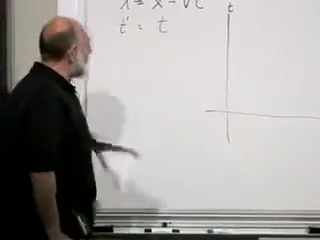
\includegraphics[width=0.72\textwidth]{lecture_04_figure_02.png}
\caption{Галилеево преобразование и исходная сетка $t$-$x$. Движущееся начало координат будет описывать $x=vt$, тогда как обе системы сохраняют общие линии постоянного времени.}
\lectureframe{00:03:06}
\end{figure}

Решая уравнение~\eqref{eq:l4-galilean} относительно нештрихованных координат, получаем
\begin{align}
x&=x'+vt'=x'+vt, & t&=t'.
\end{align}
Обратное преобразование имеет тот же вид, если заменить $v$ на $-v$. Если поезд движется вперед относительно станции, то станция движется назад относительно поезда. Эта взаимность сохраняется и в специальной теории относительности, а вот универсальное время — нет.

\section{Лоренцевская поправка}

Галилеевы преобразования не могут сделать скорость света одинаковой во всех инерциальных системах отсчета. Исправленные соотношения имеют вид, сначала в единицах $c=1$,
\begin{align}
x'&=\frac{x-vt}{\sqrt{1-v^2}}, &
t'&=\frac{t-vx}{\sqrt{1-v^2}}.
\label{eq:l4-lorentz-natural}
\end{align}
После восстановления обычных единиц получаем
\begin{align}
x'&=\frac{x-vt}{\sqrt{1-v^2/c^2}}, &
t'&=\frac{t-vx/c^2}{\sqrt{1-v^2/c^2}}.
\label{eq:l4-lorentz-c}
\end{align}

\begin{figure}[H]
\centering
\includegraphics[width=0.74\textwidth]{lecture_04_figure_05.png}
\caption{Преобразование Лоренца с восстановленными множителями $c$.}
\lectureframe{00:09:10}
\end{figure}

При $v\ll c$ и $v^2/c^2$, и $vx/c^2$ малы в тех условиях, где используется ньютоновская механика. Тогда уравнение~\eqref{eq:l4-lorentz-c} сводится к галилеевскому результату. Теория относительности не отбрасывает ньютоновскую кинематику; она устанавливает область её применимости.

При $v=c$ знаменатель обращается в нуль. Одна инерциальная система отсчета не может двигаться со скоростью света относительно другой инерциальной системы отсчета. Значительно ниже этого предела поправки малы, но вблизи него смешивание $x$ и $t$ становится неизбежным.

Движение выбрано вдоль $x$, поэтому поперечные координаты не меняются:
\begin{equation}
y'=y,\qquad z'=z.
\end{equation}
Один из способов понять, почему, — разместить одинаковые поперечные метровые стержни в поезде и на платформе. Наблюдатель в системе отсчета, промежуточной между двумя данными системами, видит, что стержни сближаются с равными по модулю и противоположными по направлению скоростями. В этой постановке нет ничего, что могло бы сделать один поперечный стержень короче другого.

\section{Преобразования Лоренца вдоль светового конуса}

Уравнение~\eqref{eq:l4-lorentz-natural} можно истолковать геометрически. Сложим два его уравнения:
\begin{align}
t'+x'
&=\frac{(t-vx)+(x-vt)}{\sqrt{1-v^2}}\\
&=(t+x)\frac{1-v}{\sqrt{1-v^2}}\\
&=(t+x)\sqrt{\frac{1-v}{1+v}}.
\label{eq:l4-null-plus}
\end{align}
Вычтем их в обратном порядке:
\begin{align}
t'-x'
&=\frac{(t-vx)-(x-vt)}{\sqrt{1-v^2}}\\
&=(t-x)\frac{1+v}{\sqrt{1-v^2}}\\
&=(t-x)\sqrt{\frac{1+v}{1-v}}.
\label{eq:l4-null-minus}
\end{align}

\begin{figure}[H]
\centering
\includegraphics[width=0.75\textwidth]{lecture_04_figure_06.png}
\caption{Преобразование Лоренца, переписанное через нулевые комбинации
$t+x$ и $t-x$. Их коэффициенты масштабирования взаимно обратны.}
\lectureframe{00:18:45}
\end{figure}

Комбинации $t+x$ и $t-x$ являются координатами вдоль двух светоподобных направлений под $45^\circ$. Буст сжимает одно из этих направлений и растягивает другое с обратным коэффициентом. Он не отклоняет ни одно из них от $45^\circ$. Поэтому световые лучи остаются световыми лучами; такова пространственно-временная картина инвариантности скорости света.

\begin{classroomqa}
\audiencequestion{Наблюдатель промежуточной системы видит симметричный эксперимент, но как из этого следует результат для наблюдателей в поезде и на платформе?\lecturetimestamp{00:20:48}}
\lecturerresponse{Используется еще один факт: совпадение событий инвариантно. Если концы стержней встречаются, то эта встреча представляет собой одно пространственно-временное событие. Любой инерциальный наблюдатель может приписать ему разные координаты, но ни один не может расщепить одно совпадение на два разных места. Вспышки, испускаемые там, где встречаются соответствующие концы, делают эти события операционально обнаружимыми. Симметрия промежуточной системы и инвариантность двух совпадений на концах устанавливают, что поперечные длины одинаковы.}
\end{classroomqa}

\begin{classroomqa}
\audiencequestion{Должен ли велосипедист, представляющий промежуточную систему отсчета, физически находиться в середине между стержнями?\lecturetimestamp{00:22:25}}
\lecturerresponse{Нет. Система отсчета — это целая сеть наблюдателей и часов, а не один глаз в одной точке. Велосипедист может получить вспышки от концов позже и заключить, где они были испущены. Существенно пространственно-временное положение каждого события излучения, а не то, где свет в конечном счете принимается.}
\end{classroomqa}

Сложение скоростей — еще одно следствие того же преобразования, но оно намеренно оставлено до следующей лекции. Наша нынешняя задача — выделить инвариантную величину, которую измеряют движущиеся часы.

\section{Инвариантный интервал}

При повороте обычных декартовых осей величина $x^2+y^2$ не изменяется. Преобразования Лоренца сохраняют другую квадратичную форму. Из уравнения~\eqref{eq:l4-lorentz-natural} получаем
\begin{align}
t'^2-x'^2
&=\frac{(t-vx)^2-(x-vt)^2}{1-v^2}\\
&=\frac{t^2-2vtx+v^2x^2-x^2+2vtx-v^2t^2}{1-v^2}\\
&=t^2-x^2.
\label{eq:l4-interval}
\end{align}
Смешанные члены сокращаются, а в оставшемся числителе содержится общий множитель $1-v^2$.

\begin{figure}[H]
\centering
\includegraphics[width=0.76\textwidth]{lecture_04_figure_07.png}
\caption{Вывод на доске равенства $t'^2-x'^2=t^2-x^2$.}
\lectureframe{00:33:15}
\end{figure}

В трех пространственных измерениях инвариант имеет вид
\begin{equation}
t'^2-x'^2-y'^2-z'^2=t^2-x^2-y^2-z^2
\end{equation}
в единицах $c=1$. В более общем случае для двух событий используются разности координат:
\begin{equation}
\Delta s^2
=c^2\Delta t^2-\Delta x^2-\Delta y^2-\Delta z^2.
\label{eq:l4-spacetime-interval}
\end{equation}
Все инерциальные наблюдатели согласны относительно этого числа, хотя относительно его отдельных временной и пространственных составляющих они не согласны.

\section{Собственное время и движущиеся часы}

Представьте себе решетку покоящихся наблюдателей, часы которых синхронизированы путем обмена световыми сигналами. Их показания определяют координатное время $t$. Теперь пронесем одни ручные часы через эту решетку. Их собственное показание сопровождает их вдоль мировой линии; это показание и есть собственное время.

Для двух временеподобно разделенных событий определим
\begin{equation}
c^2\Delta\tau^2
=c^2\Delta t^2-\Delta x^2-\Delta y^2-\Delta z^2.
\label{eq:l4-proper-time}
\end{equation}
В одном пространственном измерении при $c=1$ это просто
\begin{equation}
\Delta\tau=\sqrt{\Delta t^2-\Delta x^2}.
\end{equation}
Квадратный корень здесь аналогичен формуле для обычного расстояния, но знак минус меняет геометрию.

Имеются три случая:
\begin{align}
\Delta t^2-\Delta x^2 &>0 &&\text{timelike},\\
\Delta t^2-\Delta x^2 &=0 &&\text{lightlike},\\
\Delta t^2-\Delta x^2 &<0 &&\text{spacelike}.
\end{align}
Внутри светового конуса собственное время действительно. На самом конусе, где $x=\pm t$, оно равно нулю, хотя события не обязаны совпадать. Именно такие события может соединять световой луч. Вне конуса разделение пространственноподобно; его лучше описывать действительным собственным расстоянием $\sqrt{\Delta x^2-\Delta t^2}$, чем мнимым временем часов.

\begin{figure}[H]
\centering
\includegraphics[width=0.73\textwidth]{lecture_04_figure_08.png}

\vspace{0.8em}

\begin{tikzpicture}[x=1.0cm,y=1.0cm]
\draw[->] (-3.3,0) -- (3.3,0) node[right] {$x$};
\draw[->] (0,-0.4) -- (0,4.0) node[above] {$t$};
\draw[thick] (0,0) -- (3.0,3.0) node[above right] {$x=t$};
\draw[thick] (0,0) -- (-3.0,3.0) node[above left] {$x=-t$};
\node at (0,2.0) {timelike};
\node at (2.25,1.05) {spacelike};
\node at (-2.25,1.05) {spacelike};
\end{tikzpicture}
\caption{Световой конус на доске и четкая классификация временеподобного,
светоподобного и пространственноподобного разделения.}
\lectureframe{00:38:40}
\end{figure}

Почему формула~\eqref{eq:l4-proper-time} дает показание часов? Для часов, находящихся в покое, $\Delta x=0$, так что $\Delta\tau=\Delta t$. Для равномерно движущихся часов выберем штрихованную систему, в которой эти часы покоятся. Там $\Delta x'=0$, и инвариантность дает
\begin{equation}
\Delta\tau
=\sqrt{\Delta t'^2-\Delta x'^2}
=\Delta t'.
\end{equation}
Следовательно, движущиеся часы отсчитывают собственное время.

\begin{classroomqa}
\audiencequestion{Используются ли ``интервал между событиями'' и ``показание часов'' как два названия одного и того же?\lecturetimestamp{00:44:49}}
\lecturerresponse{Они совпадают, когда идеальные часы движутся по инерции от одного события к другому. Инвариантный интервал — геометрическая величина; разность показаний сопутствующих часов в начальном и конечном событиях дает его физическое измерение. Стационарные координатные часы, как правило, регистрируют иной интервал координатного времени.}
\end{classroomqa}

\section{Замедление времени и одновременность}

Рассмотрим начало движущейся системы отсчета. Его мировая линия задается соотношениями
\begin{equation}
x'=0,\qquad x=vt.
\end{equation}
Та же наклонная прямая является и траекторией движущихся часов, и осью $t'$.

\begin{figure}[H]
\centering
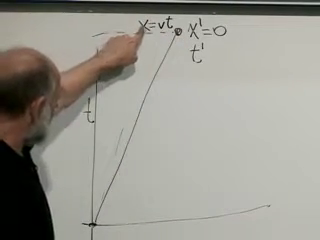
\includegraphics[width=0.72\textwidth]{lecture_04_figure_03.png}
\caption{Движущееся начало координат: $x=vt$, $x'=0$ и ось $t'$ — это три описания одной и той же мировой линии.}
\lectureframe{00:48:18}
\end{figure}

Применим инвариантный интервал между общим началом координат и более поздней точкой на этой мировой линии:
\begin{align}
t'^2-x'^2&=t^2-x^2,\\
t'^2&=t^2-v^2t^2,\\
t'&=t\sqrt{1-v^2}.
\label{eq:l4-time-dilation-natural}
\end{align}
После восстановления $c$ получаем
\begin{equation}
\Delta\tau=\Delta t\sqrt{1-\frac{v^2}{c^2}}
=\frac{\Delta t}{\gamma},
\qquad
\gamma=\frac{1}{\sqrt{1-v^2/c^2}}.
\label{eq:l4-time-dilation}
\end{equation}

\begin{figure}[H]
\centering
\includegraphics[width=0.73\textwidth]{lecture_04_figure_09.png}
\caption{Результат для замедления времени на доске: движущиеся часы отсчитывают
$t'=t\sqrt{1-v^2}$ в единицах, где $c=1$.}
\lectureframe{00:50:45}
\end{figure}

Неподвижный наблюдатель говорит, что движущиеся часы идут медленнее. Принцип взаимности требует, чтобы движущийся наблюдатель говорил то же самое о неподвижных часах. Противоречия нет, потому что эти два описания сравнивают разные пары удалённых событий.

Действительно, постоянное значение $t'$ в уравнении~\eqref{eq:l4-lorentz-natural} удовлетворяет
\begin{equation}
t-vx=\text{constant}.
\label{eq:l4-simultaneity}
\end{equation}
Линии одновременности движущегося наблюдателя наклонены относительно горизонтальных линий $t=\text{constant}$. Каждый наблюдатель считает одновременным свой набор показаний удалённых часов. Если ясно удерживать это различие, взаимное замедление часов оказывается непротиворечивым.

\begin{figure}[H]
\centering
\begin{tikzpicture}[x=1cm,y=1cm]
\draw[->] (0,0) -- (0,4.2) node[above] {$t$};
\draw[->] (0,0) -- (5.2,0) node[right] {$x$};
\draw[thick,->] (0,0) -- (2.4,3.8) node[above] {$x'=0$};
\draw[dashed] (0,2.8) -- (4.8,2.8)
  node[right] {$t=\mathrm{const}$};
\draw[thick] (0.15,1.05) -- (4.7,2.35)
  node[right] {$t'=\mathrm{const}$};
\draw[thick] (3.4,0) -- (3.4,3.8);
\fill (3.4,2.8) circle (0.045);
\fill (3.4,1.98) circle (0.045);
\end{tikzpicture}
\caption{При взаимном замедлении времени сравниваются показания часов на разных срезах одновременности.}
\end{figure}

\section{Пути близнецов}

Два близнеца начинают в одном и том же событии. Один остаётся при $x=0$. Другой удаляется со скоростью $v$, меняет направление и возвращается с той же скоростью. Когда они снова встречаются, они сравнивают все физические процессы, которые могут служить часами: наручные часы, сердцебиение, обмен веществ или само старение.

Пусть каждая половина путешествия занимает координатное время $T$ в домашней системе отсчёта. Собственное время домашнего близнеца равно
\begin{equation}
\tau_{\mathrm{home}}=2T.
\end{equation}
Событие разворота имеет координаты $(vT,T)$. Поэтому первый участок пути путешествующего близнеца даёт вклад
\begin{align}
\tau_{\mathrm{leg}}
&=\sqrt{T^2-v^2T^2}
=T\sqrt{1-v^2}.
\end{align}
Обратный участок даёт такую же величину, следовательно,
\begin{equation}
\tau_{\mathrm{travel}}=2T\sqrt{1-v^2}<2T.
\label{eq:l4-twin}
\end{equation}

\begin{figure}[H]
\centering
\includegraphics[width=0.73\textwidth]{lecture_04_figure_10.png}

\vspace{0.8em}

\begin{tikzpicture}[x=1.1cm,y=1cm]
\draw[->] (-0.2,0) -- (3.4,0) node[right] {$x$};
\draw[->] (0,-0.1) -- (0,4.4) node[above] {$t$};
\draw[very thick] (0,0) -- (0,4);
\draw[very thick] (0,0) -- (2.2,2) -- (0,4);
\draw[dashed] (0,2) -- (2.2,2);
\node[left] at (0,2) {$T$};
\node[left] at (0,4) {$2T$};
\node[below right] at (1.1,1.0) {$v$};
\node[above right] at (1.1,3.0) {$-v$};
\end{tikzpicture}
\caption{Мировая линия домашнего близнеца и два участка пути путешествующего. Их собственные времена различны, потому что это разные пути в пространстве-времени.}
\lectureframe{00:59:35}
\end{figure}

В неравенстве возрастов нет противоречия. Траектория путешественника содержит поворот и не связана с прямой домашней траекторией единым преобразованием симметрии между инерциальными системами отсчёта. В обычной евклидовой геометрии прямой маршрут и ломаный маршрут между двумя точками тоже имеют разные длины. Геометрия Минковского меняет местами то, у какого пути интервал больше, но само сравнение остаётся геометрическим.

\section{Ускорение и идеальные часы}

\begin{classroomqa}
\audiencequestion{При развороте физика иная, и путешественник ускоряется. Не делает ли это расчёт по показаниям часов недействительным?
\lecturetimestamp{01:02:19}}
\lecturerresponse{Ускорение реально и помогает выявить асимметрию; не следует от него отмахиваться. Острый угол — лишь идеализированный рисунок, и его можно сгладить, заменив разворотом конечной длительности. Дополнительное физическое предположение состоит в том, что достаточно малые и хорошо устроенные часы нечувствительны к умеренному ускорению и продолжают отсчитывать собственное время. Большие или хрупкие часы могут деформироваться или сломаться, но это недостаток механизма, а не пространственно-временного интервала.}
\end{classroomqa}

Это предположение об идеальных часах не выводится из одного лишь преобразования Лоренца. Его проверяют по поведению реальных часовых механизмов. Атом является гораздо лучшим приближением, чем часы размером в сотни миль, потому что компактный механизм труднее деформировать под действием ускорения или гравитации. Простое упоминание общей теории относительности не устранило бы этой физической проблемы; всё равно пришлось бы знать, как выбранный механизм реагирует на окружающие условия.

\begin{classroomqa}
\audiencequestion{Можно ли свести ускоренную траекторию к коротким интервалам, на которых инерциальный анализ остаётся применимым?\lecturetimestamp{01:09:08}}
\lecturerresponse{Да. Разбейте кривую на короткие, почти прямые отрезки, вычислите собственное время на каждом отрезке и сложите результаты. Это пространственно-временной аналог нахождения длины обычной кривой из многих малых отрезков. В пределе непрерывности,
\[
\tau=\int \sqrt{1-\frac{v(t)^2}{c^2}}\,dt,
\]
для движения в плоском пространстве-времени, описанного в инерциальной системе координат.}
\end{classroomqa}

\section{Что видят близнецы}

Окончательные показания часов можно операционально задать, посылая световые импульсы. Отметьте на обеих мировых линиях интервалы собственного времени по одной секунде и пусть каждый близнец испускает импульс на каждой отметке. На участке удаления импульсы, получаемые от другого близнеца, приходят с большими промежутками. На участке возвращения они приходят плотной группой. Это релятивистский эффект Доплера, непосредственно выраженный на пространственно-временной диаграмме.

\begin{figure}[H]
\centering
\includegraphics[width=0.73\textwidth]{lecture_04_figure_11.png}
\caption{Световые сигналы между домашней мировой линией и мировой линией путешественника. Редкие приходы на участке удаления и сближенные на участке возвращения позволяют учесть каждый испущенный импульс.}
\lectureframe{01:12:55}
\end{figure}

Ни одна система отсчёта в этом рассказе не исчезает. Каждый наблюдатель в конце концов получает все импульсы, испущенные другим, но частота их приёма зависит от относительного движения. Красное смещение на удалении и синее смещение на сближении действуют для двух путей не в течение одинаковых промежутков времени, поэтому подсчёт всех принятых импульсов согласуется со сравнением собственных времён.

\begin{classroomqa}
\audiencequestion{Если возвращающийся путешественник принимает свет, смещённый в синюю сторону, может ли он собрать больше энергии, чем излучил источник?
\lecturetimestamp{01:13:50}}
\lecturerresponse{Для этого вопроса нужны релятивистское определение энергии и её зависимость от системы отсчёта, которые мы ещё не ввели. Это разумный вопрос, но одних лишь координат и подсчёта импульсов недостаточно, чтобы свести энергетический баланс, особенно для ускоренного наблюдателя. Поэтому ответ лучше отложить, а не угадывать.}
\end{classroomqa}

\section{Замкнутое пространственное направление}

\begin{classroomqa}
\audiencequestion{Предположим, что одно пространственное направление компактно. Может ли близнец равномерно двигаться вдоль него, вернуться в исходную точку и вовсе обойтись без ускорения? Что тогда различает близнецов?\lecturetimestamp{01:15:14}}
\lecturerresponse{Пространство следует представлять внутренне как цилиндр, а не как лист, изогнутый внутри большего пространства; радиального ускорения может вовсе не быть. Тем не менее возвращающийся наблюдатель сталкивается с глобальным фактом: одни и те же места повторяются. Это указывает на асимметрию, но полный ответ требует аккуратного рассмотрения специальной теории относительности при таком пространственном отождествлении. Здесь вопрос оставлен открытым, а не закрыт импровизированным ответом.}
\end{classroomqa}

\begin{figure}[H]
\centering
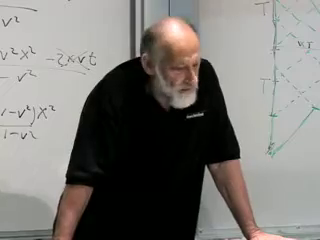
\includegraphics[width=0.72\textwidth]{lecture_04_figure_04.png}

\vspace{0.8em}

\begin{tikzpicture}[x=1cm,y=1cm]
\draw[thick] (0,0) ellipse (1.3 and 0.35);
\draw[thick] (-1.3,0) -- (-1.3,-3.1);
\draw[thick] (1.3,0) -- (1.3,-3.1);
\draw[thick] (0,-3.1) ellipse (1.3 and 0.35);
\draw[->,very thick] (0.0,0.38) arc (90:-210:1.38 and 0.42);
\node[right] at (1.65,-1.5) {compact spatial direction};
\end{tikzpicture}
\caption{Вопрос о компактном пространстве в том виде, как он нарисован на доске, с чисто внутренне заданным цилиндром. Это вопрос о глобальном отождествлении, а не о движении вокруг цилиндра, вложенного в дополнительное радиальное измерение.}
\lectureframe{01:17:56}
\end{figure}

\section{Длина измеряется на срезе одновременности}

В задаче по специальной теории относительности сначала нарисуйте пространственно-временную картину. Возьмите метровый стержень, покоящийся в нештрихованной системе отсчёта, с концами при $x=0$ и $x=1$. С течением времени оба конца прочерчивают вертикальные мировые линии. Стержень заметает между ними ленту.

Движущийся наблюдатель должен измерить оба конца при одном значении движущегося времени $t'$. Из уравнения~\eqref{eq:l4-simultaneity} следует, что срез, проходящий через начало координат и имеющий $t'=0$, удовлетворяет
\begin{equation}
t=vx
\end{equation}
в единицах $c=1$. Он пересекает правый конец $x=1$ при $t=v$.

\begin{figure}[H]
\centering
\includegraphics[width=0.73\textwidth]{lecture_04_figure_12.png}

\vspace{0.8em}

\begin{tikzpicture}[x=1.55cm,y=1.15cm]
\draw[->] (-0.5,0) -- (3.1,0) node[right] {$x$};
\draw[->] (0,0) -- (0,3.8) node[above] {$t$};
\draw[very thick,red] (0,0) -- (0,3.3);
\draw[very thick,red] (2.15,0) -- (2.15,3.3);
\fill[red!12] (0,0) rectangle (2.15,3.3);
\draw[very thick,green!50!black] (0,0) -- (1.2,3.1)
  node[above] {$x=vt$};
\draw[very thick,blue] (0,0) -- (2.15,1.15)
  node[right] {$t'=0$};
\fill (2.15,1.15) circle (0.045);
\node[right] at (2.22,1.35) {$(x,t)=(1,v)$};
\node[below] at (2.15,0) {$1$};
\end{tikzpicture}
\caption{Покоящийся стержень заметает пространственно-временную ленту. Длина, измеряемая движущимся наблюдателем, есть расстояние между его концами на одном срезе $t'=\mathrm{const}$.}
\lectureframe{01:24:20}
\end{figure}

Выбранное разделение концов пространственноподобно, поэтому используем положительную пространственную форму инварианта:
\begin{equation}
x'^2-t'^2=x^2-t^2.
\end{equation}
В выбранном конце $t'=0$, $x=1$ и $t=v$. Следовательно,
\begin{align}
x'^2&=1-v^2,\\
x'&=\sqrt{1-v^2}.
\end{align}
Таким образом, собственная длина $L$ измеряется в движущейся системе как
\begin{equation}
L'=L\sqrt{1-v^2/c^2}=\frac{L}{\gamma}.
\label{eq:l4-length-contraction}
\end{equation}

\begin{figure}[H]
\centering
\includegraphics[width=0.76\textwidth]{lecture_04_figure_13.png}
\caption{Завершённое построение сокращения длины и полученный на доске результат $x'=\sqrt{1-v^2}$ для единичной собственной длины.}
\lectureframe{01:28:10}
\end{figure}

Верно и обратное утверждение: наблюдатель на платформе приписывает меньшую длину продольному метровому стержню в поезде. И снова два наблюдателя выбирают разные одновременные события на концах, поэтому взаимность здесь не ведёт к противоречию.

\section{Вопросы в конце}

\begin{classroomqa}
\audiencequestion{Распространяется ли что-нибудь, кроме света, со скоростью света? В частности, как обстоит дело с гравитацией?\lecturetimestamp{01:29:29}}
\lecturerresponse{Общая теория относительности предсказывает гравитационные волны, распространяющиеся со скоростью $c$. Во время этой лекции свидетельства были косвенными и исходили от таких систем, как двойные пульсары; гравитационные волны ещё не были непосредственно обнаружены.\editorialnote{После этой лекции 2006 года экспериментальная ситуация изменилась. LIGO непосредственно зарегистрировал GW150914 в 2015 году, а совместное наблюдение GW170817 и его электромагнитного аналога в 2017 году показало, что скорости распространения гравитации и света совпадают с точностью до нескольких частей на $10^{15}$. См. \url{https://ligo.org/detections/gw150914/} и \url{https://doi.org/10.1103/PhysRevLett.119.251302}.}}
\end{classroomqa}

\begin{classroomqa}
\audiencequestion{Может ли астронавт преодолеть расстояние во много световых лет за собственное время, меньшее, чем это расстояние, выраженное в световых годах? Означало бы это движение быстрее света?\lecturetimestamp{01:30:38}}
\lecturerresponse{Собственное время астронавта равно $\sqrt{\Delta t^2-\Delta x^2}$, что меньше координатного времени $\Delta t$. В инерциальной системе астронавта расстояние между звёздами сокращено по Лоренцу. Звёзды движутся со скоростью $-v$, а не быстрее света; просто нужно пересечь меньшее, сокращённое расстояние.}
\end{classroomqa}

Если астронавт начинает из состояния покоя и разгоняется, описание меняется при переходе от одной мгновенно сопутствующей инерциальной системы отсчёта к другой. При этом расстояние, приписываемое звёздам, может меняться. Нельзя применить одно фиксированное преобразование Лоренца ко всей истории с ускорением, но полное собственное время всё равно получается суммированием вкладов вдоль мировой линии. То же самое относится и к реалистичному близнецу, который стартует, разворачивается и тормозит, а не рождается уже на крейсерской скорости.

\begin{classroomqa}
\audiencequestion{Вызваны ли эти парадоксы тем, что мы считаем время чем-то особым? Должны ли мы называть его четвёртым измерением?\lecturetimestamp{01:36:43}}
\lecturerresponse{Необязательно начинать с лозунга о том, что время — четвёртое измерение. Само преобразование Лоренца приводит к смешению пространства и времени, а интервал $t^2-x^2-y^2-z^2$ рассматривает их как части единой геометрии, в которой у времени и пространства разные знаки. При малых скоростях это смешение становится пренебрежимо малым, и возвращается привычная ньютоновская интуиция. Однако при релятивистских скоростях пространство и время нельзя считать принципиально независимыми друг от друга.}
\end{classroomqa}

Поэтому замедление времени, сокращение длины, сравнение близнецов и сокращённое время в пути не являются отдельными уловками. Всё это вытекает из трёх привычек: определять сравниваемые события, изображать их геометрию в пространстве-времени и использовать инвариантный интервал.
\chapter{Огненные шары, системы отсчёта и четырёхвекторы}

Начнём с вопроса, оставшегося после обсуждения столкновений при высоких энергиях. Столкновение двух тяжёлых ядер создаёт бурно изменяющийся объект, а не спокойную астрофизическую чёрную дыру. Что же тогда может означать описание столкновения с помощью горизонта? Ответ проведёт нас через пятимерную картину сильносвязанной материи, ряд практических вопросов об ускорителях и, наконец, обратно к геометрии специальной теории относительности. К концу скорость и импульс станут четырёхвекторами, а энергия займёт место рядом с тремя компонентами импульса.

\section{Огненный шар в пятом измерении}

\begin{classroomqa}
\audiencequestion{Объект, возникающий при столкновении, неустойчив и меняет форму. Как такой сложный объект можно называть чёрной дырой?}
\lecturerresponse{Представьте себе пятое пространственное направление, идущее между полом и потолком. Гравитация в этом направлении тянет возбуждения к полу. Столкновение оставляет там горячий сгусток энергии; он растекается и меняет форму, но всё же может обладать горизонтом, температурой и энтропией.}
\end{classroomqa}

Представьте себе частицы или, если нагляднее, маленькие струны, движущиеся в этом пятимерном мире. Возбуждения, падающие к полу, в четырёх измерениях выглядят как адроны: протоны, нейтроны, мезоны и другие протяжённые составные объекты. Возбуждения, привязанные к области у потолка, выглядят более элементарными. Поэтому вертикальное положение служит геометрическим способом кодировать масштаб: пол соответствует адронному режиму больших расстояний, а потолок — степеням свободы на малых расстояниях.

Когда сталкиваются два адрона, два объекта у пола ударяются друг о друга и создают мощный всплеск энергии. Результат — не жёсткое тело. Это горячий сгусток с горизонтом, своего рода лужа в пятимерном гравитационном поле. Это не астрофизическая чёрная дыра в обычном четырёхмерном пространстве и не чёрная дыра планковского масштаба, прикреплённая к потолку. Это гравитационное описание сильно взаимодействующего огненного шара у пола.

При высокой энергии налетающие ядра из-за лоренцева сокращения превращаются в тонкие блины. Они сталкиваются, отдают свою энергию в малой области и порождают жидкость, которая растекается, приближаясь к равновесию. Её малая вязкость была одной из удивительных особенностей кварк--глюонной плазмы. В пятимерном описании та же эволюция представляет собой релаксацию искажённого горизонта.

\begin{figure}[H]
\centering
\includegraphics[width=0.82\textwidth]{lecture_05_figure_01.png}
\caption{Схема пятого измерения с полом и потолком. После столкновения центральный сгусток с горизонтом растекается вдоль пола.}
\lectureframe{00:04:22}
\end{figure}

Горизонт не сохраняется вечно. Излучение Хокинга уносит энергию, а в четырёхмерном описании это излучение есть каскад обычных адронов, выходящих из столкновения. Тысячи треков в событии детектора — это, на этом языке, частицы, выкипевшие из дуальной чёрной дыры.

\subsection{Реально ли дополнительное измерение?}

\begin{classroomqa}
\audiencequestion{Является ли пятое измерение пространственным, и действительно ли проведённая между полом и потолком линия буквально тянется в этом направлении?}
\lecturerresponse{Да. Оно пространственноподобно, а поверхность, изображённая в этой пятимерной геометрии, — это горизонт. Называть ли дополнительное направление ``реальным'' или рассматривать его как эквивалентное математическое описание — более глубокий вопрос.}
\end{classroomqa}

Полезное утверждение состоит не в том, что гравитация заменяет квантовую хромодинамику. Скорее, одну и ту же физику можно описывать двумя языками. В четырёхмерном языке есть горячий огненный шар из кварков и глюонов, без обычного гравитационного поля. В пятимерном языке есть гравитация и горизонт. Если соответствие верно, то полноценный расчёт в КХД и дуальный гравитационный расчёт должны совпадать всюду, где оба можно выполнить.

\begin{classroomqa}
\audiencequestion{В КХД нет ни гравитации, ни горизонтов. Добавляет ли картина с чёрной дырой новую физику или лишь по-новому описывает огненный шар?}
\lecturerresponse{В четырёх измерениях это плазма кварков и глюонов; в пятимерном воплощении у неё есть гравитационное описание с горизонтом. Преимущество здесь вычислительное. Сильносвязанная КХД чрезвычайно трудна, тогда как некоторые свойства горизонта---в частности вязкость---вычисляются сравнительно легко.}
\end{classroomqa}

Различие между ``реальным измерением'' и ``математической аналогией'' не нужно окончательно устанавливать, чтобы описание было полезным. Структура заслуживает физической интерпретации, когда она вместе с другими переменными образует более простой и более связный набор законов. Всё же не следует преувеличивать: применения калибровочно-гравитационной дуальности к наблюдаемой кварк--глюонной плазме являются моделями сильносвязанной динамики, а не доказательством того, что у реальной КХД есть известный точный гравитационный дуал.\editorialnote{Эта оговорка явно формулирует современный статус применения к КХД; она не меняет пятимерный механизм, развитый здесь.}

\section{Почему в коллайдерах сталкивают пучки}

Теперь вопросы становятся практическими. Почему используют два движущихся пучка вместо одного пучка и неподвижной мишени? Почему кольцевые ускорители так велики? Почему с электронами и протонами работают по-разному? Все эти вопросы — о релятивистской энергии.

\begin{classroomqa}
\audiencequestion{Почему сталкивают два пучка, а не направляют один энергичный пучок в неподвижную мишень?}
\lecturerresponse{Новые частицы создаёт энергия, доступная в системе центра масс. Два одинаковых и противоположно направленных релятивистских пучка не имеют суммарного импульса, поэтому для столкновения доступна практически вся их энергия. При неподвижной мишени значительная часть энергии налетающей частицы вынужденно остаётся в виде движения центра масс.}
\end{classroomqa}

Для двух ультрарелятивистских частиц с противоположными импульсами, модуль каждого из которых равен \(p\), оценка на уровне лекции в единицах \(c=1\) имеет вид
\begin{equation}
E_{\mathrm{cm}}^{\mathrm{collider}}\simeq 2p.
\end{equation}
Соответствующая оценка для неподвижной мишени растёт лишь как квадратный корень из импульса пучка,
\begin{equation}
E_{\mathrm{cm}}^{\mathrm{fixed}}\sim \sqrt{mp}.
\end{equation}
Здесь существен именно характер зависимости, а не опущенный численный множитель: удвоение энергии пучка удваивает энергию коллайдера, но для неподвижной мишени энергия центра масс при этом растёт лишь как квадратный корень.

Инвариантный расчёт делает это сравнение точным. Если \(P_1\) и \(P_2\) — входящие четырёхимпульсы, то
\begin{equation}
s=(P_1+P_2)^2,
\qquad E_{\mathrm{cm}}=\sqrt{s}.
\end{equation}
Для одинаковых встречных пучков с энергией \(E\) пространственные импульсы взаимно компенсируются, и \(\sqrt{s}=2E\). Для частицы с энергией \(E\gg m\), налетающей на покоящуюся мишень той же массы,
\begin{equation}
s=2m^2+2mE,
\qquad
\sqrt{s}\simeq \sqrt{2mE}
\qquad (c=1).
\end{equation}
Этот короткий инвариантный вывод даёт тот множитель, который был опущен в устной оценке.\editorialnote{Этот вывод включён, чтобы аргумент лекции о характере зависимости можно было воспроизвести.}

\begin{classroomqa}
\audiencequestion{Есть ли фундаментальная причина, по которой кольцевой ускоритель должен быть таким большим? Не мог бы тот же пучок просто больше раз проходить по машине меньшего размера?}
\lecturerresponse{Поля и материалы накладывают ограничения. Частица получает конечное приращение энергии на метр, поэтому установке большей энергии нужна большая эффективная длина ускорения. Малый радиус также требует большего поперечного ускорения, а ускоренный заряд излучает. Если кольцо слишком мало, пучок излучает энергию так же быстро, как машина её сообщает.}
\end{classroomqa}

Соотношение для изгиба траектории приближённо имеет вид
\begin{equation}
p=qBR,
\end{equation}
поэтому при фиксированном магнитном поле \(B\) больший импульс \(p\) требует большего радиуса \(R\). Работу по увеличению энергии пучка выполняют радиочастотные резонаторы; магниты изгибают и фокусируют пучок. Общий вывод остаётся тем же, что был сформулирован у доски: напряжённость поля и радиационные потери не позволяют сжать ускоритель сколь угодно высокой энергии в маленькое кольцо.

При движении по окружности ускорение есть даже при постоянной скорости, потому что меняется направление скорости. Ускоренный заряд испускает синхротронное излучение. Линейный ускоритель избегает непрерывных потерь на изгиб, хотя сами короткие ускоряющие толчки не являются в буквальном смысле свободными от излучения. Кольцевые машины принимают цену изгиба в обмен на повторное использование одной и той же аппаратуры на каждом обороте.

\begin{classroomqa}
\audiencequestion{Почему электроны связывали с линейным ускорителем в SLAC, тогда как в кольцевых высокоэнергетических коллайдерах используют протоны или другие адроны?}
\lecturerresponse{Электроны гораздо легче. При данной высокой энергии их фактор Лоренца намного больше, и круговое ускорение заставляет их излучать гораздо сильнее. Более тяжёлые протоны могут многократно обращаться по кольцу, набирая энергию на каждом проходе, прежде чем синхротронные потери станут недопустимо большими.}
\end{classroomqa}

При фиксированных энергии и радиусе кольца излучаемая мощность очень резко зависит от массы частицы,
\begin{equation}
P_{\mathrm{sync}}\propto \frac{E^4}{m^4R^2}.
\end{equation}
Вот почему различие электрон--протон гораздо резче, чем можно было бы подумать по фразе ``более лёгкая частица движется быстрее'': оба пучка уже могут двигаться чрезвычайно близко к \(c\), но их лоренц-факторы и потери на излучение очень различны.\editorialnote{Соотношение для изгиба и синхротронное масштабирование делают качественный аргумент лекции об ускорителях точным; на доске их не выводили.}

\begin{classroomqa}
\audiencequestion{Почему бы не ускорять адроны тоже по прямой?}
\lecturerresponse{Можно. Трудность — в длине установки. В кольце одна и та же частица много раз проходит через ускоряющие структуры; эквивалентный линейный адронный ускоритель должен был бы иметь огромную длину. Полезный компромисс — большое кольцо, достаточно большое, чтобы излучение протонов оставалось приемлемым.}
\end{classroomqa}

Эти вопросы об ускорителях ясно показывают, почему ньютоновских правил недостаточно. Теперь мы вернёмся к специальной теории относительности и введём язык, позволяющий проводить такие сравнения систематически.

\section{Гараж и лимузин}

Рассмотрим гараж длиной около двенадцати футов и длинный лимузин длиной около двадцати футов. Водитель разгоняется, пока лимузин не сократится по Лоренцу, надеясь, что тот поместится. В системе гаража движущийся лимузин короче, так что это кажется возможным. В системе лимузина, однако, короче движущийся гараж, так что это кажется невозможным. Может ли весь лимузин находиться внутри гаража?

Откроем обе двери, чтобы столкновение со стеной нас не отвлекало. Сказать, что лимузин находится внутри, значит, что его передняя и задняя части находятся внутри \emph{одновременно}. В этом последнем слове и заключена вся загадка.

Нарисуйте пространственно-временную диаграмму, где \(t\) отложено по вертикали, а \(x\) — по горизонтали. Лучи света образуют световой конус с углом \(45^\circ\) в единицах \(c=1\). Гараж покоится, поэтому мировые линии его двух дверей вертикальны. Передняя и задняя части лимузина задают две параллельные наклонные мировые линии. Ось \(t'\) движущейся системы наклонена к световому конусу, а её линии одновременности параллельны наклонённой оси \(x'\).

\begin{figure}[H]
\centering
\includegraphics[width=0.82\textwidth]{lecture_05_figure_02.png}
\caption{Готовая пространственно-временная диаграмма гараж--лимузин. Вертикальные линии ограничивают гараж; наклонные линии прослеживают два конца лимузина. Горизонтальные и наклонённые сечения представляют разные срезы одновременности в двух системах отсчёта.}
\lectureframe{00:31:05}
\end{figure}

В системе гаража горизонтальная линия может пересекать обе мировые линии лимузина между двумя мировыми линиями гаража. В этот момент по времени гаража задняя часть уже въехала, а передняя ещё не выехала. Сокращённый лимузин целиком находится внутри.

В системе лимузина соответствующие одновременные события лежат на наклонной линии. Проведите такую линию через событие, в котором задняя часть въезжает. Она пересечёт мировую линию передней части после того, как та уже прошла дальнюю дверь. Согласно собственной одновременности лимузина, он никогда не находится целиком внутри. Оба утверждения верны, потому что в них сравниваются разные пары событий.

\begin{classroomqa}
\audiencequestion{Образуют ли две зелёные мировые линии и горизонтальный отрезок между ними параллелограмм? Является ли этот чёрный отрезок длиной лимузина?}
\lecturerresponse{Горизонтальный отрезок — это лоренц-сокращённая длина, потому что его концы одновременны в системе гаража. Собственная длина определяется концами, одновременными в системе лимузина, на линии, параллельной \(x'\). В этих двух измерениях используются разные сечения одной и той же пары мировых линий.}
\end{classroomqa}

Если \(L_0\) — собственная длина, то горизонтальное сечение в системе гаража имеет длину
\begin{equation}
L=\frac{L_0}{\gamma},
\qquad
\gamma=\frac{1}{\sqrt{1-v^2/c^2}}.
\end{equation}
Сама формула парадокс не разрешает. Это делает диаграмма, потому что она показывает, какие события сравнивались. Всякий раз, когда задача по теории относительности как будто даёт два несовместимых ответа, ищите неявное употребление ``одновременно''.

\section{Четыре координаты и два положения индекса}

Чтобы перейти от парадоксов к законам движения, нам нужна запись, сохраняющая геометрию. Соберём координаты в виде
\begin{equation}
(X^1,X^2,X^3,X^0)=(x,y,z,t),
\qquad X^\mu=(x,y,z,t),
\end{equation}
где \(\mu\) принимает значения \(1,2,3,0\). Такой порядок помещает время в записи последним, хотя его индекс равен \(0\); это соответствует соглашению, использованному на доске.

\begin{classroomqa}
\audiencequestion{Мы полагаем \(c=1\)? Если вернуть обычные единицы, должна ли временная координата быть \(ct\)?}
\lecturerresponse{Да. Мы полагаем \(c=1\) при построении геометрии и возвращаем множители \(c\), когда важны размерности или нерелятивистский предел. При обычных единицах длины временная координата равна \(ct\).}
\end{classroomqa}

Один и тот же вектор можно записать и с нижним индексом. При используемом здесь соглашении о знаках,
\begin{equation}
X_\mu=(-x,-y,-z,t).
\end{equation}
Следовательно, опускание индекса меняет знаки трёх пространственных компонент и оставляет временную компоненту неизменной. Например,
\begin{equation}
X^\mu=(3,2,4,10)
\quad\Longrightarrow\quad
X_\mu=(-3,-2,-4,10).
\end{equation}
Это не две точки пространства-времени; это две компонентные формы одного геометрического объекта.

\begin{classroomqa}
\audiencequestion{Какие компоненты ковариантны, а какие контравариантны, и следует ли понимать эти обозначения как верхние или нижние индексы?}
\lecturerresponse{Компоненты с верхним индексом контравариантны; с нижним — ковариантны. Полезная мнемоника, прозвучавшая в аудитории: ``co — снизу, contra — сверху.'' Физики часто просто говорят «сверху» и «снизу».}
\end{classroomqa}

Эта запись оправдывает себя в инвариантной свёртке
\begin{equation}
X_\mu X^\mu=t^2-x^2-y^2-z^2.
\label{eq:l5-interval}
\end{equation}
В дифференциальной форме это имеет вид
\begin{equation}
d\tau^2=dt^2-dx^2-dy^2-dz^2
\qquad (c=1).
\label{eq:l5-proper-time}
\end{equation}
Для времениподобного движения \(d\tau\) — это время, показываемое часами, движущимися вдоль мировой линии.

Когда один и тот же индекс встречается один раз вверху и один раз внизу, подразумевается суммирование. Соглашение Эйнштейна превращает
\begin{equation}
\sum_{\mu}X_\mu X^\mu
\end{equation}
в более короткое выражение в уравнении~\eqref{eq:l5-interval}. Это не просто экономия записи. Оно избавляет от необходимости вручную переписывать чередующиеся знаки геометрии Минковского в каждом уравнении.

\begin{classroomqa}
\audiencequestion{Является ли \(\tau\) стандартным обозначением собственного времени?}
\lecturerresponse{Да. Символ \(s\) тоже иногда используется, но \(\tau\) — стандартный выбор для собственного времени.}
\end{classroomqa}

\section{Повороты как простая симметрия}

Лоренцев буст смешивает пространство и время. Прежде чем изучать эту матрицу, рассмотрим более привычную операцию поворота пространственных осей. Если относительное движение направлено произвольным образом, мы можем повернуть оси так, чтобы это направление стало новой осью \(x\), а затем применить известный буст. Поэтому повороты — часть построения, а не декоративное отступление.

Для поворота на угол \(\theta\) вокруг оси \(z\),
\begin{align}
x'&=x\cos\theta+y\sin\theta,\nonumber\\
y'&=-x\sin\theta+y\cos\theta,\label{eq:l5-rotation}\\
z'&=z.\nonumber
\end{align}
При \(\theta=0\) эти уравнения дают \(x'=x\) и \(y'=y\); при \(\theta=\pi/2\) они меняют оси местами с ожидаемыми знаками.

Это преобразование сохраняет евклидово расстояние. Обозначая \(c_\theta=\cos\theta\) и \(s_\theta=\sin\theta\),
\begin{align}
x'^2+y'^2
&=(xc_\theta+ys_\theta)^2+(-xs_\theta+yc_\theta)^2\nonumber\\
&=x^2(c_\theta^2+s_\theta^2)
  +y^2(s_\theta^2+c_\theta^2)\nonumber\\
&\quad+2xyc_\theta s_\theta-2xyc_\theta s_\theta\nonumber\\
&=x^2+y^2.
\end{align}
Перекрёстные члены сокращаются, и \(c_\theta^2+s_\theta^2=1\). Поскольку \(z'=z\), полная длина \(x^2+y^2+z^2\) инвариантна.

Те же уравнения можно записать одним матричным уравнением:
\begin{equation}
\begin{pmatrix}x'\\y'\\z'\end{pmatrix}
=
\underbrace{\begin{pmatrix}
\cos\theta&\sin\theta&0\\
-\sin\theta&\cos\theta&0\\
0&0&1
\end{pmatrix}}_{M}
\begin{pmatrix}x\\y\\z\end{pmatrix}.
\label{eq:l5-rotation-matrix}
\end{equation}
В индексной записи,
\begin{equation}
x'^i=M^i{}_{j}x^j,
\qquad i,j=1,2,3.
\end{equation}

\begin{figure}[H]
\centering
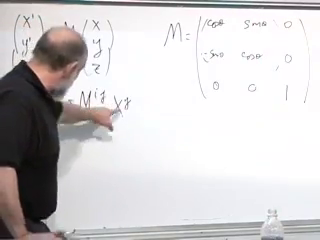
\includegraphics[width=0.82\textwidth]{lecture_05_figure_03.png}
\caption{Пространственный поворот, записанный и как матричное уравнение, и в индексной форме.}
\lectureframe{01:00:40}
\end{figure}

\section{Матрицы Лоренца и сложение скоростей}

Для движения вдоль \(x\) лоренцево преобразование в единицах \(c=1\) имеет вид
\begin{align}
x'&=\gamma_v(x-vt), & y'&=y,\nonumber\\
z'&=z, & t'&=\gamma_v(t-vx),
\end{align}
где
\begin{equation}
\gamma_v=\frac{1}{\sqrt{1-v^2}}.
\end{equation}
При порядке компонент \((x,y,z,t)\) это принимает вид
\begin{equation}
\begin{pmatrix}x'\\y'\\z'\\t'\end{pmatrix}
=
\begin{pmatrix}
\gamma_v&0&0&-\gamma_vv\\
0&1&0&0\\
0&0&1&0\\
-\gamma_vv&0&0&\gamma_v
\end{pmatrix}
\begin{pmatrix}x\\y\\z\\t\end{pmatrix}.
\label{eq:l5-lorentz-matrix}
\end{equation}

\begin{figure}[H]
\centering
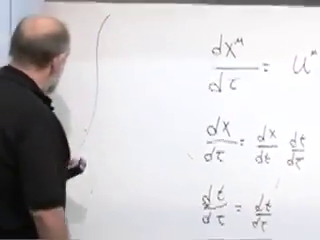
\includegraphics[width=0.82\textwidth]{lecture_05_figure_04.png}
\caption{Матрица Лоренца \(4\times4\). Смешиваются только компоненты \(x\) и \(t\); \(y\) и \(z\) остаются неизменными.}
\lectureframe{01:04:40}
\end{figure}

Теперь матричное умножение позволяет ответить на физический вопрос. Предположим, что один наблюдатель движется со скоростью \(v\) относительно нас, а третий — со скоростью \(u\) относительно него, причём все движутся вдоль одной и той же оси. Ньютоновская кинематика дала бы \(w=u+v\), что позволяло бы двум скоростям по \(3c/4\) сложиться в \(3c/2\). Теория относительности должна давать другое правило.

Нетривиальная часть буста — это матрица \(2\times2\)
\begin{equation}
B(v)=\gamma_v
\begin{pmatrix}1&-v\\-v&1\end{pmatrix}.
\end{equation}
Композиция двух бустов даёт
\begin{align}
B(u)B(v)
&=\gamma_u\gamma_v
\begin{pmatrix}1&-u\\-u&1\end{pmatrix}
\begin{pmatrix}1&-v\\-v&1\end{pmatrix}\nonumber\\
&=\gamma_u\gamma_v
\begin{pmatrix}
1+uv&-(u+v)\\
-(u+v)&1+uv
\end{pmatrix}.
\label{eq:l5-composed-boost}
\end{align}
Отношение внедиагонального элемента к диагональному определяет скорость результирующего буста:
\begin{equation}
w=\frac{u+v}{1+uv}
\qquad(c=1).
\end{equation}
Восстанавливая размерности,
\begin{equation}
w=\frac{u+v}{1+uv/c^2}.
\label{eq:l5-velocity-addition}
\end{equation}

\begin{figure}[H]
\centering
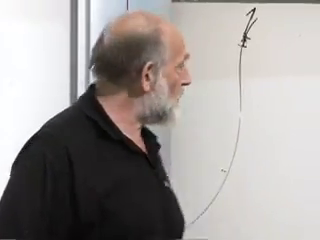
\includegraphics[width=0.82\textwidth]{lecture_05_figure_05.png}
\caption{Матрица композиции бустов и скорость
\(w=(u+v)/(1+uv)\) в естественных единицах.}
\lectureframe{01:15:35}
\end{figure}

Если \(u\) и \(v\) каждая близка к \(c\), числитель стремится к \(2c\), а знаменатель — к \(2\), так что \(w\) стремится к \(c\), а не к \(2c\). В более общем виде Eq.~\eqref{eq:l5-velocity-addition} отображает досветовые значения в досветовой результат. Матричное умножение автоматически закодировало предел скорости.

\section{Четырёхвекторы и непригодность обычной скорости}

Четырёхвектор — это любой объект, четыре компоненты которого преобразуются при поворотах и бустах Лоренца так же, как координаты пространства-времени. Если \(V^\mu\) — четырёхвектор, то при нашем соглашении о знаках
\begin{equation}
V_\mu=(-V^1,-V^2,-V^3,V^0),
\end{equation}
а его инвариантная норма равна
\begin{equation}
V_\mu V^\mu=(V^0)^2-(V^1)^2-(V^2)^2-(V^3)^2.
\end{equation}
Для двух четырёхвекторов \(V^\mu\) и \(W^\mu\) свёртка
\begin{equation}
W_\mu V^\mu
=W^0V^0-W^1V^1-W^2V^2-W^3V^3
\end{equation}
также инвариантна. Компоненты меняются при переходе от одной системы отсчёта к другой; свёртка — нет.

Обычная скорость имеет только три компоненты,
\begin{equation}
\mathbf v=\left(\frac{dx}{dt},\frac{dy}{dt},\frac{dz}{dt}\right).
\end{equation}
Добавление \(dt/dt=1\) не делает из неё полезный четырёхвектор. Четвёртая компонента была бы тривиальной, и получившийся объект не преобразовывался бы линейно при преобразованиях Лоренца. Координатное время \(t\) меняется от одной системы отсчёта к другой, поэтому дифференцирование по \(t\) нарушает требуемый закон преобразования.

Собственное время решает эту проблему. Вдоль мировой линии определим
\begin{equation}
u^\mu=\frac{dX^\mu}{d\tau}.
\label{eq:l5-four-velocity}
\end{equation}
Дифференциал \(dX^\mu\) является четырёхвектором, а величина \(d\tau\) инвариантна, поэтому их отношение — четырёхвектор. Прилагательное ``собственный'' относится к часам в знаменателе.

Правило цепочки связывает эту величину с обычной скоростью:
\begin{equation}
\frac{dx}{d\tau}=\frac{dx}{dt}\frac{dt}{d\tau},
\end{equation}
и аналогично для \(y\) и \(z\). Из уравнения~\eqref{eq:l5-proper-time},
\begin{align}
\left(\frac{d\tau}{dt}\right)^2
&=1-\left(\frac{dx}{dt}\right)^2
    -\left(\frac{dy}{dt}\right)^2
    -\left(\frac{dz}{dt}\right)^2\nonumber\\
&=1-v^2
\qquad(c=1),
\end{align}
и поэтому
\begin{equation}
\frac{dt}{d\tau}=\gamma_v=\frac{1}{\sqrt{1-v^2}}.
\end{equation}
Четыре компоненты имеют вид
\begin{equation}
u^i=\gamma_v v^i,
\qquad
u^0=\gamma_v
\qquad(c=1).
\label{eq:l5-four-velocity-components}
\end{equation}
При малой скорости \(u^i\simeq v^i\) и \(u^0\simeq1\). При скоростях, близких к скорости света,
\(\gamma_v\) неограниченно возрастает, и собственная скорость резко отличается от обычной.

\begin{figure}[H]
\centering
\includegraphics[width=0.82\textwidth]{lecture_05_figure_06.png}
\caption{Четыре компоненты собственной скорости, выраженные через обычную скорость и фактор Лоренца.}
\lectureframe{01:34:40}
\end{figure}

Восстанавливая обычные единицы и используя \(X^0=ct\), получаем стандартный вид
\begin{equation}
U^\mu=(\gamma_v\mathbf v,\gamma_v c)
\end{equation}
в используемом здесь порядке, где пространственные компоненты стоят первыми. Его инвариантная норма равна
\begin{equation}
U_\mu U^\mu=c^2.
\end{equation}
Следовательно, у любой массивной частицы модуль четырёхскорости имеет одно и то же инвариантное значение, хотя её пространственная скорость зависит от системы отсчёта.

\section{Касательный вектор к мировой линии}

Для уравнения~\eqref{eq:l5-four-velocity} есть знакомая евклидова модель. Вдоль кривой в обычном трёхмерном пространстве,
\begin{equation}
ds^2=dx^2+dy^2+dz^2.
\end{equation}
Дифференциальное смещение \((dx,dy,dz)\) направлено вдоль кривой, но не является единичным вектором. Деление на длину дуги даёт
\begin{equation}
\mathbf T=
\left(\frac{dx}{ds},\frac{dy}{ds},\frac{dz}{ds}\right),
\qquad
\mathbf T\cdot\mathbf T=1.
\end{equation}
Релятивистская конструкция — это та же идея, только с собственным временем вместо евклидовой длины дуги. Вектор \(u^\mu=dX^\mu/d\tau\) является касательным к мировой линии.

\begin{figure}[H]
\centering
\includegraphics[width=0.82\textwidth]{lecture_05_figure_07.png}
\caption{Евклидова конструкция касательного вектора: дифференциальное смещение делится на элемент длины дуги \(ds\). Собственное время играет аналогичную роль вдоль времеподобной мировой линии.}
\lectureframe{01:39:30}
\end{figure}

\begin{classroomqa}
\audiencequestion{Если \(c=1\), то собственное время и собственное расстояние — одно и то же?}
\lecturerresponse{Положив \(c=1\), мы выражаем время и расстояние в одних и тех же единицах; это не устраняет знаки минус в геометрии пространства-времени. В евклидовой аналогии \(s\) — это обычное расстояние, измеряемое вдоль пространственной кривой. Вдоль времеподобной мировой линии \(\tau\) — это прошедшее время, измеряемое часами. Конструкции аналогичны, но геометрии различны.}
\end{classroomqa}

Ещё одно дифференцирование определяет собственное ускорение,
\begin{equation}
a^\mu=\frac{du^\mu}{d\tau}.
\end{equation}
Именно эта величина должна заменить \(d^2\mathbf x/dt^2\), когда второму закону Ньютона придают релятивистскую форму. Поскольку величина \(u_\mu u^\mu\) постоянна,
\begin{equation}
\frac{d}{d\tau}(u_\mu u^\mu)=2u_\mu a^\mu=0,
\end{equation}
так что четырёхускорение ортогонально четырёхскорости относительно метрики Минковского.\editorialnote{Ортогональность немедленно следует из инвариантной нормы и включена как следующее математическое следствие определения.}

\section{Четырёхимпульс и энергия}

Импульс — наш последний пример, потому что он сохраняется при столкновениях и распадах. У частицы есть фиксированная присущая ей масса \(m\), которую часто называют массой покоя. Она не зависит от скорости. Релятивистский импульс равен произведению этой фиксированной массы на четырёхскорость:
\begin{equation}
p^\mu=mu^\mu.
\label{eq:l5-four-momentum}
\end{equation}
В единицах \(c=1\),
\begin{equation}
p^i=\gamma_v m v^i,
\qquad
p^0=\gamma_v m.
\end{equation}
При малой скорости \(\gamma_v\simeq1\), поэтому пространственные компоненты сводятся к ньютоновскому импульсу \(m\mathbf v\). При большой скорости они растут быстрее, чем \(m\mathbf v\).

Временная компонента — это энергия. В обычных единицах и при \(X^0=ct\),
\begin{equation}
P^\mu=(\mathbf p,E/c)
=(\gamma_v m\mathbf v,\gamma_v mc),
\end{equation}
и, следовательно,
\begin{equation}
E=\gamma_v mc^2
=mc^2\left(1-\frac{v^2}{c^2}\right)^{-1/2}.
\label{eq:l5-relativistic-energy}
\end{equation}

Чтобы вернуться к обычной механике, положим
\(\epsilon=v^2/c^2\ll1\). Биномиальное разложение даёт
\begin{equation}
(1-\epsilon)^p=1-p\epsilon+O(\epsilon^2).
\end{equation}
Подставляя \(p=-1/2\),
\begin{align}
E
&=mc^2\left(1-\frac{v^2}{c^2}\right)^{-1/2}\nonumber\\
&=mc^2\left[1+\frac12\frac{v^2}{c^2}
  +O\!\left(\frac{v^4}{c^4}\right)\right]\nonumber\\
&=mc^2+\frac12mv^2+O\!\left(\frac{mv^4}{c^2}\right).
\label{eq:l5-energy-expansion}
\end{align}

\begin{figure}[H]
\centering
\includegraphics[width=0.82\textwidth]{lecture_05_figure_08.png}
\caption{Разложение релятивистской энергии по малой скорости, выявляющее энергию покоя и ньютоновскую кинетическую энергию.}
\lectureframe{01:51:30}
\end{figure}

Первый член, \(mc^2\), присутствует даже в покое. В ньютоновской задаче с фиксированным набором частиц и неизменными массами этот член добавляет одну и ту же константу до и после движения, поэтому для привычного учёта имеет значение только \(\tfrac12mv^2\). Теория относительности показывает, что отброшенная константа всё это время была физической энергией.

Следовательно, энергия и импульс — не два несвязанных закона сохранения. Они являются четырьмя компонентами одного сохраняющегося вектора. Буст Лоренца смешивает их: то, что один наблюдатель называет энергией, частично входит в импульс другого наблюдателя, и наоборот. Тем не менее для изолированной системы полный четырёхимпульс одинаков до и после каждого столкновения или распада в любой инерциальной системе отсчёта.

Это порог релятивистской механики. Следующие задачи — выразить силу через собственное ускорение и понять релятивистские волновые уравнения, особенно уравнения, описывающие электромагнетизм и свет.

\chapter{Инвариантные законы, четырёхвекторы и тензор поля}

Мы начнём с закона, которому природа могла бы подчиняться, но не подчиняется. Его несостоятельность подскажет нам, как следует записывать физический закон. Тот же критерий сначала ведёт от координатных компонент к обычным векторам, затем от обычных векторов к четырёхвекторам и, наконец, от четырёхвекторов к тензорам. К концу обсуждения электрическое и магнитное поля уже не будут отдельными объектами: вместе они займут шесть независимых компонент одного антисимметричного тензора.

Если не оговорено иное, мы используем единицы, в которых \(c=1\), упорядочиваем компоненты пространства-времени как \((1,2,3,0)=(x,y,z,t)\) и используем сигнатуру метрики \((-,-,-,+)\).

\section{Возможный закон с неправильной симметрией}

Жёстко закрепим в пространстве оси \(x\) и \(y\). Теперь постулируем, что две частицы взаимодействуют всякий раз, когда совпадают их \(x\)-координаты. Взаимодействие может обратить их движение или отбросить их в новых направлениях; его детальная динамика несущественна. Предлагаемое условие срабатывания просто таково:
\begin{equation}
  x_1-x_2=0,
\end{equation}
где нижние индексы обозначают частицы, а не компоненты координат. В этом правиле нет никакого математического противоречия. Вопрос в том, что делает его физически неправдоподобным.

\begin{classroomqa}
\audiencequestion{Нарушает ли это правило однородность пространства?}
\lecturerresponse{Нет. Перенос начала координат изменяет обе координаты на одну и ту же величину и оставляет \(x_1-x_2\) неизменным. Правило не задаёт никакого предпочтительного места. Его недостаток связан с изотропией: оно выделяет одно предпочтительное направление.}
\end{classroomqa}

Повернём оси на \(90^\circ\). Старое направление \(x\) теперь называется \(y\), так что те же физические события описывались бы равенством \(y\)-координат. При произвольном угле условие включало бы линейную комбинацию \(x\) и \(y\). Следовательно, форма закона зависит от того, как была ориентирована доска. Он инвариантен относительно переносов, но не инвариантен относительно вращений.

Обычно мы придаём физическим законам их наиболее простой вид в ортогональных координатах. Можно пользоваться и более общими координатами, но тогда метрика и формулы становятся менее простыми. В классе ортогональных декартовых систем отсчёта никакая ориентация не должна быть привилегированной.

Исправление напрашивается сразу. В двумерном случае нужно требовать совпадения обеих координат; в трёхмерном случае — всех трёх:
\begin{equation}
  x_1=x_2,
  \qquad y_1=y_2,
  \qquad z_1=z_2.
\end{equation}
Тогда частицы могут взаимодействовать только тогда, когда достигают одной и той же точки, даже если они подходят к ней по разным линиям.

\begin{classroomqa}
\audiencequestion{Должны ли также совпадать \(z\)-координаты и времена?}
\lecturerresponse{В трёхмерном пространстве должны совпадать и \(z\)-координаты. Время пока опускается; мы вернём его, как только пространственный аргумент будет завершён.}
\end{classroomqa}

Пусть \(\boldsymbol r_a\) — положение частицы \(a\). Три покомпонентных условия превращаются в одно векторное уравнение,
\begin{equation}
  \boldsymbol r_1-\boldsymbol r_2=\boldsymbol 0.
\end{equation}
Компонента может обращаться в нуль в одной повёрнутой системе координат и не обращаться в нуль в другой. С целым вектором дело обстоит иначе: если в одной системе координат каждая компонента равна нулю, то и в любой повёрнутой системе координат каждая компонента равна нулю. Точно так же, если два вектора равны в одной системе координат, они остаются равными после преобразования обоих.

\begin{figure}[H]
\centering
\includegraphics[width=0.78\textwidth]{lecture_06_figure_01.png}
\caption{Три равенства координат, благодаря которым столкновение означает пространственное совпадение, а не совпадение вдоль одной предпочтительной оси.}
\lectureframe{00:09:00}
\end{figure}

Вот почему векторные уравнения полезны. Их компоненты меняются, но сам объект преобразуется согласованно. Закон, записанный для полного объекта, может сохранять свою форму при повороте координат.

\section{Совпадение в пространстве-времени}

Теперь заменим вертикальную пространственную ось временем. Ньютоновское правило могло бы утверждать, что два изменения движения происходят только при равных временах. В ньютоновской механике одновременность обща для всех инерциальных наблюдателей, так что такое правило возможно. В специальной теории относительности оно выделяет предпочтительную систему отсчёта. События, одновременные в одной системе отсчёта, не обязаны быть одновременными в другой.

Требовать совпадения только пространственных координат ничуть не лучше. Смещение в пространстве-времени может иметь нулевые пространственные компоненты и ненулевую временную компоненту,
\begin{equation}
  \Delta X^\mu=(0,0,0,\Delta t),
\end{equation}
а буст смешивает \(\Delta t\) с пространственной компонентой. Инвариантная локальная формулировка состоит в том, что два изменения движения происходят в одном и том же событии. Следовательно, простое столкновение требует
\begin{equation}
  X_1^\mu=X_2^\mu,
  \qquad\text{or}\qquad
  X_1^\mu-X_2^\mu=0.
\end{equation}
Совпадают все четыре координаты: частицы занимают одно и то же место в одно и то же время.

Пример со столкновением даёт общее правило записи физики. Мы можем перенести всё в одну сторону и приравнять полный четырёхвектор нулю либо приравнять один полный четырёхвектор другому. Приравнивание друг другу разрозненных частей четырёхвектора само по себе не даёт лоренц-инвариантного утверждения.

\section{Бусты, повороты и матричная запись}

Четырёхвектор — это объект, который преобразуется так же, как смещение в пространстве-времени. Чтобы сделать это определение полезным, сначала вспомним преобразования самих координат. Для буста со скоростью \(v\) в направлении \(x\) имеем
\begin{align}
  x'&=\gamma(x-vt), & y'&=y, & z'&=z,
  & t'&=\gamma(t-vx),                                      \label{eq:l6-boost}
\end{align}
где
\begin{equation}
  \gamma(v)=\frac{1}{\sqrt{1-v^2}}.
\end{equation}

\begin{classroomqa}
\audiencequestion{Положена ли в этих формулах скорость света равной единице?}
\lecturerresponse{Да. Если восстановить единицы, нужно взять \(X^0=ct\), заменить \(1-v^2\) на \(1-v^2/c^2\) и восстановить соответствующие множители \(c\) в смешанных пространственно--временных членах.}
\end{classroomqa}

Поворот вокруг оси \(z\) смешивает \(x\) и \(y\), оставляя \(z\) и \(t\) без изменения:
\begin{equation}
\begin{pmatrix}
  x'\\ y'\\ z'\\ t'
\end{pmatrix}
=
\begin{pmatrix}
  \cos\theta & \sin\theta & 0 & 0\\
  -\sin\theta & \cos\theta & 0 & 0\\
  0 & 0 & 1 & 0\\
  0 & 0 & 0 & 1
\end{pmatrix}
\begin{pmatrix}
  x\\ y\\ z\\ t
\end{pmatrix}.
\end{equation}
Нули полезно выписать: они явно показывают, какие компоненты не входят в данную преобразованную координату. В том же порядке буст из уравнения~\eqref{eq:l6-boost} имеет вид
\begin{equation}
\begin{pmatrix}
  x'\\ y'\\ z'\\ t'
\end{pmatrix}
=
\begin{pmatrix}
  \gamma & 0 & 0 & -\gamma v\\
  0 & 1 & 0 & 0\\
  0 & 0 & 1 & 0\\
  -\gamma v & 0 & 0 & \gamma
\end{pmatrix}
\begin{pmatrix}
  x\\ y\\ z\\ t
\end{pmatrix}.
\end{equation}

Повороты и бусты можно составлять с помощью умножения матриц. Чтобы выполнить буст в направлении, не совпадающем с исходной осью \(x\), можно повернуть это направление к оси \(x\), применить буст и затем повернуть как нужно. Произведения этих элементарных матриц порождают более общие преобразования Лоренца.

\begin{classroomqa}
\audiencequestion{Имеет ли значение, сначала выполнять поворот, а потом буст, или сначала буст, а потом поворот?}
\lecturerresponse{Да. После первой операции оси, относительно которых действует вторая, уже изменились. Эти два произведения матриц могут не совпадать, так что порядок операций имеет значение.}
\end{classroomqa}

Все эти линейные преобразования можно сразу записать как
\begin{equation}
  X'^{\mu}=\Lambda^{\mu}{}_{\nu}X^{\nu}.                  \label{eq:l6-vector-transform}
\end{equation}
Повторяющийся индекс \(\nu\) суммируется по \(1,2,3,0\). Это просто обычная сумма произведений элементов строки и столбца при умножении матриц, записанная в индексной форме.

\begin{figure}[H]
\centering
\includegraphics[width=0.78\textwidth]{lecture_06_figure_02.png}
\caption{Лоренцево преобразование в индексной записи над началом его записи через вектор-столбец.}
\lectureframe{00:31:55}
\end{figure}

Уравнение~\eqref{eq:l6-vector-transform} также служит определением общего контравариантного четырёхвектора. Если \(A^\mu\) — такой вектор, то
\begin{equation}
  A'^{\mu}=\Lambda^{\mu}{}_{\nu}A^{\nu}.
\end{equation}
Его четыре компоненты не обязаны представлять положение. То, что делает объект четырёхвектором, — это закон его преобразования.

\section{Скаляры, метрика и инвариантные произведения}

Прежде чем использовать дополнительные четырёхвекторы, полезно вернуться к более простому понятию скаляра. При пространственных вращениях температура в заданной точке является скаляром, как и расстояние между двумя заданными точками. Каждая из этих величин представляет собой одно число, не зависящее от ориентации осей. Можно даже сделать нарочито нелепое численное утверждение, что расстояние, измеренное в сантиметрах, равно температуре комнаты, измеренной в градусах Фаренгейта. Это утверждение лишено физической глубины, но, поскольку обе стороны — скаляры относительно вращений, его истинность или ложность не зависит от того, как повёрнуты оси.

Компоненты вектора не являются скалярами. Поэтому нам нужен систематический способ объединять их в скаляры. Запишем общий контравариантный четырёхвектор как
\begin{equation}
  A^\mu=(A^1,A^2,A^3,A^0).
\end{equation}
Ковариантные компоненты описывают тот же геометрический объект, но с нижним индексом. При нашей сигнатуре они получаются с помощью метрики Минковского,
\begin{equation}
  A_\mu=\eta_{\mu\nu}A^\nu,
  \qquad
  \eta_{\mu\nu}=
  \begin{pmatrix}
    -1&0&0&0\\
    0&-1&0&0\\
    0&0&-1&0\\
    0&0&0&1
  \end{pmatrix},                                          \label{eq:l6-metric}
\end{equation}
так что
\begin{equation}
  A_\mu=(-A^1,-A^2,-A^3,A^0).
\end{equation}

\begin{classroomqa}
\audiencequestion{Есть ли на доске несогласованность в двух индексах и знаках?}
\lecturerresponse{Да. Пространственной компоненте в выписанном столбце нужен соответствующий минус, а компоненты справа в уравнении понижения индекса до умножения на \(\eta_{\mu\nu}\) должны нести верхние индексы. Временная метка — \(0\), а не \(4\).}
\end{classroomqa}

\begin{figure}[H]
\centering
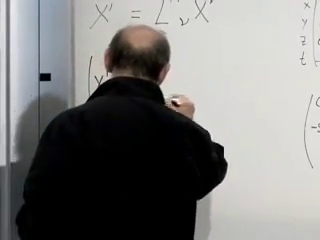
\includegraphics[width=0.8\textwidth]{lecture_06_figure_03.png}
\caption{Контравариантные и ковариантные компоненты, матрица метрики и начало инвариантной свёртки.}
\lectureframe{00:45:00}
\end{figure}

Понижение индекса — не украшение. Оно собирает знаки, необходимые для лоренц-инвариантной нормы:
\begin{align}
  A_\mu A^\mu
  &=-(A^1)^2-(A^2)^2-(A^3)^2+(A^0)^2,                    \label{eq:l6-norm}\\
  X_\mu X^\mu
  &=t^2-x^2-y^2-z^2.
\end{align}
Второе выражение есть инвариантный интервал пространства-времени от начала координат. Поскольку \(A^\mu\) преобразуется так же, как \(X^\mu\), его свёртка обладает той же инвариантностью.

Эта запись также подсказывает полезное правило учёта. Повторяющийся индекс суммирования встречается один раз вверху и один раз внизу. Например,
\begin{equation}
  A_\mu A^\mu
  =\eta_{\mu\nu}A^\mu A^\nu.
\end{equation}
Обозначения суммируемых, или фиктивных, индексов можно менять, не изменяя самой величины.

\begin{classroomqa}
\audiencequestion{Следует ли считать один из этих векторов строкой, а другой столбцом, и имеет ли значение их порядок?}
\lecturerresponse{В данном вычислении рассматривайте индексированные величины как компоненты и предоставьте метрике выполнить свёртку; нет нужды превращать обсуждение в операторную алгебру строк и столбцов. Это обычные числа, поэтому их порядок не имеет значения. Для некоммутирующих операторов потребовалась бы бо́льшая осторожность, но здесь речь не об этом.}
\end{classroomqa}

Та же конструкция задаёт скалярное произведение двух различных четырёхвекторов,
\begin{equation}
  A\mathbin{\cdot}B=A_\mu B^\mu=A^\mu B_\mu.
\end{equation}
Его инвариантность следует без явной записи матрицы Лоренца. Поскольку \(A+B\) и \(A-B\) являются четырёхвекторами, оба квадрата их норм инвариантны:
\begin{align}
  (A+B)^2&=A^2+B^2+2A\mathbin{\cdot}B,\\
  (A-B)^2&=A^2+B^2-2A\mathbin{\cdot}B.
\end{align}
Вычитая, получаем
\begin{equation}
  (A+B)^2-(A-B)^2=4A\mathbin{\cdot}B,                    \label{eq:l6-polarization}
\end{equation}
поэтому \(A\mathbin{\cdot}B\) тоже инвариантно. Множитель четыре следует непосредственно из разложения.\editorialnote{Вывод у доски даёт это поляризационное тождество; явная запись множителя делает озвученное сокращение недвусмысленным.}

\begin{figure}[H]
\centering
\includegraphics[width=0.8\textwidth]{lecture_06_figure_04.png}
\caption{Два инвариантных квадрата, используемые для выделения скалярного произведения различных четырёхвекторов.}
\lectureframe{00:52:20}
\end{figure}

Инвариантные величины естественно входят в физические законы: в отличие от отдельной компоненты, они сохраняют одно и то же значение при переходе от одной системы отсчёта к другой.

\section{Собственная скорость и четырёхимпульс}

Рассмотрим два соседних события на мировой линии частицы. Их разделяет бесконечно малый четырёхвектор
\begin{equation}
  dX^\mu=(dx,dy,dz,dt).
\end{equation}
Для времениподобной мировой линии собственное время определяется как
\begin{equation}
  d\tau^2=dX_\mu dX^\mu
  =dt^2-dx^2-dy^2-dz^2.                                  \label{eq:l6-proper-time}
\end{equation}
Собственная четырёхскорость равна
\begin{equation}
  U^\mu=\frac{dX^\mu}{d\tau}.                            \label{eq:l6-four-velocity}
\end{equation}
Она измеряет скорость изменения положения в пространстве-времени по собственному времени самой частицы, а не по координатному времени выбранной системы отсчёта.

Хотя \(U^\mu\) имеет четыре компоненты, независимы только три. Разделив ~\eqref{eq:l6-proper-time} на \(d\tau^2\), получаем
\begin{equation}
  U_\mu U^\mu=1.
\end{equation}
Следовательно, четырёхскорость является единичным времениподобным вектором. Выбор направления в будущее фиксирует знак её временной компоненты.

\begin{classroomqa}
\audiencequestion{При скоростях, много меньших \(c\), сводится ли четырёхскорость к обычной скорости?}
\lecturerresponse{Её три пространственные компоненты стремятся к обычной скорости, тогда как временная компонента стремится к единице в единицах \(c=1\). Это соотношение следует из применения правила дифференцирования сложной функции и вычисления \(dt/d\tau\).}
\end{classroomqa}

Для каждой пространственной компоненты
\begin{equation}
  U^i=\frac{dx^i}{d\tau}
     =\frac{dx^i}{dt}\frac{dt}{d\tau}
     =v^i\frac{dt}{d\tau}.
\end{equation}
Разделим ~\eqref{eq:l6-proper-time} на \(dt^2\):
\begin{equation}
  \left(\frac{d\tau}{dt}\right)^2
  =1-v_x^2-v_y^2-v_z^2
  =1-\boldsymbol v^2.
\end{equation}
Следовательно,
\begin{equation}
  \frac{dt}{d\tau}=\frac{1}{\sqrt{1-\boldsymbol v^2}}
  =\gamma(\lvert\boldsymbol v\rvert),
\end{equation}
и
\begin{equation}
  U^\mu=(\gamma v_x,\gamma v_y,\gamma v_z,\gamma).
                                                                  \label{eq:l6-u-components}
\end{equation}

\begin{figure}[H]
\centering
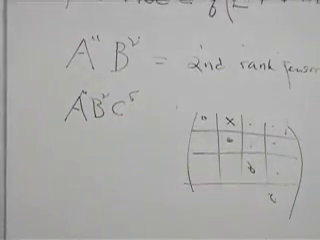
\includegraphics[width=0.8\textwidth]{lecture_06_figure_05.png}
\caption{Вычисление собственного времени, которое даёт \(dt/d\tau=\gamma\) и связывает собственную скорость с обычной скоростью.}
\lectureframe{01:02:00}
\end{figure}

\begin{classroomqa}
\audiencequestion{Означает ли \(dx^2/dt^2\) вторую производную, и должны ли при возведении вектора в квадрат возникать перекрёстные члены?}
\lecturerresponse{Здесь это означает \((dx/dt)^2\), квадрат первой производной. Кроме того, \(\boldsymbol v^2\) означает евклидово скалярное произведение \(v_x^2+v_y^2+v_z^2\), а не квадрат формальной суммы \(v_x+v_y+v_z\); перекрёстных членов нет.}
\end{classroomqa}

\begin{classroomqa}
\audiencequestion{Является ли \(v\) в \(\gamma(v)\) относительной скоростью двух систем отсчёта или скоростью частицы?}
\lecturerresponse{Здесь это скорость частицы в выбранной системе отсчёта. Функцию \(\gamma(v)=1/\sqrt{1-v^2}\) можно вычислять для любой скорости: при бусте она вычисляется на относительной скорости систем отсчёта; в четырёхскорости — на скорости частицы.}
\end{classroomqa}

Для \(v\ll1\), \(\gamma\simeq1\), поэтому пространственные компоненты \(U^\mu\) стремятся к \(\boldsymbol v\), а \(U^0\) стремится к единице. Когда обычная скорость приближается к скорости света, \(\gamma\) и все ненулевые компоненты четырёхскорости растут без ограничения.

\begin{classroomqa}
\audiencequestion{Не должна ли \(U^0\) иметь размерность скорости, вместо того чтобы быть близкой к числу один?}
\lecturerresponse{Размерности исчезли, когда \(c\) было положено равным единице. При \(X^0=ct\) имеем
\(U^\mu=(\gamma\boldsymbol v,\gamma c)\), так что временная компонента стремится к \(c\), и \(U_\mu U^\mu=c^2\).}
\end{classroomqa}

Для частицы с массой покоя \(m\) определим четырёхимпульс как
\begin{equation}
  P^\mu=mU^\mu.
\end{equation}
В естественных единицах
\begin{equation}
  P^\mu=(\gamma m\boldsymbol v,\gamma m).
\end{equation}
Первые три компоненты при малой скорости стремятся к ньютоновскому импульсу \(m\boldsymbol v\). Восстанавливая единицы, получаем
\begin{equation}
  P^\mu=(\gamma m\boldsymbol v,E/c),
  \qquad E=\gamma mc^2,
\end{equation}
и, следовательно,
\begin{equation}
  E=mc^2+\frac{1}{2}m\boldsymbol v^2+O(mv^4/c^2).
\end{equation}
Временная компонента есть энергия в единицах \(c=1\) или энергия, делённая на \(c\), когда всем четырём компонентам приписываются единицы импульса.

\begin{classroomqa}
\audiencequestion{Является ли обычная \(\boldsymbol v\), если дописать к ней четвёртую компоненту, сама по себе четырёхвектором?}
\lecturerresponse{Нет. Обычная трёхскорость не преобразуется как четырёхвектор. Множитель \(\gamma\) и определение через собственное время существенны; четырёхвектор — это \(U^\mu\), а не \(\boldsymbol v\).}
\end{classroomqa}

\section{Почему электрическое и магнитное поля должны смешиваться}

Теперь вернёмся к тому, что было названо кратким отпуском от относительности. Начнём с доэйнштейновского уравнения движения и спросим, как его нужно перестроить, чтобы оно могло быть справедливым в любой инерциальной системе отсчёта. Обычное ускорение есть производная обычной скорости по времени. Его четырёхмерным аналогом естественно является
\begin{equation}
  A^\mu=\frac{dU^\mu}{d\tau}.
\end{equation}
При малой скорости его пространственные компоненты стремятся к обычному ускорению. Полное релятивистское уравнение будет отложено; сначала рассмотрим старый закон силы.

Для заряда \(q\) в электрическом и магнитном полях
\begin{equation}
  \boldsymbol F=m\boldsymbol a
  =q\left(\boldsymbol E+\boldsymbol v\times\boldsymbol B\right).
                                                                  \label{eq:l6-lorentz-force}
\end{equation}
Электрический член не зависит от скорости частицы, тогда как магнитный зависит.

\begin{figure}[H]
\centering
\includegraphics[width=0.8\textwidth]{lecture_06_figure_06.png}
\caption{Дорелятивистская форма закона силы Лоренца, которая мотивирует объединение \(\boldsymbol E\) и \(\boldsymbol B\).}
\lectureframe{01:18:20}
\end{figure}

Предположим, наблюдатель не видит электрического поля, но видит магнитное поле и движущийся заряд. Заряд испытывает магнитную силу. Однако в мгновенной системе покоя заряда \(\boldsymbol v=0\), поэтому магнитный член в ~\eqref{eq:l6-lorentz-force} обращается в нуль. Физическая мировая линия не стала инерциальной лишь потому, что изменились координаты; следовательно, сила в новой системе должна включать электрический вклад. Точнее, ненулевое четырёхускорение нельзя преобразованием между инерциальными системами обратить в нуль, хотя трёхускорение и его компоненты преобразуются.
\editorialnote{Это утверждение о четырёхускорении является инвариантной формой аудиторного аргумента и позволяет не трактовать обычное трёхускорение само по себе как инвариант относительно системы отсчёта.}

Следовательно, электрическое и магнитное поля должны преобразовываться друг в друга. Вместе у них шесть компонент, поэтому они не являются ни одним скаляром, ни одним четырёхвектором. Нам нужен новый объект с собственным законом преобразования.

\section{Тензоры: по одному преобразованию на индекс}

Скаляр можно назвать тензором ранга нуль; у него нет индексов. Четырёхвектор — тензор ранга один; у него один индекс с четырьмя возможными значениями. Простейший пример ранга два — произведение
\begin{equation}
  A^\mu B^\nu.
\end{equation}
Каждый индекс принимает четыре значения, поэтому у объекта \(4^2=16\) компонент, которые можно представить в виде массива \(4\times4\). Произведение трёх векторов,
\begin{equation}
  A^\mu B^\nu C^\sigma,
\end{equation}
имеет \(4^3=64\) компонент и является тензором ранга три. Для более высоких рангов схема продолжается. Название менее важно, чем правило, которым определяется объект.

Если
\begin{equation}
  A'^{\mu}=\Lambda^\mu{}_{\nu}A^\nu,
  \qquad
  B'^{\sigma}=\Lambda^\sigma{}_{\tau}B^\tau,
\end{equation}
то их произведение преобразуется как
\begin{equation}
  A'^{\mu}B'^{\sigma}
  =\Lambda^\mu{}_{\nu}\Lambda^\sigma{}_{\tau}
   A^\nu B^\tau.
\end{equation}
Это даёт определяющий закон для контравариантного тензора ранга два:
\begin{equation}
  T'^{\mu\sigma}
  =\Lambda^\mu{}_{\nu}\Lambda^\sigma{}_{\tau}T^{\nu\tau}.
                                                                  \label{eq:l6-tensor-transform}
\end{equation}
Каждому индексу соответствует одна матрица Лоренца. Повторяющиеся \(\nu\) и \(\tau\) суммируются; свободные \(\mu\) и \(\sigma\) обозначают компоненту, вычисляемую в штрихованной системе отсчёта.

\begin{figure}[H]
\centering
\includegraphics[width=0.82\textwidth]{lecture_06_figure_07.png}
\caption{Преобразование двух векторов и вытекающий из него двухматричный закон преобразования тензора ранга два.}
\lectureframe{01:27:15}
\end{figure}

Тензор не обязан быть одиночным произведением векторов. И \(A^\mu B^\nu\), и \(A^\nu B^\mu\) подчиняются тензорному закону преобразования, как и их сумма и любая сумма вида
\begin{equation}
  A^\mu B^\nu+C^\mu D^\nu.
\end{equation}
Определением служит закон преобразования, а не конкретная факторизация. Тензор третьего ранга получает третью матрицу Лоренца, и так далее.

\section{Симметричные и антисимметричные тензоры}

Два класса тензоров ранга два будут особенно полезны. Симметричный тензор удовлетворяет
\begin{equation}
  T^{\mu\nu}=T^{\nu\mu},
\end{equation}
так что элементы, отражённые относительно диагонали, совпадают. Его четыре диагональных элемента и шесть элементов по одну сторону диагонали определяют остальные, давая
\begin{equation}
  4+6=10
\end{equation}
независимых компонент.

Антисимметричный тензор удовлетворяет
\begin{equation}
  T^{\mu\nu}=-T^{\nu\mu}.                                \label{eq:l6-antisymmetry}
\end{equation}
Подстановка \(\mu=\nu\) в ~\eqref{eq:l6-antisymmetry} даёт
\(T^{\mu\mu}=-T^{\mu\mu}\), так что каждый диагональный элемент равен нулю. Шесть элементов в одной треугольной половине определяют остальные шесть изменением знака. Поэтому имеется ровно шесть независимых компонент.

\begin{figure}[H]
\centering
\includegraphics[width=0.82\textwidth]{lecture_06_figure_08.png}
\caption{Заполненный антисимметричный массив \(4\times4\): нули на диагонали и противоположные знаки по разные стороны от неё.}
\lectureframe{01:34:25}
\end{figure}

Именно это число и служит подсказкой. Три электрические и три магнитные компоненты могут поместиться в один антисимметричный тензор ранга два.

\section{Тензор электромагнитного поля}

Пусть метки пространства-времени идут по строкам и столбцам в порядке
\((1,2,3,0)=(x,y,z,t)\). Запись на доске имеет вид
\begin{equation}
  F_{\mu\nu}=
  \begin{pmatrix}
    0    & -B_3 & B_2  & E_1\\
    B_3  & 0    & -B_1 & E_2\\
    -B_2 & B_1  & 0    & E_3\\
    -E_1 & -E_2 & -E_3 & 0
  \end{pmatrix}.                                         \label{eq:l6-field-tensor}
\end{equation}
Чисто пространственные ячейки содержат магнитное поле; ячейки с одним пространственным и одним временным индексом содержат электрическое поле. Антисимметрия задаёт элементы нижнего треугольника, как только известны элементы верхнего треугольника.

\begin{classroomqa}
\audiencequestion{Все ли магнитные элементы отрицательны, и соответствуют ли метки \(x,y,z\)?}
\lecturerresponse{Знаки в верхнем пространственном треугольнике чередуются так, как показано: \(-B_3,+B_2,-B_1\). Метки \(1,2,3\) соответствуют \(x,y,z\), тогда как \(0\) обозначает время. При отражении относительно диагонали каждый знак меняется на противоположный.}
\end{classroomqa}

\begin{figure}[H]
\centering
\includegraphics[width=0.82\textwidth]{lecture_06_figure_09.png}
\caption{Полный тензор электромагнитного поля в используемом в лекции порядке компонент, где пространственные компоненты идут первыми.}
\lectureframe{01:41:05}
\end{figure}

Обозначение по соглашению пишут как \(F_{\mu\nu}\), а не как общее
\(T_{\mu\nu}\). Лектор предполагает, что буква может отсылать к
Фарадею, одновременно прямо говоря, что не знает истории этого
обозначения. Здесь важны его антисимметрия и шесть компонентов поля,
а не это предположение о букве.

\begin{classroomqa}
\audiencequestion{Представляет ли каждый элемент матрицы величину поля в указанной координатной плоскости?}
\lecturerresponse{Это компонента тензора электромагнитного поля.
Элементы, содержащие время, являются электрическими компонентами, а пространственные--пространственные
элементы кодируют магнитные компоненты.}
\end{classroomqa}

Отделите строку и столбец, несущие временной индекс. Оставшийся
антисимметричный блок \(3\times3\) соответствует магнитному полю. Его независимые элементы удобно
запоминать циклически:
\begin{equation}
  F_{12}=-B_3,
  \qquad F_{23}=-B_1,
  \qquad F_{31}=-B_2.                                   \label{eq:l6-magnetic-cycle}
\end{equation}
Начиная с первого соотношения, циклически сдвигайте все метки по
\(1\to2\to3\to1\). Эквивалентно,
\begin{equation}
  F_{ij}=-\epsilon_{ijk}B_k,
\end{equation}
где \(\epsilon_{123}=+1\).\editorialnote{Формула Леви--Чивиты — компактная стандартная форма циклического правила, явно выведенного на доске.}

\begin{figure}[H]
\centering
\includegraphics[width=0.82\textwidth]{lecture_06_figure_10.png}
\caption{Циклические пространственные компоненты, кодирующие магнитное поле в антисимметричном тензоре.}
\lectureframe{01:46:20}
\end{figure}

Для электрического поля соответствия более прямые:
\begin{equation}
  E_1=F_{10},
  \qquad E_2=F_{20},
  \qquad E_3=F_{30}.
\end{equation}

Поэтому для магнитного поля полезны два отождествления. Внутри
трёхмерного пространства трёхкомпонентному аксиальному вектору можно
поставить в соответствие антисимметричный тензор \(3\times3\). В пространстве-времени,
однако, оно является лишь пространственной частью шестикомпонентного тензора
\(F_{\mu\nu}\). Такое сопоставление специфично для трёх измерений:
антисимметричный тензор \(4\times4\) имеет шесть независимых компонент и не
может быть отождествлён с четырёхвектором.
\editorialnote{При собственных вращениях магнитное поле ведёт себя как вектор;
при отражениях, точнее, как аксиальный вектор, или псевдовектор.}

Цель этой конструкции не в подсчёте компонент как таковом.
Поскольку \(F_{\mu\nu}\) преобразуется как тензор, буст Лоренца автоматически
смешивает его электрические и магнитные элементы. На следующей лекции его
можно будет объединить с четырёхскоростью и четырёхускорением, чтобы заменить
уравнение~\eqref{eq:l6-lorentz-force} ковариантным уравнением движения.

\section{Вопросы об Эйнштейне и Минковском}

В последние минуты разговор переходит от формализма к тому, как он возник исторически. Ответы даются как воспоминания, а не как установленная история, и эта оговорка сама является частью обсуждения.

\begin{classroomqa}
\audiencequestion{Искал ли Эйнштейн лоренц-инвариантную формулировку из концептуальных соображений, или его к ней вели конкретные наблюдения?}
\lecturerresponse{Принцип, согласно которому законы природы должны иметь одну и ту же форму во всякой инерциальной системе отсчёта, был центральным в его рассуждениях. Были также экспериментальные данные, касающиеся света и невозможности обнаружить движение сквозь эфир, хотя лектор прямо не уверен, какие именно результаты были известны Эйнштейну и насколько сильно они на него повлияли. Концептуальное требование состояло в том, что уравнения Максвелла и сила Лоренца должны подчиняться принципу относительности, а это требует, чтобы электрические поля, магнитные поля и компоненты скорости преобразовывались совместно.}
\end{classroomqa}

В изложении Эйнштейна 1905 года не использовалась компактная нотация четырёхвекторов,
используемая здесь. Там всё делалось покомпонентно, с явной записью необходимых
множителей \(\gamma\) и скорости. Минковский впоследствии организовал ту же
структуру геометрически как четырёхмерное пространство-время.

\begin{classroomqa}
\audiencequestion{Сопротивлялся ли Эйнштейн простран\-ственно-временной формулировке Минковского, и как скоро Минковский её ввёл?}
\lecturerresponse{Высказанное на занятии воспоминание состоит в том, что Эйнштейн поначалу не приветствовал четырёхмерный геометрический язык, но быстро оценил его ценность. Время указывается предположительно как примерно через два года после статьи 1905 года, возможно 1907; выступающий подчёркивает, что он вспоминает, а не устанавливает историю.}
\end{classroomqa}

\begin{classroomqa}
\audiencequestion{Был ли Минковский математиком или физиком, что ещё он внёс, и испытывал ли он влияние Лоренца или Фицджеральда?}
\lecturerresponse{Никакого уверенного ответа не даётся. Различие между математиком и физиком не разбиралось, поправка из аудитории прерывает общее замечание о других работах Минковского, а возможные линии влияния прямо оставляются неопределёнными. Надёжный пункт для этого обсуждения состоит в том, что Минковский решающим образом оформил теорию относительности в четырёхмерной геометрической нотации.}
\end{classroomqa}

\begin{classroomqa}
\audiencequestion{Присутствовали ли преобразования, смешивающие \(\boldsymbol E\) и
\(\boldsymbol B\), уже в работе Эйнштейна 1905 года?}
\lecturerresponse{Да, но они были записаны покомпонентно, а не как одно
уравнение полевого тензора. Проведённое на занятии сравнение — с покомпонентными
уравнениями Максвелла: содержание может присутствовать и до появления компактной
нотации, раскрывающей его общую структуру. Вклад Минковского состоял в том,
чтобы сделать эту структуру систематической на языке пространства-времени.}
\end{classroomqa}

Это возвращает нас к математической мысли, с которой мы начали. Компоненты незаменимы для вычислений, но закон становится понятным, когда эти компоненты распознаются как части единого преобразующегося объекта. Следующая задача — использовать \(F_{\mu\nu}\), чтобы записать уравнение движения заряженной частицы в форме, одинаковой во всех инерциальных системах отсчёта.

\chapter{Заряженные частицы, преобразования полей и релятивистские волны}

В прошлый раз мы начали выяснять, как движется заряженная частица в электрическом и магнитном полях, когда учитываются принципы теории относительности. Уже знакомый закон силы Лоренца содержит подсказку: его магнитный член зависит от скорости частицы, поэтому разные наблюдатели не могут по отдельности прийти к согласию о том, что является электрическим, а что магнитным. Наша задача — сформулировать этот закон так, чтобы каждый инерциальный наблюдатель пользовался одним и тем же уравнением, хотя поля и скорость частицы меняются при переходе от одной системы отсчета к другой.

Если не оговорено иное, мы используем единицы, в которых \(c=1\), а сигнатура метрики имеет вид \((-,-,-,+)\). Компоненты пространства-времени упорядочены так, что сначала идут три пространственные компоненты:
\begin{equation}
  \mu=(1,2,3,0)=(x,y,z,t).
\end{equation}
Латинские индексы \(m,n\) пробегают только три пространственных направления.

\section{Что остается от ньютоновского закона силы}

В ньютоновской механике
\begin{equation}
  \boldsymbol F=m\boldsymbol a
\end{equation}
имеет один и тот же вид во всех инерциальных системах отсчета, потому что галилеевы наблюдатели согласны относительно ускорения. Они также приписывают частице одну и ту же массу и одну и ту же силу. Как только кинематика меняется, нет оснований ожидать, что именно это соотношение между силой и обычным ускорением сохранится без изменений.

Электромагнетизм и гравитация уже предупреждают нас, что релятивистские обобщения не обязаны быть похожими друг на друга. Закон Кулона и ньютоновский закон тяготения оба являются законами обратных квадратов, но гравитацию нельзя естественным образом включить в специальную теорию относительности без более глубокого изменения геометрии пространства-времени. С электромагнетизмом это возможно. Более того, магнетизм сам по себе является релятивистским эффектом: когда множители \(c\) восстановлены, магнитная сила содержит множитель скорости, деленной на \(c\), и исчезает в формальном пределе \(c\to\infty\).

То, что в ньютоновском законе сохраняется, — это утверждение, что сила есть скорость изменения импульса. При постоянной массе покоя
\begin{equation}
  \boldsymbol F
  =m\frac{d\boldsymbol v}{dt}
  =\frac{d}{dt}(m\boldsymbol v)
  =\frac{d\boldsymbol p}{dt}.
\end{equation}
Теория относительности изменит связь между импульсом и скоростью, но сохранит этот способ организации уравнения.

\begin{figure}[H]
\centering
\includegraphics[width=0.64\textwidth]{lecture_07_figure_01.png}
\caption{Сила переписывается в виде \(d\boldsymbol p/dt\), в то время как на доске записывается электрическая часть закона Лоренца.}
\lectureframe{00:08:20}
\end{figure}

В единицах \(c=1\) дорелятивистский закон силы Лоренца имеет вид
\begin{equation}
  \frac{d\boldsymbol p}{dt}
  =q\bigl(\boldsymbol E+\boldsymbol v\times\boldsymbol B\bigr).
  \label{eq:lorentz-three}
\end{equation}
Оба поля могут зависеть от положения и времени. Нерелятивистский предел теперь есть предел \(v\ll 1\), а не предел, в котором числовая константа \(c=1\) каким-то образом меняется. Электрический член в \eqref{eq:lorentz-three} уже является обычным вектором. Чтобы понять магнитный член в форме, которую можно перенести в пространство-время, надо снова посмотреть на векторное произведение.

\section{Векторное произведение как антисимметричный тензор}

Возьмем два трехмерных вектора \(\boldsymbol A\) и \(\boldsymbol B\). Их внешнее произведение
\begin{equation}
  T_{mn}=A_mB_n
\end{equation}
является тензором ранга два с девятью компонентами. Вообще говоря, никакой симметрией он не обладает. Антисимметризация дает
\begin{equation}
  K_{mn}=A_mB_n-A_nB_m,
  \qquad K_{mn}=-K_{nm}.
  \label{eq:antisym-product}
\end{equation}
Его диагональные элементы равны нулю, а каждый элемент ниже диагонали определяется соответствующим элементом выше нее. Следовательно, антисимметричный тензор \(3\times3\) имеет только три независимые компоненты.

Этот подсчет наводит на мысль, но сам по себе недостаточен. Три величины не автоматически преобразуются как вектор. Однако в трех измерениях три независимых элемента \eqref{eq:antisym-product} можно отождествить с компонентами векторного произведения \(\boldsymbol C=\boldsymbol A\times\boldsymbol B\). Сначала на доске \(C_2\) временно помещается в правый верхний угол:

\begin{figure}[H]
\centering
\includegraphics[width=0.75\textwidth]{lecture_07_figure_02.png}
\caption{Антисимметричное произведение в тот момент, когда его три независимых элемента сопоставляются с компонентами \(\boldsymbol C\). Обозначение в правом верхнем углу здесь еще предварительное.}
\lectureframe{00:17:33}
\end{figure}

Циклическая перестановка \(1\to2\to3\to1\) дает формулы для компонент
\begin{align}
  C_3 &= A_1B_2-A_2B_1, \\
  C_1 &= A_2B_3-A_3B_2, \\
  C_2 &= A_3B_1-A_1B_3.
  \label{eq:cross-components}
\end{align}
Последняя строка показывает, что элемент в правом верхнем углу равен \(-C_2\), а не \(C_2\). Эта поправка составляет часть рассуждения, а не деталь, которую следует скрыть.

\begin{figure}[H]
\centering
\includegraphics[width=0.62\textwidth]{lecture_07_figure_03.png}
\caption{Завершенные циклические тождества для компонент, которые исправляют временный знак в антисимметричном массиве.}
\lectureframe{00:21:54}
\end{figure}

Получающаяся матрица имеет вид
\begin{equation}
  K_{mn}=
  \begin{pmatrix}
    0 & C_3 & -C_2 \\
    -C_3 & 0 & C_1 \\
    C_2 & -C_1 & 0
  \end{pmatrix}.
  \label{eq:cross-matrix}
\end{equation}

За этим обозначением стоит полезная геометрия. Компонента с индексами \(1,2\) естественным образом относится к плоскости \(xy\) и отождествляется с векторной компонентой вдоль перпендикулярной оси \(z\). Один и тот же ориентированный объект можно описывать либо плоскостью, либо стрелкой, нормальной к этой плоскости. Описание через стрелку специфично для трех измерений; в более высоких размерностях антисимметричный тензор ранга два по-прежнему существует, но число его компонент уже не совпадает с числом компонент вектора. Поэтому обобщается именно тензор, а не перпендикулярная стрелка.

Эквивалентно, после выбора ориентации,
\begin{equation}
  C_k=\frac12\epsilon_{kmn}K_{mn}.
\end{equation}
Необходимость выбрать ориентацию лежит в основе правила правой руки и привычного различия между полярными и аксиальными векторами.
\editorialnote{Формула Леви--Чивиты и терминология аксиальных векторов — это стандартные обозначения для геометрии, в которой сопоставляются плоскость и нормаль, явно развернутой в лекции.}

\section{Магнитное поле в тензорной форме}

То же двойственное описание применимо и к магнитному полю. Его антисимметричный пространственный тензор определим как
\begin{equation}
  B_{mn}=
  \begin{pmatrix}
    0 & -B_3 & B_2 \\
    B_3 & 0 & -B_1 \\
    -B_2 & B_1 & 0
  \end{pmatrix}.
  \label{eq:magnetic-tensor}
\end{equation}
Дополнительный общий знак по сравнению с \eqref{eq:cross-matrix} является соглашением. После того как он выбран, им нужно пользоваться последовательно; изменение знака у всех трех векторных компонент описывало бы то же самое отождествление тензора с вектором, но при противоположном соглашении об ориентации.

\begin{figure}[H]
\centering
\includegraphics[width=0.72\textwidth]{lecture_07_figure_04.png}
\caption{Магнитное поле, записанное и как антисимметричный пространственный массив, и через его три векторные компоненты.}
\lectureframe{00:24:40}
\end{figure}

Теперь возьмем третью компоненту векторного произведения:
\begin{align}
  (\boldsymbol v\times\boldsymbol B)_3
  &=v_1B_2-v_2B_1 \\
  &=v_1B_{13}+v_2B_{23}+v_3B_{33}.
\end{align}
Последний член можно добавить, потому что \(B_{33}=0\). Циклическая перестановка свободного индекса дает компактное правило
\begin{equation}
  (\boldsymbol v\times\boldsymbol B)_m=v_nB_{nm},
  \label{eq:cross-contraction}
\end{equation}
где по повторяющемуся индексу \(n\) ведется суммирование. Следовательно, магнитная сила равна
\begin{equation}
  F_m^{(B)}=qv_nB_{nm}.
\end{equation}

\begin{figure}[H]
\centering
\includegraphics[width=0.78\textwidth]{lecture_07_figure_05.png}
\caption{Третья компонента \(\boldsymbol v\times\boldsymbol B\) и ее общее выражение как свертка с \(B_{nm}\).}
\lectureframe{00:28:30}
\end{figure}

\begin{classroomqa}
\audiencequestion{Обозначает ли свободный индекс \(m\) отдельную магнитную компоненту силы?}
\lecturerresponse{Нет. Он обозначает ту пространственную компоненту силы, которая в данный момент вычисляется. Для целей настоящего рассуждения электрическое поле просто положено равным нулю, и каждый индекс здесь пробегает только три пространственных направления.}
\end{classroomqa}

Тензорная запись делает свойство магнитного поля не совершать работу почти автоматическим. Продифференцируем квадрат модуля скорости:
\begin{align}
  \frac{d}{dt}(v_mv_m)
  &=2\dot v_m v_m \\
  &\propto 2(\boldsymbol v\times\boldsymbol B)_m v_m \\
  &=2v_nB_{nm}v_m.
  \label{eq:speed-derivative}
\end{align}
Члены с \(m=n\) исчезают, потому что диагональ \(B_{nm}\) равна нулю. У каждого внедиагонального члена есть парный член с переставленными \(m\) и \(n\); эти два сокращаются, поскольку \(v_nv_m\) симметричен, а \(B_{nm}\) антисимметричен. Следовательно,
\begin{equation}
  \frac{d}{dt}(v_mv_m)=0.
\end{equation}
Чисто магнитная сила искривляет траекторию, не изменяя ни модуля скорости, ни кинетической энергии.

\begin{figure}[H]
\centering
\includegraphics[width=0.68\textwidth]{lecture_07_figure_06.png}
\caption{Парные члены в \(v_nB_{nm}v_m\) сокращаются, потому что магнитный тензор меняет знак при перестановке своих индексов.}
\lectureframe{00:35:40}
\end{figure}

Это доказательство намеренно более развернуто, чем просто сказать, что векторное произведение перпендикулярно своему первому множителю. Последнее утверждение специфично для трехмерного векторного представления. Свертка симметричной пары с антисимметричным тензором — вот тот аргумент, который сохранится и в четырех измерениях.

\begin{classroomqa}
\audiencequestion{Должно ли магнитное поле не зависеть от времени, чтобы модуль скорости оставался постоянным?}
\lecturerresponse{В приведенной выше алгебре поле нигде не дифференцируется и не требуется \(\partial_t\boldsymbol B=0\). Сам по себе магнитный член все равно не совершает работы. Однако в электродинамике изменяющееся магнитное поле порождает электрическое поле, и это электрическое поле может изменить скорость частицы.}
\end{classroomqa}

\section{Почему электрическое и магнитное поля должны смешиваться}

Смешивание \(\boldsymbol E\) и \(\boldsymbol B\) можно увидеть еще до всяких четырехмерных вычислений. Рассмотрим медленное движение, так что обычных ньютоновских утверждений об ускорении достаточно. Пусть магнитное поле направлено вдоль оси \(y\), а заряженная частица движется вдоль оси \(x\). Тогда магнитная сила направлена вдоль оси \(z\):
\begin{equation}
  \boldsymbol F=q\boldsymbol v\times\boldsymbol B.
\end{equation}

\begin{figure}[H]
\centering
\includegraphics[width=0.62\textwidth]{lecture_07_figure_07.png}
\caption{Набросок на доске для частицы, движущейся поперек магнитного поля; три направления используются для сравнения описаний в лабораторной и сопутствующей системах отсчета.}
\lectureframe{00:42:20}
\end{figure}

Эту геометрию можно перерисовать без перспективы, свойственной рисунку на доске:
\begin{figure}[H]
\centering
\begin{tikzpicture}[scale=1.05,>=Stealth]
  \draw[->] (0,0) -- (3.8,0) node[right] {\(x\)};
  \draw[->] (0,0) -- (-1.9,2.4) node[above left] {\(y\)};
  \draw[->] (0,0) -- (0,3.1) node[above] {\(z\)};
  \draw[->,very thick] (0,0) -- (2.7,0)
    node[midway,below] {\(\boldsymbol v\)};
  \draw[->,very thick] (0,0) -- (-1.35,1.7)
    node[midway,above left] {\(\boldsymbol B\)};
  \draw[->,very thick] (0,0) -- (0,2.35)
    node[midway,right] {\(\boldsymbol F,\ \boldsymbol E'\)};
\end{tikzpicture}
\caption{В лабораторной системе отсчета сила, направленная вдоль \(z\), является магнитной; в мгновенно сопутствующей системе отсчета та же самая сила должна быть электрической.}
\end{figure}

Теперь введём наблюдателя, движущегося вместе с частицей в этот момент. Скорость частицы в новой системе отсчёта равна нулю, поэтому магнитный член \(q\boldsymbol v'\times\boldsymbol B'\) исчезает. Однако в пределе малых скоростей оба наблюдателя должны согласиться, что частица имеет \(z\)-ускорение. Если закон силы Лоренца имеет один и тот же вид в обеих системах, то сопутствующий наблюдатель должен приписать силу электрическому полю \(\boldsymbol E'\) вдоль \(z\). Следовательно, поле, которое в лаборатории было чисто магнитным, в движущейся системе не является чисто магнитным.

Именно по этой физической причине стоит искать единый объект, компоненты которого включают оба поля. При переходе к другой системе отсчёта происходит не просто поворот \(\boldsymbol E\) среди его собственных трёх компонент и \(\boldsymbol B\) среди его собственных трёх компонент; при этом два набора перемешиваются.

\section{Тензор электромагнитного поля}

Вместе электрическое и магнитное поля имеют 6 компонент. Четырёхмерный антисимметричный тензор тоже имеет 6 независимых компонент, поскольку
\begin{equation}
  \frac{4(4-1)}{2}=6.
\end{equation}
Это не означает, что антисимметричный тензор — буквально единственный набор из 6 величин, который можно было бы придумать: 6 скаляров или вектор и 2 скаляра тоже содержали бы 6 чисел. Это естественный геометрический объект, компоненты которого могут смешиваться требуемым образом.

Чтобы явно сохранить принятую на доске конвенцию, выпишем контравариантный тензор в порядке, где сначала идут пространственные индексы, \((1,2,3,0)\):
\begin{equation}
  F^{\mu\nu}=
  \begin{pmatrix}
    0 & -B_3 & B_2 & E_1 \\
    B_3 & 0 & -B_1 & E_2 \\
    -B_2 & B_1 & 0 & E_3 \\
    -E_1 & -E_2 & -E_3 & 0
  \end{pmatrix}.
  \label{eq:l07-field-tensor}
\end{equation}
Левый верхний блок \(3\times3\) — это в точности магнитный тензор \eqref{eq:magnetic-tensor}; компоненты с одним пространственным и одним временным индексом содержат электрическое поле. Остальные элементы задаются антисимметрией.

\begin{figure}[H]
\centering
\includegraphics[width=0.72\textwidth]{lecture_07_figure_08.png}
\caption{Магнитный пространственный блок и электрический временной-пространственный столбец, собранные в четырёхмерный тензор поля.}
\lectureframe{00:46:35}
\end{figure}

\begin{classroomqa}
\audiencequestion{Когда у этих компонент поля должны стоять верхние, а не нижние индексы?}
\lecturerresponse{Если речь идёт только о трёх пространственных обозначениях, на доске это различие иногда опускается при отождествлении привычных полей Maxwell--Faraday. В ковариантном вычислении различие необходимо восстановить: поднятие или опускание пространственного индекса меняет знак в выбранной метрической конвенции.}
\end{classroomqa}

Инвариантным является не конкретное расположение знаков на доске, а антисимметричный пространственно-временной тензор вместе с согласованной метрической и индексной конвенцией. Обозначение \(F\) может наводить на мысль о Faraday, хотя лекция не берётся с уверенностью утверждать такое историческое происхождение. Einstein вывел преобразование электрических и магнитных компонент в 1905; компактный четырёхмерный тензорный язык появился в более поздней пространственно-временной формулировке, связанной с Minkowski.

\section{Четырёхскорость и четырёхсила}

Сторону уравнения, относящуюся к частице, тоже нужно сделать ковариантной. Собственное время \(\tau\) инвариантно, поэтому дифференцирование четырёхвектора положения по нему даёт ещё один четырёхвектор:
\begin{equation}
  u^\mu=\frac{dx^\mu}{d\tau}
  =\gamma(v_x,v_y,v_z,1),
  \qquad
  \gamma=\frac{1}{\sqrt{1-v^2}}.
  \label{eq:four-velocity}
\end{equation}
Последняя компонента следует из \(dt/d\tau=\gamma\). Четырёхимпульс равен
\begin{equation}
  p^\mu=mu^\mu,
\end{equation}
его пространственная часть — это релятивистский импульс \(\boldsymbol p=m\gamma\boldsymbol v\).

\begin{figure}[H]
\centering
\includegraphics[width=0.75\textwidth]{lecture_07_figure_09.png}
\caption{Четырёхскорость, её компоненты, фактор Лоренца и четырёхимпульс.}
\lectureframe{00:50:30}
\end{figure}

Поскольку \(p^\mu\) — четырёхвектор, а \(\tau\) — скаляр, естественная релятивистская левая часть имеет вид
\begin{equation}
  f^\mu\equiv\frac{dp^\mu}{d\tau}.
  \label{eq:four-force-def}
\end{equation}
Четырёхсилу нельзя выбирать произвольно. У четырёхскорости фиксированная норма,
\begin{equation}
  u_\mu u^\mu=1.
\end{equation}
Дифференцируя вдоль мировой линии, получаем
\begin{align}
  0
  &=\frac{d}{d\tau}(u_\mu u^\mu) \\
  &=\frac{du_\mu}{d\tau}u^\mu
    +u_\mu\frac{du^\mu}{d\tau} \\
  &=2u_\mu\frac{du^\mu}{d\tau}.
\end{align}
При постоянной массе отсюда следует
\begin{equation}
  f^\mu u_\mu=0.
  \label{eq:force-orthogonal}
\end{equation}
Таким образом, четырёхсила ортогональна четырёхскорости в метрике Минковского. Это чисто кинематическое ограничение, вытекающее из нормировки \(u^\mu\), а не особое свойство электромагнетизма.

\begin{figure}[H]
\centering
\includegraphics[width=0.64\textwidth]{lecture_07_figure_10.png}
\caption{Единичная норма четырёхскорости и вытекающая из неё ортогональность четырёхсилы и четырёхскорости.}
\lectureframe{00:56:50}
\end{figure}

Трёхмерное магнитное вычисление уже подсказало приём, позволяющий удовлетворить \eqref{eq:force-orthogonal}. Свернём антисимметричный тензор с одним множителем скорости:
\begin{equation}
  \boxed{
  \frac{dp^\mu}{d\tau}=qF^{\mu\nu}u_\nu.}
  \label{eq:covariant-lorentz}
\end{equation}
Действительно,
\begin{equation}
  f^\mu u_\mu
  =qF^{\mu\nu}u_\nu u_\mu=0,
\end{equation}
поскольку \(F^{\mu\nu}\) антисимметричен, а \(u_\nu u_\mu\) симметричен.
Это не единственный мыслимый релятивистский закон силы, но это самый простой закон, линейный и по электромагнитному полю, и по скорости.

\begin{figure}[H]
\centering
\includegraphics[width=0.72\textwidth]{lecture_07_figure_11.png}
\caption{Ковариантное уравнение силы Лоренца слева и его обращающаяся в нуль свёртка со второй четырёхскоростью справа.}
\lectureframe{01:00:00}
\end{figure}

\section{Восстановление обычной силы Лоренца}

Уравнение, выглядящее ковариантно, всё равно должно воспроизводить известный закон силы. При метрической конвенции, заданной в начале,
\begin{equation}
  u_\mu=\gamma(-v_x,-v_y,-v_z,1).
\end{equation}
Для \(x\)-компоненты из \eqref{eq:l07-field-tensor} и \eqref{eq:covariant-lorentz} получается
\begin{align}
  \frac{dp^1}{d\tau}
  &=q\bigl(F^{12}u_2+F^{13}u_3+F^{10}u_0\bigr) \\
  &=q\gamma\bigl(B_3v_y-B_2v_z+E_1\bigr) \\
  &=q\gamma\bigl[\boldsymbol E+\boldsymbol v\times
    \boldsymbol B\bigr]_x.
  \label{eq:x-force}
\end{align}
Остальные пространственные компоненты получаются циклической перестановкой индексов.

\begin{classroomqa}
\audiencequestion{Где в разложении по компонентам находится член \(qE_x\)?}
\lecturerresponse{Это член \(qF^{10}u_0\). Компонента тензора поля с одним пространственным и одним временным индексом соответствует компоненте электрического поля, и \(u_0=\gamma\).}
\end{classroomqa}

Множитель \(\gamma\) справа — не дополнительная сила. Поскольку
\begin{equation}
  \frac{dp^i}{d\tau}=\frac{dt}{d\tau}\frac{dp^i}{dt}
  =\gamma\frac{dp^i}{dt},
\end{equation}
он сокращается в обеих частях \eqref{eq:x-force}. Поэтому точное пространственное уравнение снова имеет вид
\begin{equation}
  \frac{d\boldsymbol p}{dt}
  =q\bigl(\boldsymbol E+\boldsymbol v\times\boldsymbol B\bigr),
  \qquad
  \boldsymbol p=m\gamma\boldsymbol v.
  \label{eq:exact-three-force}
\end{equation}
Привычная форма сохраняется, но релятивистский характер скрыт в импульсе.

\begin{figure}[H]
\centering
\includegraphics[width=0.75\textwidth]{lecture_07_figure_12.png}
\caption{Трёхмерный закон Лоренца, восстановленный после удаления общего множителя собственного времени; импульс сохраняет свой множитель \(\gamma\).}
\lectureframe{01:06:30}
\end{figure}

Временная компонента несёт соответствующее утверждение об энергии,
\begin{equation}
  \frac{dp^0}{dt}=q\boldsymbol E\cdot\boldsymbol v,
\end{equation}
так что магнитное поле работы не совершает, тогда как электрическое поле может изменять энергию частицы.
\editorialnote{Проверка временной компоненты — прямое дополнение к пространственному вычислению в лекции; она включена, чтобы показать то же свойство отсутствия работы в четырёхмерных обозначениях.}

\begin{classroomqa}
\audiencequestion{Этот вывод — математика или физика?}
\lecturerresponse{И то и другое. Тензорная алгебра даёт компактную форму, но существенное физическое содержание вошло через принцип, согласно которому все инерциальные системы отсчёта подчиняются одним и тем же законам, и через предположение, что уравнения движения имеют второй порядок. Закон второго порядка предсказывает будущее по положению и скорости; закон третьего порядка потребовал бы включить ускорение в число начальных данных. Каким типом закона пользуется природа, говорит нам эксперимент, а не обозначения.}
\end{classroomqa}

\section{Как преобразуются поля}

Уравнение \eqref{eq:covariant-lorentz} имеет один и тот же вид в любой системе отсчёта, потому что обе его части — четырёхвекторы. Сам тензор поля преобразуется с одной матрицей Лоренца на каждый индекс:
\begin{equation}
  F'^{\mu\nu}
  =\Lambda^\mu{}_{\rho}\Lambda^\nu{}_{\sigma}F^{\rho\sigma}.
  \label{eq:tensor-transform}
\end{equation}
На доске это правило выводится сначала преобразованием простого произведения \(A^\mu B^\nu\). Как только правило известно для произведения векторов, линейность даёт правило для любого тензора второго ранга.

Для буста вдоль оси \(1\) координаты преобразуются так:
\begin{align}
  x'^1&=\gamma(x^1-vx^0), &
  x'^0&=\gamma(x^0-vx^1), \\
  x'^2&=x^2, & x'^3&=x^3.
\end{align}
Применим то же преобразование по отдельности к обоим индексам тензора. Для компоненты, параллельной бусту, на доске начинают с произведения:
\begin{align}
  (A'^0B'^1)
  =\gamma^2\bigl(
     A^0B^1-vA^0B^0-vA^1B^1+v^2A^1B^0
   \bigr).
\end{align}
Заменяя каждое произведение соответствующей компонентой тензора, а затем используя антисимметрию, \(F^{00}=F^{11}=0\) и \(F^{10}=-F^{01}\), получаем
\begin{equation}
  F'^{01}
  =\gamma^2(1-v^2)F^{01}
  =F^{01}.
\end{equation}
Следовательно, компонента электрического поля, параллельная движению, не изменяется. Параллельная компонента магнитного поля ведёт себя аналогично.

С поперечными компонентами дело обстоит иначе. Следуя конвенции штрихованной системы отсчёта и знаков, используемой на доске,
\begin{align}
  F'^{02}
  &=\gamma\bigl(F^{02}-vF^{12}\bigr), \\
  E'_2
  &=\gamma(E_2+vB_3).
  \label{eq:e-transform}
\end{align}
В поперечной компоненте электрического поля появляется вклад от магнитной компоненты. Остальные законы преобразования следуют из того же правила для двух индексов и оставлены в лекции как упражнение.

\begin{figure}[H]
\centering
\includegraphics[width=0.76\textwidth]{lecture_07_figure_13.png}
\caption{Преобразование поперечных компонент тензора в том месте, где видно, что компонента \(E'_2\) содержит член, пропорциональный \(vB_3\).}
\lectureframe{01:23:40}
\end{figure}

Знак в \eqref{eq:e-transform} зависит от того, какой системе отсчёта приписывают движение со скоростью \(+v\), а также от индексной и метрической конвенций. Но его инвариантное содержание от этого не меняется: поперечные электрические и магнитные компоненты смешиваются, а ковариантное уравнение силы остаётся справедливым после преобразования.

\begin{classroomqa}
\audiencequestion{Для тока в проводе можно ли двигаться с некоторой скоростью так, чтобы магнитное поле исчезло?}
\lecturerresponse{Недостаточно просто двигаться вместе с электронами проводимости, потому что положительные заряды решётки тогда движутся в новой системе отсчёта. Поэтому нейтральный провод с током — более тонкий случай, чем отдельный движущийся сгусток заряда. Чисто магнитное поле нельзя полностью устранить преобразованием. Если присутствуют и электрическое, и магнитное поля, то их преобразованные части при особых обстоятельствах могут взаимно компенсироваться; для одного равномерно движущегося заряда простой системой является система покоя заряда, в которой его магнитное поле исчезает.}
\end{classroomqa}

В точном инвариантном критерии используются
\begin{equation}
  \boldsymbol B^2-\boldsymbol E^2,
  \qquad
  \boldsymbol E\cdot\boldsymbol B.
\end{equation}
Система отсчёта, в которой \(\boldsymbol B'=0\), может существовать только для поля с преобладанием электрической составляющей и при \(\boldsymbol E\cdot\boldsymbol B=0\); поле, которое в некоторой системе отсчёта является чисто магнитным, имеет преобладание магнитной составляющей и не может удовлетворять этому условию.
\editorialnote{Эти инвариантные критерии точно выражают то уточнение, к которому пришли в ходе обсуждения в аудитории; их вывод откладывается.}

\begin{classroomqa}
\audiencequestion{Образуют ли электрический скалярный потенциал и магнитный векторный потенциал четырёхвектор?}
\lecturerresponse{Да. С точностью до знаков, зависящих от принятых соглашений, они объединяются в четырёхпотенциал \(A^\mu\). В уравнениях Максвелла этот объект будет использоваться систематически.}
\end{classroomqa}

\section{Производные полей}

Теперь мы оставим траекторию одной частицы и рассмотрим поле во всём пространстве-времени. Пусть
\begin{equation}
  \phi=\phi(x^1,x^2,x^3,x^0)
\end{equation}
будет скалярным полем. Его четыре производные образуют ковариантные компоненты четырёхвектора:
\begin{equation}
  \partial_\mu\phi
  \equiv\frac{\partial\phi}{\partial x^\mu}
  =\left(
    \frac{\partial\phi}{\partial x},
    \frac{\partial\phi}{\partial y},
    \frac{\partial\phi}{\partial z},
    \frac{\partial\phi}{\partial t}
  \right).
\end{equation}
Цепное правило, применённое к преобразованию координат Лоренца, доказывает этот ковариантный закон преобразования. Поднятие индекса меняет знаки у пространственных компонент на противоположные, но оставляет временной знак неизменным:
\begin{equation}
  \partial^\mu\phi
  =\left(
    -\frac{\partial\phi}{\partial x},
    -\frac{\partial\phi}{\partial y},
    -\frac{\partial\phi}{\partial z},
    \frac{\partial\phi}{\partial t}
  \right).
\end{equation}

Каждое дифференцирование добавляет нижний индекс. Поэтому
\(\partial_\nu V^\mu\) — тензор второго ранга с одним верхним и одним нижним индексом, а дифференцирование тензора даёт объект с одним дополнительным нижним индексом. Это основное правило, необходимое для записи уравнений поля без выбора выделенной инерциальной системы отсчёта.

\section{Инвариантное скалярное волновое уравнение}

Самые простые волновые уравнения содержат две производные. Если уравнение должно иметь один и тот же вид в каждой инерциальной системе отсчёта, его левая часть должна быть скаляром. Свёртка индексов производных даёт единственный простейший выбор:
\begin{equation}
  \boxed{\partial^\mu\partial_\mu\phi=0.}
  \label{eq:wave-covariant}
\end{equation}
Если расписать компоненты в используемой здесь сигнатуре,
\begin{equation}
  \frac{\partial^2\phi}{\partial t^2}
  -\frac{\partial^2\phi}{\partial x^2}
  -\frac{\partial^2\phi}{\partial y^2}
  -\frac{\partial^2\phi}{\partial z^2}=0.
  \label{eq:wave-components}
\end{equation}
Свёртка в \eqref{eq:wave-covariant} делает лоренц-инвариантность явной; уравнение \eqref{eq:wave-components} — это то же самое утверждение, записанное покомпонентно.

\begin{figure}[H]
\centering
\includegraphics[width=0.75\textwidth]{lecture_07_figure_14.png}
\caption{Форма скалярного волнового уравнения со свёрткой по индексам производных и её покомпонентное разложение вида «время минус пространство».}
\lectureframe{01:39:40}
\end{figure}

\begin{classroomqa}
\audiencequestion{Должна ли правая часть волнового уравнения обязательно быть нулевой?}
\lecturerresponse{Нет. Она может быть любым скаляром, совместимым с задачей. Константа, умноженная на \(\phi\), или нелинейная скалярная функция, например пропорциональная \(\phi^2\), также сохраняет ковариантность. Нуль даёт простейшее свободное волновое уравнение.}
\end{classroomqa}

Смысл этого скалярного примера — подготовка. В уравнениях Максвелла электрическое и магнитное поля смешиваются более сложным образом, но и их можно записать так, чтобы лоренц-инвариантность была видна из их индексной структуры. К этой задаче мы вернёмся в следующий раз.

\chapter{Метрики, расширение и первая космология}

К концу предыдущей лекции мы пришли к лоренц-инвариантному волновому уравнению и готовились записать уравнения Максвелла в пространственно-временной форме. Вопрос из аудитории дает теперь полезное предостережение, прежде чем мы перейдем к гравитации: какую часть физической теории симметрия может определить сама по себе? Ответ однозначен: очень многое, но не всё. Лоренц-инвариантность — мощный фильтр для возможных законов. Она не заменяет ни остальных физических предположений, ни эксперимента.

\section{Что симметрия не определяет}

\begin{classroomqa}
\audiencequestion{Если уже известно, что электрическое и магнитное поля совместно преобразуются при преобразованиях Лоренца, следуют ли уравнения Максвелла из одной только теории относительности?}
\lecturerresponse{Нет. Теория относительности накладывает ограничения на форму уравнений, но при их построении используются также линейность уравнений, низкий порядок содержащихся в них производных, способ преобразования полей и экспериментальная информация. Без этих дополнительных составляющих по-прежнему были бы возможны многие лоренц-ковариантные полевые уравнения.}
\end{classroomqa}

Наиболее важное из этих дополнительных предположений для начального обсуждения — линейность. Если \(A(x,t)\) является решением линейного полевого уравнения, то \(\lambda A(x,t)\) тоже является решением при любой постоянной \(\lambda\). Если \(A\) и \(B\) — решения, то решением будет и
\begin{equation}
  C(x,t)=A(x,t)+B(x,t).
  \label{eq:superposition}
\end{equation}
Это принцип суперпозиции. Две электромагнитные волны без источников могут проходить друг через друга и оставаться неизменными. Они не сталкиваются непосредственно так, как материальные объекты. Они могут косвенно взаимодействовать через заряженное вещество, потому что каждая волна приводит заряды в движение, а движущиеся заряды излучают, но сами вакуумные полевые уравнения линейны.

\begin{figure}[H]
\centering
\includegraphics[width=0.64\textwidth]{lecture_08_figure_01.png}
\caption{Два волновых профиля на доске при обсуждении суперпозиции. Их сумма снова является допустимой волной без источников.}
\lectureframe{00:05:30}
\end{figure}

Гармонический осциллятор делает алгебру наглядной. Предположим, что
\begin{equation}
  m\ddot x=-kx.
  \label{eq:linear-oscillator}
\end{equation}
Если \(x_1\) и \(x_2\) удовлетворяют \eqref{eq:linear-oscillator}, то
\begin{equation}
  m(\ddot x_1+\ddot x_2)
  =-k(x_1+x_2),
\end{equation}
следовательно, \(x_1+x_2\) является решением. Однако добавим нелинейный член,
\begin{equation}
  m\ddot x=-kx+p x^2,
  \label{eq:nonlinear-oscillator}
\end{equation}
и сумма перестает работать:
\begin{equation}
  (x_1+x_2)^2=x_1^2+x_2^2+2x_1x_2.
\end{equation}
Перекрестный член \(2x_1x_2\) не имеет аналога в двух отдельных уравнениях. Теперь два движения влияют друг на друга.

\begin{figure}[H]
\centering
\includegraphics[width=0.73\textwidth]{lecture_08_figure_02.png}
\caption{Отдельные уравнения осциллятора в сравнении с уравнением для их суммы. Квадратичный член выявляет дополнительный перекрестный член, нарушающий суперпозицию.}
\lectureframe{00:10:10}
\end{figure}

Этот пример закрепляет методологический тезис, который будет оставаться в силе на протяжении всего обсуждения космологии. Симметрия говорит нам, какие величины можно комбинировать и какие уравнения допустимы. Динамика и наблюдение говорят нам, какое из допустимых уравнений использует природа.

\section{Интервал как геометрия}

Теперь мы оставим электромагнетизм и кратким путем перейдем к общей теории относительности и космологии. Исходным объектом служит интервал между соседними событиями. Обозначим событие четырьмя координатами \(x^\mu\), а близкое к нему событие — \(x^\mu+dx^\mu\). В инерциальных декартовых координатах, при \(c=1\) и соглашении о сигнатуре \((+,-,-,-)\),
\begin{equation}
  d\tau^2
  =dt^2-dx^2-dy^2-dz^2
  =dx^\mu dx_\mu
  =\eta_{\mu\nu}\,dx^\mu dx^\nu.
  \label{eq:minkowski-interval}
\end{equation}
Инвариантной величиной является \(d\tau^2\), а не какая-либо одна разность координат. Преобразования Лоренца изменяют \(dt,dx,dy,dz\), сохраняя эту квадратичную комбинацию. Поэтому специальную теорию относительности можно рассматривать как геометрию пространства-времени Минковского.

\begin{figure}[H]
\centering
\includegraphics[width=0.72\textwidth]{lecture_08_figure_03.png}
\caption{Интервал Минковского, последовательно записанный в компонентной записи, в записи со свернутыми индексами и в записи через метрический тензор.}
\lectureframe{00:14:50}
\end{figure}

Простота \eqref{eq:minkowski-interval} зависит от координат. Даже плоская плоскость может получить непривычные коэффициенты, если мы введем на ней неудачные координаты. Пусть \(x\) измеряется в сантиметрах, а \(y\) — в метрах. Тогда для физического смещения
\begin{equation}
  ds^2=dx^2+\left(\frac{dy}{100}\right)^2
      =dx^2+10^{-4}dy^2.
  \label{eq:mixed-units}
\end{equation}
Множитель \(10^{-4}\) ничего не говорит о кривизне. Он лишь переводит одни единицы в другие.

\begin{figure}[H]
\centering
\includegraphics[width=0.59\textwidth]{lecture_08_figure_04.png}
\caption{Плоская плоскость, описанная так, что на одной оси используются сантиметры, а на другой — метры. Неравные коэффициенты метрики кодируют единицы измерения, а не кривизну.}
\lectureframe{00:20:10}
\end{figure}

Косоугольные координаты добавляют смешанный член. В двух измерениях наиболее общую локальную квадратичную форму можно записать как
\begin{align}
  ds^2
  &=a_{11}\,dx^2+a_{12}\,dx\,dy\notag\\
  &\quad+a_{21}\,dy\,dx+a_{22}\,dy^2,
  \qquad a_{12}=a_{21}.
  \label{eq:quadratic-form}
\end{align}
Поскольку обычные дифференциалы коммутируют, \(dx\,dy=dy\,dx\), вклад вносит только симметричная часть массива коэффициентов. Соберем коэффициенты в матрицу
\begin{equation}
  g=
  \begin{pmatrix}
    a_{11} & a_{12}\\
    a_{21} & a_{22}
  \end{pmatrix}.
  \label{eq:metric-matrix}
\end{equation}
Эта матрица — \emph{метрика}. Она задает локальное правило, переводящее разности координат в физические интервалы.

\begin{figure}[H]
\centering
\includegraphics[width=0.71\textwidth]{lecture_08_figure_05.png}
\caption{Квадратичная дифференциальная форма и ее симметричная матрица коэффициентов \(2\times2\) в тот момент, когда эта матрица отождествляется с метрикой.}
\lectureframe{00:24:07}
\end{figure}

Однородные прямоугольные или косоугольные координатные сетки дают постоянные коэффициенты. Если координатные линии искривляются, сгущаются или расходятся, эти коэффициенты становятся функциями положения, даже когда сама поверхность остается плоской. Общая запись для пространства-времени имеет вид
\begin{equation}
  ds^2=g_{\mu\nu}(x)\,dx^\mu dx^\nu.
  \label{eq:general-metric}
\end{equation}

\begin{figure}[H]
\centering
\includegraphics[width=0.66\textwidth]{lecture_08_figure_06.png}
\caption{Общая метрика, зависящая от положения, после того как координатной сетке позволено меняться от точки к точке.}
\lectureframe{00:28:10}
\end{figure}

Зная \(g_{\mu\nu}\) в заданной системе координат, мы определяем локальные расстояния, времена и углы, а тем самым и геометрию. Обратное соответствие неоднозначно: одна и та же геометрия имеет бесконечно много координатных описаний, а значит, бесконечно много наборов коэффициентных функций, связанных преобразованиями координат.

\section{Координатная сложность и внутренняя кривизна}

Теперь мы должны отличать сложную метрику от искривленного пространства. Сверните лист бумаги в цилиндр, не растягивая его. Его вид в комнате изменится, но все расстояния, измеряемые на листе, останутся теми же. Существо, ограниченное этой бумагой, не сможет обнаружить изгиб никаким внутренним измерением. Это внешнее изгибание, а не та кривизна, которую мы имеем здесь в виду.

Полусфера иная. Ее нельзя расплющить в плоскость без растяжения, разрыва или сжатия. Плоская карта Земли неизбежно искажает либо расстояния, либо площади, либо углы, либо какую-то их комбинацию. Это препятствие является внутренним и может быть обнаружено без обращения к окружающему пространству.

Полярные координаты дают необходимый плоский контрпример. На плоскости бесконечно малое радиальное смещение имеет длину \(dr\), тогда как угловое смещение \(d\theta\) при радиусе \(r\) имеет длину \(r\,d\theta\). Поэтому
\begin{equation}
  ds^2=dr^2+r^2d\theta^2,
  \qquad
  g_{\text{polar}}=
  \begin{pmatrix}
    1&0\\
    0&r^2
  \end{pmatrix}.
  \label{eq:polar-metric}
\end{equation}
Коэффициент \(r^2\) меняется по плоскости, и все же плоскость остается плоской. Замена переменных
\begin{equation}
  x=r\cos\theta,\qquad y=r\sin\theta
\end{equation}
возвращает постоянную метрику \(ds^2=dx^2+dy^2\).

\begin{figure}[H]
\centering
\includegraphics[width=0.70\textwidth]{lecture_08_figure_07.png}
\caption{Полярная метрика и ее возвращение к декартовой метрике. Зависящая от положения матрица слева по-прежнему описывает плоскость.}
\lectureframe{00:39:20}
\end{figure}

\begin{classroomqa}
\audiencequestion{Должно ли угловое расстояние в полярных координатах содержать синус?}
\lecturerresponse{Не на плоскости. Там длина дуги равна \(r\,d\theta\). Синус появляется на сфере, где окружность широты имеет радиус \(R\sin\theta\).}
\end{classroomqa}

Рассмотрим сферу радиуса \(R\). Пусть \(\theta\) — полярный угол, отсчитываемый от северного полюса, а \(\phi\) — азимутальный угол. Шаг вдоль меридиана имеет длину \(R\,d\theta\). При полярном угле \(\theta\) окружность широты имеет радиус \(R\sin\theta\), поэтому азимутальный шаг имеет длину
\(R\sin\theta\,d\phi\). Локальная теорема Пифагора дает
\begin{align}
  ds^2
  &=R^2\left(d\theta^2+\sin^2\theta\,d\phi^2\right),
  \label{eq:sphere-metric}\\
  g_{\text{sphere}}=
  &\begin{pmatrix}
    R^2&0\\
    0&R^2\sin^2\theta
  \end{pmatrix}.
\end{align}

\begin{figure}[H]
\centering
\includegraphics[width=0.72\textwidth]{lecture_08_figure_08.png}
\caption{Сфера, ее угловой линейный элемент и соответствующая матрица метрики. Множитель \(\sin^2\theta\) отражает сужающиеся окружности широты.}
\lectureframe{00:45:15}
\end{figure}

\begin{figure}[H]
\centering
\begin{tikzpicture}[scale=1.05]
  \draw (0,0) circle (2.1);
  \draw[dashed] (-2.1,0) arc (180:360:2.1 and 0.52);
  \draw (2.1,0) arc (0:180:2.1 and 0.52);
  \coordinate (P) at (48:2.1);
  \fill (P) circle (1.5pt);
  \draw (0,0) -- (0,2.1);
  \draw (0,0) -- (P);
  \draw (0,0.82) arc (90:48:0.82);
  \node at (0.47,1.03) {\(\theta\)};
  \draw[->] (P) -- ++(-0.34,0.36)
    node[midway,left] {\(R\,d\theta\)};
  \draw[->] (P) -- ++(0.76,0)
    node[midway,above] {\(R\sin\theta\,d\phi\)};
\end{tikzpicture}
\caption{Аккуратное восстановление локальных дифференциальных катетов, использованных для получения \eqref{eq:sphere-metric}.}
\end{figure}

Никакая глобальная замена координат не превращает \eqref{eq:sphere-metric} в постоянную евклидову матрицу. Двумерный наблюдатель может обнаружить это внутренним образом: у достаточно большого треугольника, образованного геодезическими, сумма углов больше \(180^\circ\). Тем самым мы пришли к полезному критерию. Переменные коэффициенты сами по себе не влекут кривизны. Кривизна — это препятствие к нахождению координат, делающих метрику постоянной во всей рассматриваемой области.

\section{От искривленного пространства-времени к космологии}

Общая теория относительности допускает, что само пространство-время может обладать этой внутренней кривизной. Зависимость \(g_{\mu\nu}\) от положения все еще может быть артефактом координат, как в полярных координатах, но в действительно искривленном пространстве-времени никакое преобразование координат не устраняет эту зависимость глобально.

\begin{figure}[H]
\centering
\includegraphics[width=0.70\textwidth]{lecture_08_figure_09.png}
\caption{Переход от частных координатных примеров к общему линейному элементу пространства-времени \(ds^2=g_{\mu\nu}(x)dx^\mu dx^\nu\).}
\lectureframe{00:48:40}
\end{figure}

Мы не будем обращаться ко всему аппарату уравнений Эйнштейна. Вместо этого ограничимся геометриями, подходящими для космологии: пространство считается однородным на достаточно больших масштабах, тогда как геометрия может меняться со временем. Однородность означает, что ни одно место не выделено по сравнению с другим. Это не означает плоскостности: каждая точка на сфере эквивалентна любой другой, и всё же сфера искривлена. И это также не означает отсутствия структуры на всех масштабах.

\begin{classroomqa}
\audiencequestion{Как Вселенная может быть однородной, если галактики образуют скопления, стены и филаменты?}
\lecturerresponse{Речь идёт о масштабах после грубого усреднения. Звёзды, галактики и скопления сильно неоднородны. Если сравнивать области размером в сотни миллионов световых лет, эти структуры в среднем приближаются к однородному распределению. Космологический принцип — это эмпирическая рабочая гипотеза, а не логическая необходимость; достаточно большие систематические различия, включая различия по направлениям в космическом фоне, могли бы её опровергнуть.}
\end{classroomqa}

Вторая крупномасштабная предпосылка этой лекции — пространственная плоскостность. В фиксированный космический момент достаточно большие треугольники выглядят евклидовыми: сумма их углов равна \(180^\circ\). Это утверждение о геометрии трёхмерного пространства, а не ещё о кривизне четырёхмерного пространства-времени.

\begin{classroomqa}
\audiencequestion{Что означает одновременность для точек, разделённых космологическими расстояниями, если их свет достигает нас в разные моменты?}
\lecturerresponse{Мы не можем положить стержни между далёкими галактиками или мгновенно их осмотреть. Мы получаем сигналы позже и восстанавливаем геометрию событий испускания в рамках модели пространства-времени. Эта процедура косвенна, но косвенны и многие геометрические измерения в астрономии. Плоскостность означает, что восстановленные большие треугольники не показывают обнаружимого углового избытка или дефицита на исследуемом масштабе.}
\end{classroomqa}

\section{Сопутствующие координаты и масштабный фактор}

Представьте себе декартову сетку, нанесённую на крупномасштабный поток галактик. Каждая галактика сохраняет свою координатную метку, пока сетка расширяется. Эта метка — не расстояние в метрах; это адрес. Зависящий от времени коэффициент пересчёта переводит координатные расстояния в физические.

\begin{figure}[H]
\centering
\begin{tikzpicture}[>=Latex,scale=0.86]
  \foreach \x in {0,0.65,1.3,1.95,2.6} {
    \draw[gray!65] (\x,0) -- (\x,2.2);
  }
  \foreach \y in {0,0.55,1.1,1.65,2.2} {
    \draw[gray!65] (0,\y) -- (2.6,\y);
  }
  \fill[blue!65!black] (0.65,0.55) circle (2pt);
  \fill[red!70!black] (1.95,1.65) circle (2pt);
  \node[below] at (1.3,-0.2) {comoving labels at \(t_1\)};
  \draw[->,very thick] (3.0,1.1) -- (4.0,1.1)
    node[midway,above] {\(a(t)\) grows};
  \foreach \x in {4.4,5.5,6.6,7.7,8.8} {
    \draw[gray!65] (\x,0) -- (\x,2.2);
  }
  \foreach \y in {0,0.55,1.1,1.65,2.2} {
    \draw[gray!65] (4.4,\y) -- (8.8,\y);
  }
  \fill[blue!65!black] (5.5,0.55) circle (2pt);
  \fill[red!70!black] (7.7,1.65) circle (2pt);
  \node[below] at (6.6,-0.2) {same labels at \(t_2\)};
\end{tikzpicture}
\caption{Сопутствующие метки остаются фиксированными, тогда как физическое расстояние между линиями координатной сетки растёт.}
\end{figure}

Пространственная однородность требует, чтобы в данный момент времени коэффициент пересчёта был одним и тем же всюду. Пространственная плоскостность позволяет выбрать декартову форму для пространственной части метрики. Тогда интервал имеет вид
\begin{equation}
  d\tau^2
  =dt^2-a^2(t)\left(dx^2+dy^2+dz^2\right).
  \label{eq:flrw-flat}
\end{equation}
Это пространственно-плоская однородная космологическая метрика в сопутствующих координатах. Можно выбрать \(x,y,z\) безразмерными и наделить \(a(t)\) размерностью длины. Другое соглашение может поместить размерности в координаты и сделать \(a\) безразмерным; значение имеет только произведение.

\begin{figure}[H]
\centering
\includegraphics[width=0.76\textwidth]{lecture_08_figure_10.png}
\caption{Пространственно-плоская космологическая метрика в том виде, в каком она была дописана на доске, с общим множителем \(a^2(t)\) при всех трёх пространственных направлениях.}
\lectureframe{01:03:15}
\end{figure}

Если бы \(a\) было постоянным, мы могли бы поглотить его перенормировкой \(x,y,z\), и \eqref{eq:flrw-flat} было бы обычным пространством-временем Минковского в других единицах. Его зависимость от времени и есть нетривиальный элемент.

\begin{classroomqa}
\audiencequestion{Если координатная сетка расширяется, почему метровые линейки, атомы и галактики не расширяются вместе с ней?}
\lecturerresponse{Метрика описывает средний космический поток, а не силу, которая принуждает каждую связанную систему следовать ему. Электромагнитные силы удерживают вместе метровую линейку и атом; собственная гравитация удерживает вместе галактику. Эти связывающие эффекты доминируют над чрезвычайно слабым фоновым расширением на малых масштабах. Близкие галактики тоже могут отклоняться от потока Хаббла: Андромеда притягивается к Млечному Пути. Детальные исследования гравитационной связанности галактик показывают, что одной только видимой материи недостаточно; это один из аргументов в пользу тёмной материи.}
\end{classroomqa}

\begin{classroomqa}
\audiencequestion{Почему масштабный фактор сам по себе не является силой, раздвигающей галактики?}
\lecturerresponse{В принятом здесь соглашении он имеет размерность длины, а не силы. Подумайте о пушечном ядре, выпущенном вверх. После запуска его движение наружу инерциально; гравитация изменяет это движение, уменьшая его скорость или возвращая ядро назад. Точно так же расширение — это состояние движения. Динамический вопрос состоит в том, как гравитация и другие источники изменяют \(\dot a\) и \(\ddot a\), а не в том, какая сила требуется, чтобы поддерживать изменение \(a\).}
\end{classroomqa}

Прежнее ожидание состояло в том, что притягивающая гравитация должна замедлять расширение. Ко времени этой лекции астрономические данные показали, что недавнее расширение, напротив, ускоряется, а это означает, что полная динамика содержит нечто большее, чем обычная притягивающая материя. Мы отложим этот вопрос до тех пор, пока геометрическая постановка не станет надёжной.

\section{Закон Хаббла}

Рассмотрим две сопутствующие галактики, чьё фиксированное координатное расстояние равно
\(\Delta x\). В один и тот же космический момент их физическое расстояние равно
\begin{equation}
  D(t)=a(t)\,\Delta x.
  \label{eq:physical-distance}
\end{equation}
Продифференцируем по времени, удерживая сопутствующие метки фиксированными:
\begin{align}
  V(t)
    &=\dot D(t)
      =\dot a(t)\,\Delta x \nonumber\\
    &=\frac{\dot a(t)}{a(t)}D(t).
  \label{eq:hubble-derivation}
\end{align}
Определим
\begin{equation}
  H(t)=\frac{\dot a(t)}{a(t)}.
  \label{eq:hubble-parameter}
\end{equation}
Тогда
\begin{equation}
  V(t)=H(t)D(t).
  \label{eq:hubble-law}
\end{equation}
В один и тот же космический момент одно и то же \(H(t)\) действует всюду; иначе пространство не было бы однородным. Скорость удаления пропорциональна расстоянию, потому что каждый интервал в сопутствующей сетке растягивается с одной и той же относительной скоростью.

\begin{figure}[H]
\centering
\includegraphics[width=0.73\textwidth]{lecture_08_figure_11.png}
\caption{Физическое расстояние \(D=a\Delta x\) и его производная по времени при выводе \(V=(\dot a/a)D\).}
\lectureframe{01:16:45}
\end{figure}

\begin{classroomqa}
\audiencequestion{Для далёкой галактики параметр Хаббла следует вычислять сейчас или в момент испускания наблюдаемого света?}
\lecturerresponse{На той эпохе, которая описывается. Свет от далёкой галактики сообщает нам более раннее значение расширения. Серьёзный анализ должен учитывать временную зависимость \(H\); подстановка сегодняшнего значения повсюду является лишь локальным приближением.}
\end{classroomqa}

\begin{classroomqa}
\audiencequestion{Где находятся единицы измерения в \(D=a\Delta x\)?}
\lecturerresponse{Удобно считать сопутствующую метку \(\Delta x\) безразмерной, а \(a\) наделить размерностью длины. Возможен и противоположный учёт размерностей. В любом случае \(H=\dot a/a\) имеет размерность обратного времени.}
\end{classroomqa}

\section{Свет в расширяющихся координатах}

Свет следует по нулевой траектории. На такой траектории интервал собственного времени обращается в нуль:
\begin{equation}
  d\tau^2=0.
\end{equation}

\begin{classroomqa}
\audiencequestion{Почему для света интервал равен нулю?}
\lecturerresponse{Это и есть определяющая геометрия светового луча в теории относительности. Каждый локальный свободно падающий наблюдатель измеряет движение света со скоростью \(c=1\), поэтому локально \(dt^2=d\ell^2\), и пространственно-временной интервал обращается в нуль. Это не означает, что для наблюдателя, принимающего свет, не проходит координатное время.}
\end{classroomqa}

Для луча, движущегося только вдоль направления \(x\),
\begin{equation}
  0=dt^2-a^2(t)\,dx^2.
\end{equation}
Выбирая луч, который движется в сторону возрастания \(x\),
\begin{equation}
  dt=a(t)\,dx,
  \qquad
  dx=\frac{dt}{a(t)},
  \qquad
  \frac{dx}{dt}=\frac{1}{a(t)}.
  \label{eq:null-ray}
\end{equation}

\begin{figure}[H]
\centering
\includegraphics[width=0.64\textwidth]{lecture_08_figure_12.png}
\caption{Нулевое условие в расширяющейся метрике и получающееся из него уравнение для светового луча в сопутствующих координатах \(dx=dt/a(t)\).}
\lectureframe{01:23:45}
\end{figure}

Координатная скорость \(dx/dt\) уменьшается по мере роста масштабного фактора. Это не означает, что свет локально замедляется. Одна единица сопутствующего координатного расстояния соответствует всё большему физическому расстоянию, поэтому численное значение координатной скорости меняется, хотя любое локальное измерение по-прежнему даёт \(c=1\).

\section{Почему зависимость от времени важна}

Теперь уже не избежать центрального геометрического вопроса: как меняется \(a(t)\)? Аналогия такова: у нас есть снаряд, положение которого известно в один момент времени. Чтобы определить его будущую траекторию, нужно уравнение движения. В космологии гравитационная динамика даст уравнение для \(a(t)\).

\begin{classroomqa}
\audiencequestion{Почему отдавать предпочтение вопросу о том, меняется ли \(a(t)\), а не столь же правомерному вопросу о том, меняется ли со временем, например, заряд электрона?}
\lecturerresponse{Логической иерархии здесь нет. Измеренное изменение заряда электрона было бы чрезвычайно важным. Мы сосредотачиваемся на \(a(t)\), потому что наблюдения уже говорят нам, что космические расстояния меняются, тогда как заряд электрона выглядит постоянным. Геометрически постоянное \(a\) можно было бы устранить сменой пространственных единиц, и плоское пространство-время осталось бы плоским; зависящее от времени \(a\) таким способом устранить нельзя.}
\end{classroomqa}

Прежде чем измерять удаление далёких объектов, нужна эта геометрическая схема, чтобы сказать, что именно измеряется. На самом грубом уровне источник с известной светимостью с расстоянием кажется тусклее, потому что его свет распределяется по большей площади, тогда как смещение известных атомных спектральных линий даёт красное смещение и тем самым индикатор удаления. Хаббл объединил оценки расстояний с красными смещениями и обнаружил пропорциональность \eqref{eq:hubble-law}, хотя раннее численное значение коэффициента было существенно неверным. Современные лестницы расстояний и релятивистские расчёты распространения света гораздо сложнее, но концептуальная пара остаётся прежней: расстояние плюс красное смещение.

\section{Время Хаббла и оценка возраста}

В законе Хаббла скрыта простая оценка. Если зафиксировать текущую скорость удаления галактики и равномерно продолжить движение назад во времени, то время, необходимое, чтобы сократить её нынешнее расстояние до нуля, было бы
\begin{equation}
  t=\frac{D}{V}.
\end{equation}
Используя \(V=HD\),
\begin{equation}
  t=\frac{D}{HD}=\frac{1}{H}.
  \label{eq:hubble-time}
\end{equation}
Расстояние сокращается, так что каждая пара сопутствующих галактик даёт одно и то же грубое время. Здесь Сасскинд указывает на легко возникающую словесную ошибку и исправляет её. Предполагается не то, что \(H\) остаётся постоянным. Предполагается, что данную скорость удаления экстраполируют назад так, как если бы она была постоянной.

\begin{figure}[H]
\centering
\includegraphics[width=0.66\textwidth]{lecture_08_figure_13.png}
\caption{Оценка времени Хаббла \(H^{-1}=D/(HD)=D/V\), где расстояние сокращается при экстраполяции назад.}
\lectureframe{01:33:45}
\end{figure}

Следовательно, обратный параметр Хаббла — это масштаб времени, а не автоматически точный возраст Вселенной. В чисто замедляющейся картине с доминированием вещества, если обратить нынешнюю скорость и позволить гравитации стягивать галактики друг к другу, они встретятся раньше, чем при равномерном движении, так что нынешнее \(H^{-1}\) даёт завышенную оценку возраста. В лекции приводится уточнённый возраст порядка \(13.5\) миллиардов лет, близкий ко времени Хаббла, но не совпадающий с ним.

\begin{classroomqa}
\audiencequestion{Если внутри нашей галактики нет хаббловского расширения, что значит прокручивать все галактики назад, пока они не схлопнутся?}
\lecturerresponse{Однородное описание в конце концов перестаёт разрешать реальную историю связанных структур. При движении вперёд во времени малые флуктуации гравитационно растут, образуя галактики и скопления. Буквально обращённый фильм потребовал бы, чтобы всякое микроскопическое движение обратилось и энтропия уменьшалась; простое обращение среднего хаббловского потока не отменяет образования структуры. Обратная экстраполяция — это грубая космологическая оценка, а не фильм, в котором каждая звезда проходит свой путь назад.}
\end{classroomqa}

\begin{classroomqa}
\audiencequestion{Может ли эксперимент различить расширяющееся межгалактическое расстояние и сжимающуюся линейку?}
\lecturerresponse{Наблюдаемы только безразмерные отношения. Измеряется то, что расстояние между галактиками, делённое на атомный или лабораторный эталон длины, увеличивается. Мы по соглашению считаем параметры атомной и молекулярной физики фиксированными и говорим, что Вселенная расширяется. Можно было бы выбрать межгалактическое расстояние в качестве эталона и описывать атомы, протоны и метровые линейки как сжимающиеся. Физика этого отношения осталась бы неизменной.}
\end{classroomqa}

Это соглашение естественно, потому что мерные стержни состоят из атомов и их размер определяется параметрами, которые кажутся постоянными. Метр в конечном счёте представляет собой большое число микроскопических длин. Если считать эти микроскопические эталоны фиксированными, получаем привычное утверждение, что \(a(t)\) растёт.

\begin{classroomqa}
\audiencequestion{Является ли \eqref{eq:flrw-flat} единственной метрикой, совместимой с пространственной однородностью и плоскостностью?}
\lecturerresponse{Лишь с точностью до преобразований координат. Точное утверждение состоит в том, что при этих предположениях и при подходящем выборе космического времени и сопутствующих пространственных координат метрику можно привести к такому виду. В другой системе координат одно и то же пространство-время может выглядеть совсем иначе.}
\end{classroomqa}

\begin{classroomqa}
\audiencequestion{Когда при экстраполяции назад расстояние становится нулевым, закон Хаббла тоже даёт нулевую скорость. Не мешает ли это встрече галактик?}
\lecturerresponse{Нет. Определённое сегодня \(H\) не считается фиксированным на всём пути назад. В обычных расширяющихся решениях \(H(t)\) было гораздо больше в более ранние времена. Оценка \(H_0^{-1}\) получается равномерным продолжением сегодняшней скорости лишь для того, чтобы задать масштаб; реальные \(a(t)\), \(H(t)\) и скорости должны быть найдены из динамики.}
\end{classroomqa}

\section{Теорема Ньютона об оболочке и космологическая динамика}

Чтобы получить динамику, размажьте галактики в однородную среду. Выберите одну галактику за начало координат, а другую — с сопутствующей координатой \(x\). В этом выборе нет никакой физической привилегии; однородность требует, чтобы итоговое уравнение было одинаковым вокруг любой галактики. Физический радиус второй галактики равен
\begin{equation}
  R(t)=a(t)x.
  \label{eq:radius-ax}
\end{equation}

Сначала кажется, что для нахождения её гравитационного ускорения нужно просуммировать притяжение всех галактик в огромной Вселенной. Теорема Ньютона об оболочке сводит задачу к простому виду:

\begin{proposition}[Newton's shell theorem]
Для силы, убывающей обратно пропорционально квадрату расстояния, и сферически симметричного распределения массы вещество вне сферы, проходящей через пробную точку, даёт нулевую результирующую силу. Вещество внутри сферы действует на пробную точку так, как если бы вся заключённая масса была сосредоточена в центре.
\end{proposition}

\begin{figure}[H]
\centering
\includegraphics[width=0.70\textwidth]{lecture_08_figure_14.png}
\caption{Однородное распределение галактик, пробная галактика с сопутствующей координатой \(x\) и сфера, причём радиальное движение пробной галактики определяется только массой, заключённой внутри этой сферы.}
\lectureframe{01:50:05}
\end{figure}

\begin{figure}[H]
\centering
\begin{tikzpicture}[scale=0.94,>=Latex]
  \draw[gray!65] (0,0) circle (2.35);
  \foreach \p in {
    (-1.5,0.8),(-1.2,-0.8),(-0.8,1.5),(-0.6,0.35),(-0.3,-1.45),
    (0.15,1.05),(0.35,-0.55),(0.7,1.65),(0.9,0.45),(1.25,-0.9),
    (1.65,0.95),(-1.75,-0.2),(1.8,-0.15)} {
    \fill[black!55] \p circle (1.15pt);
  }
  \fill[blue!65!black] (0,0) circle (2pt)
    node[below left] {chosen origin};
  \fill[red!70!black] (2.35,0) circle (2.2pt)
    node[right] {test galaxy};
  \draw[->,thick] (0,0) -- (2.32,0)
    node[midway,above] {\(R=a(t)x\)};
  \draw[<->] (-2.35,-2.55) -- (2.35,-2.55)
    node[midway,below=4pt] {only the enclosed mass contributes};
\end{tikzpicture}
\caption{Чистая реконструкция постановки теоремы об оболочке. Начало координат — удобный выбор, а не центр Вселенной.}
\end{figure}

Тем самым космологическая многочастичная задача превратилась в знакомую одночастичную задачу: тело, движущееся радиально под притяжением массы, заключённой внутри его текущей сферы. Уравнение Ньютона определит, как ускоряется \(R=a x\) и, следовательно, \(a(t)\). Лекция намеренно останавливается, не выполняя это вычисление. На следующем занятии будет выведена простейшая космология с доминированием вещества, а не подставлен её ответ исподволь в геометрическую схему.

\section{Поздние вопросы: свет, Большой взрыв и кривизна}

Формальная часть лекции закончилась, но последние вопросы вскрывают несколько вводящих в заблуждение представлений и относятся к самой физике, а не к приложению.

\begin{classroomqa}
\audiencequestion{Если свет от очень далёких объектов был испущен, когда Вселенная была намного меньше, почему теперь кажется, что он приходит с такого большого расстояния? И если ранняя Вселенная была компактной, почему наблюдаема не вся она?}
\lecturerresponse{Нужно решить уравнение нулевого луча в расширяющихся координатах. Когда \(a(t)\) очень мало, \(dx/dt=1/a(t)\) очень велико: свет проходит большой сопутствующий интервал, хотя локально по-прежнему движется со скоростью \(c=1\). По мере того как \(a(t)\) растёт, его сопутствующая координатная скорость уменьшается. Точная точка испускания и размер наблюдаемой области зависят от всей истории \(a(t)\), поэтому численный ответ откладывается до тех пор, пока не будет решена конкретная космологическая модель.}
\end{classroomqa}

\begin{figure}[H]
\centering
\includegraphics[width=0.72\textwidth]{lecture_08_figure_15.png}
\caption{Световой луч на плоскости \((x,t)\): почти горизонтален в сопутствующих координатах, когда \(a(t)\) мало, а затем становится всё круче по мере роста масштабного фактора.}
\lectureframe{01:56:20}
\end{figure}

Интегрирование \eqref{eq:null-ray} делает отложенное вычисление явным:
\begin{equation}
  \Delta x
  =\int_{t_{\mathrm e}}^{t_0}\frac{dt}{a(t)}.
  \label{eq:comoving-light-distance}
\end{equation}
Достигает ли интеграл сколь угодно больших сопутствующих расстояний, когда \(t_{\mathrm e}\) приближается к началу, зависит от ранневременной формы \(a(t)\).\editorialnote{Уравнение \eqref{eq:comoving-light-distance} представляет собой проинтегрированную форму уравнения \(dx=dt/a(t)\), записанного на доске. Тем самым явно выписывается вычисление, которое лекция переносит на следующее занятие, не выбирая конкретного масштабного фактора.}

\begin{figure}[H]
\centering
\begin{tikzpicture}[scale=0.92,>=Latex]
  \draw[->] (0,0) -- (6.4,0) node[right] {\(x\)};
  \draw[->] (0,0) -- (0,4.6) node[above] {\(t\)};
  \draw[thick,blue!65!black]
    plot[smooth] coordinates {(0,0.18) (1.65,0.42) (2.65,1.05)
      (3.35,2.05) (3.85,3.25) (4.05,4.25)};
  \fill[red!70!black] (4.05,4.25) circle (2pt)
    node[right] {reception today};
  \draw[dashed] (4.05,0) -- (4.05,4.25);
  \node[align=left] at (1.65,3.25)
    {\(\displaystyle \frac{dx}{dt}=\frac1{a(t)}\)\\
     large when \(a\) is small};
\end{tikzpicture}
\caption{Чистая версия построения светового луча в сопутствующих координатах. Изменение наклона — это координатный эффект, а не изменение локальной скорости света.}
\end{figure}

\begin{classroomqa}
\audiencequestion{Выбросил ли Большой взрыв вещество из одной точки, так что теперь оно должно лежать на расширяющейся оболочке или кольце?}
\lecturerresponse{Нет. Модель начинается с однородного, чрезвычайно плотного пространства. Всякое крупномасштабное расстояние растёт; вещество не выбрасывается из выделенного центра сквозь заранее существовавшее пустое пространство. Шарик, равномерно покрытый точками, — полезная двумерная аналогия: по мере его раздувания все расстояния между точками растут, тогда как поверхность остаётся равномерно покрытой точками. Пространство может даже быть бесконечным при любом положительном времени; расширение не означает, что оно началось как конечный шар внутри чего-то ещё.}
\end{classroomqa}

\begin{classroomqa}
\audiencequestion{Была ли сама гравитация во время расширения слабее или сильнее?}
\lecturerresponse{В этом обсуждении постоянная Ньютона \(G\) считается фиксированной. Сила, однако, меняется, потому что меняются расстояния и плотности содержащегося внутри вещества. Раньше одна и та же сопутствующая галактика физически находилась ближе, а однородная материя была плотнее, поэтому гравитационное замедление было больше. Именно это и призван количественно описать расчёт по теореме о сферической оболочке.}
\end{classroomqa}

Наконец, пространственную кривизну не следует путать с расширением. Небольшой участок поверхности Земли кажется плоским, потому что его размер ничтожен по сравнению с радиусом Земли. Измеряя достаточно большие треугольники, можно либо обнаружить угловой избыток, либо установить нижнюю оценку радиуса кривизны. В астрономии проводится аналогичный эксперимент с огромными треугольниками. На языке наблюдений, использованном в лекции 2006 года, в пределах видимой области никакой кривизны обнаружено не было, так что любой радиус кривизны должен был быть существенно больше этой области. Это не доказывает, что Вселенная точно плоская; это лишь ограничивает, насколько искривлённой может быть доступная часть.

Для сферы внутренняя кривизна масштабируется как \(R^{-2}\). Поэтому растущая сфера локально становится более плоской. Точно так же, если однородная Вселенная имеет ненулевую пространственную кривизну, расширение увеличивает её радиус кривизны и уменьшает кривизну, наблюдаемую в любой локальной области фиксированного размера.
\editorialnote{Зависимость \(R^{-2}\) — это стандартная количественная форма утверждения из лекции о том, что по мере роста сферы численное значение кривизны уменьшается.}

\begin{classroomqa}
\audiencequestion{Если пространство искривлено, должна ли одна часть Вселенной сжиматься, пока другая расширяется?}
\lecturerresponse{Нет. Положительная, нулевая или отрицательная пространственная кривизна описывает геометрию каждого среза космического времени. Расширение или сжатие определяется эволюцией \(a(t)\). Искривлённая Вселенная может расширяться; плоская Вселенная может сжиматься. Позже расширение может обратиться вспять, точно так же как снаряд, движущийся вверх, может упасть обратно, но в самой кривизне не скрыто никакого одновременного сжатия. Динамический вопрос состоит в том, сумеет ли это движение наружу преодолеть притяжение заключённой внутри массы, вернуться назад или оказаться на критической границе.}
\end{classroomqa}

Это сопоставление со скоростью убегания — последняя идея лекции, которую можно разобрать у доски. Геометрия дала метрику, закон Хаббла и уравнение светового луча. Теорема Ньютона свела динамику к массе внутри одной сферы. Следующая лекция начинается именно там, где эта должна закончиться: с уравнения, определяющего \(a(t)\), и с вопроса о том, вырвется ли расширение, снова схлопнется или останется точно на критической границе.
\chapter{Динамика Фридмана: материя, излучение и энергия вакуума}

\lectureoverview{Кинематику расширяющейся Вселенной можно выразить
одной строкой: физические расстояния растут с масштабным фактором \(a(t)\). Теперь задача
состоит в том, чтобы определить эту функцию. Мы восстановим уравнение
Фридмана для плоского пространства из ньютоновского закона сохранения
энергии, сначала решим его для обычной материи, а затем увидим, почему излучение и энергия
вакуума приводят к совершенно различным космическим историям.}

\section{Геометрия, которую предстоит объяснить}

При фиксированном космическом времени крупномасштабная Вселенная выглядит однородной и
изотропной. Галактики, скопления и сверхскопления, конечно, являются реальными структурами,
но на масштабах в сотни миллионов или миллиарды световых лет их
распределение становится поразительно равномерным. Эта эмпирическая
закономерность называется космологическим принципом. Само название не делает его
теоремой; его сила основана на наблюдениях.

Есть и второй эмпирический факт. В пределах нынешней точности большие
пространственные треугольники ведут себя как евклидовы. Сравнение с
геодезической съёмкой футбольного поля здесь полезно. Если туго натянутые
линии образуют треугольники, сумма углов которых равна \(180^\circ\), этим ещё не доказано, что Земля
глобально плоская. Показано лишь, что радиус кривизны Земли велик по сравнению
с полем. Космическая съёмка имеет ту же логическую форму: пространство может иметь очень
большой радиус кривизны, но в пределах наблюдаемой области оно хорошо
приближённо описывается как плоское.

Эталонная геометрия — пространство-время Минковского,
\begin{equation}
  d\tau^2=dt^2-\left(dx^2+dy^2+dz^2\right).
  \label{eq:l09-minkowski}
\end{equation}
Выражение в скобках — просто евклидов элемент расстояния в трёх измерениях. В
общей теории относительности, напротив, коэффициенты при координатных
дифференциалах являются полями. Они могут зависеть от положения и времени, и могут также возникать смешанные члены.
Эти метрические коэффициенты — релятивистские аналоги ньютоновского
гравитационного поля.

\begin{figure}[H]
  \centering
  \includegraphics[width=0.72\textwidth]{lecture_09_figure_01.png}
  \caption{Элемент собственного времени Минковского, записанный в начале
  лекции. Исходный кадр: 00:01:50.}
  \label{fig:l09-minkowski-board}
\end{figure}

Для пространственно плоской расширяющейся Вселенной однородность и изотропия оставляют один
зависящий от времени масштабный фактор:
\begin{equation}
  d\tau^2=dt^2-a^2(t)\left(dx^2+dy^2+dz^2\right).
  \label{eq:l09-flat-frw}
\end{equation}
Мы используем единицы, в которых \(c=1\), поэтому время и длина имеют одну и ту же размерность.
Существуют две согласованные конвенции. Можно придать \(x,y,z\) размерность
длины и считать \(a\) безразмерным, либо трактовать \(x,y,z\) как безразмерные
метки, а размерность длины отнести к \(a\). В лекции используется вторая
конвенция, потому что она делает физический смысл \(a(t)\) наглядным.

\begin{figure}[H]
  \centering
  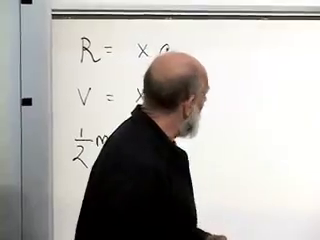
\includegraphics[width=0.72\textwidth]{lecture_09_figure_02.png}
  \caption{Плоская расширяющаяся метрика, в которой масштабный фактор умножает
  евклидов пространственный элемент длины. Исходный кадр: 00:09:12.}
  \label{fig:l09-expanding-metric-board}
\end{figure}

Представьте себе координаты, нанесённые на резиновый лист. Координатные метки остаются
прикреплёнными к листу, тогда как физическое расстояние между ними растёт. Поэтому такая
разность координат, как «от \(x=0\) до \(x=1\)», — это лишь пара меток. Расстояние,
представляемое этим интервалом, равно \(a(t)\). Найти уравнение, управляющее этим
масштабным фактором, — и есть динамическая задача лекции.

\section{Замкнутая, плоская и открытая пространственные геометрии}

Плоскостность — это наблюдательное упрощение, а не следствие
однородности. Существуют три однородные и изотропные пространственные геометрии:
с положительной, нулевой и отрицательной кривизной. Чтобы понять случай
положительной кривизны, полезно быть точным в отношении размерности.

Геометрическое место точек
\begin{equation}
  X_1^2+X_2^2=R^2
\end{equation}
есть окружность, или одномерная сфера \(S^1\). Её заполненная внутренняя область — это диск, который также называют
двумерным шаром. Добавление ещё одной координаты вложения даёт
\begin{equation}
  X_1^2+X_2^2+X_3^2=R^2,
\end{equation}
обычную двумерную сферу \(S^2\). Добавление четвёртой координаты вложения даёт
\begin{equation}
  X_1^2+X_2^2+X_3^2+X_4^2=R^2,
  \label{eq:l09-three-sphere}
\end{equation}
трёхсферу \(S^3\), которая сама является трёхмерным пространством. Мы не можем
наглядно представить её четырёхмерное вложение, но внутренняя геометрия не нуждается
в таком вложении, чтобы существовать.

\begin{figure}[H]
  \centering
  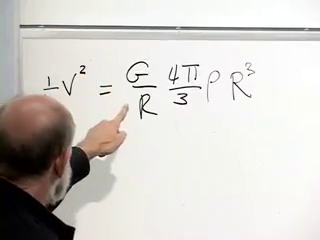
\includegraphics[width=0.72\textwidth]{lecture_09_figure_03.png}
  \caption{Уравнение вложения, используемое для введения трёхсферы. Исходный
  кадр: 00:16:40.}
  \label{fig:l09-three-sphere-board}
\end{figure}

Каждая точка идеальной сферы геометрически эквивалентна любой другой,
и любое направление в точке эквивалентно любому другому. Поэтому сфера и
однородна, и изотропна. Если её радиус умножить на \(a(t)\), всё
пространство расширяется или сжимается, не выделяя никакого центра на самой сфере. Прослеживание
такой Вселенной назад во времени не помещает всю материю в одно особое место
во внешней пустоте. Малым становится всё пространство, поэтому любая пара точек
оказывается близкой. Большой взрыв — не взрыв из одной точки пространства.

На сфере положительной кривизны сумма углов геодезических треугольников больше
\(180^\circ\). У плоских треугольников сумма углов в точности равна \(180^\circ\). В
однородной геометрии отрицательной кривизны, лишь приблизительно изображаемой седлом,
сумма углов меньше \(180^\circ\). Эти внутренние критерии различают
три случая.

\begin{figure}[H]
  \centering
  \includegraphics[width=0.72\textwidth]{lecture_09_figure_07.png}
  \caption{Положительная, нулевая и отрицательная кривизна, схематически показанные через их
  характерные формы треугольников. Исходный кадр: 00:37:30.}
  \label{fig:l09-curvature-board}
\end{figure}

Совершенно плоская локальная метрика сама по себе не доказывает, что пространство
топологически бесконечно. Компактные плоские топологии математически возможны,
хотя в лекции принимается простейшая бесконечная евклидова модель.
\editorialnote{Эта оговорка о глобальной топологии не требуется для всей
последующей локальной динамики.}

\section{Сопутствующие метки и закон Хаббла}

Теперь вернёмся к расширяющемуся плоскому листу и нанесём на него координатную сетку. В
сопутствующих координатах сетка расширяется вместе с крупномасштабным потоком материи. Галактика,
или, точнее, достаточно грубо усреднённое скопление галактик,
сохраняет приблизительно фиксированную координатную метку, хотя её физическое
расстояние до другого сопутствующего объекта меняется.

\begin{figure}[H]
  \centering
  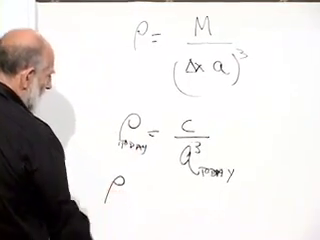
\includegraphics[width=0.72\textwidth]{lecture_09_figure_04.png}
  \caption{Координатная сетка, увлекаемая расширяющимся пространственным листом.
  Исходный кадр: 00:22:20.}
  \label{fig:l09-comoving-grid-board}
\end{figure}

Для двух объектов, разделённых вдоль оси \(x\) фиксированным сопутствующим интервалом
\(\Delta x\), физическое расстояние между ними равно
\begin{equation}
  D(t)=a(t)\,\Delta x.
  \label{eq:l09-physical-distance}
\end{equation}
Дифференцируя при фиксированном \(\Delta x\), получаем
\begin{equation}
  v(t)=\dot a(t)\,\Delta x
      =\frac{\dot a(t)}{a(t)}D(t).
\end{equation}
Введя определение
\begin{equation}
  H(t)\equiv\frac{\dot a(t)}{a(t)},
  \label{eq:l09-hubble-parameter}
\end{equation}
получаем закон Хаббла,
\begin{equation}
  v=H(t)D.
  \label{eq:l09-hubble-law}
\end{equation}
Слово «постоянная» в выражении «постоянная Хаббла» означает постоянство в
пространстве при заданном космическом времени. Оно не подразумевает постоянства
на протяжении космической истории.

\begin{figure}[H]
  \centering
  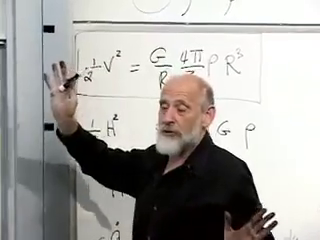
\includegraphics[width=0.72\textwidth]{lecture_09_figure_05.png}
  \caption{Вывод на доске: \(D=a\Delta x\),
  \(v=(\dot a/a)D=HD\). Исходный кадр: 00:26:40.}
  \label{fig:l09-hubble-board}
\end{figure}

\begin{classroomqa}
\audiencequestion{Если далёкая галактика наблюдается в более ранний момент
времени, должен ли выведенный для неё параметр Хаббла действительно совпадать со
значением, измеренным сегодня поблизости?}
\lecturerresponse{Только когда время, на которое мы заглядываем в прошлое,
мало по сравнению с возрастом Вселенной. На умеренных расстояниях \(H(t)\) меняется настолько
мало, что полезно пользоваться одним числом. На по-настоящему космологических расстояниях мы видим
более ранние эпохи, и зависимость \(a\) и \(H\) от времени необходимо учитывать. Это одна из причин, по которым нам
нужно динамическое уравнение для масштабного фактора.}
\end{classroomqa}

\section{Нулевые лучи в расширяющейся системе координат}

\begin{classroomqa}
\audiencequestion{Влияет ли масштабный фактор на распространение света
между далёкими галактиками?}
\lecturerresponse{Световой луч идёт по нулевой траектории, поэтому \(d\tau=0\). Для
луча, движущегося вдоль положительного направления оси \(x\), \(dy=dz=0\), и расширяющаяся метрика
даёт
\begin{align}
  0&=dt^2-a^2(t)dx^2,
  &dt&=a(t)dx,\notag\\
  &&\frac{dx}{dt}&=\frac{1}{a(t)}.
  \label{eq:l09-null-ray}
\end{align}
Координатная скорость убывает по мере роста \(a(t)\), однако локальная физическая скорость
света остаётся \(c=1\). Фиксированный координатный интервал соответствует
увеличивающемуся физическому расстоянию.}
\end{classroomqa}

\begin{figure}[H]
  \centering
  \includegraphics[width=0.72\textwidth]{lecture_09_figure_06.png}
  \caption{Нулевое условие и \(dt=a(t)dx\) для радиального распространения света.
  Исходный кадр: 00:30:54.}
  \label{fig:l09-null-board}
\end{figure}

Можно выбрать координаты, в которых тот же факт формулируется как «свет замедляется
вдали», но тогда длины и часы приходится описывать столь же неудобным
образом. Язык расширяющегося пространства чище, потому что сохраняет
локальное утверждение о том, что каждый свободно падающий наблюдатель измеряет одну и ту же
скорость света.

\begin{classroomqa}
\audiencequestion{Есть ли свидетельства того, что локальное распространение света и атомная
физика одинаковы в далёких галактиках?}
\lecturerresponse{Операциональный смысл имеют только безразмерные сравнения.
Выберите атомный размер в качестве единицы длины и атомный или ядерный
период в качестве единицы времени, а затем спросите, сколько таких периодов свету требуется,
чтобы пройти выбранную длину. Спектральные наблюдения подтверждают утверждение,
что эти безразмерные отношения одинаковы в удалённых областях. Свидетельства косвенны,
но именно такого рода сравнениями и проверяют однородность локальных законов.}
\end{classroomqa}

Когда наблюдаемая Вселенная была чрезвычайно мала, свет мог быстро пересечь данную физическую область за соответствующее время ее прохождения светом. Это не означает, что \(c\) было иным. Это означает, что мала была сама область.

\section{Ньютоновская сфера внутри Вселенной}

Теперь перейдем от кинематики к динамике. Поместим себя в начало координат и построим сферу, достаточно большую, чтобы в ней содержалось много галактик и скоплений. Выберем галактику на ее границе. В однородной Вселенной распределение массы сферически симметрично относительно нас, и теорема Ньютона об оболочке дает два решающих факта:
\begin{enumerate}
  \item все сферически распределенное вещество вне выбранного радиуса оказывает на граничную галактику нулевую суммарную ньютоновскую силу;
  \item все вещество внутри сферы действует при этом радиальном движении так, как если бы оно было сосредоточено в центре.
\end{enumerate}
Мы используем систему отсчета, в которой покоимся, поэтому скорости и ускорения в следующем рассуждении измеряются относительно нас.

\begin{figure}[H]
  \centering
  \includegraphics[width=0.72\textwidth]{lecture_09_figure_08.png}
  \caption{Построение по теореме об оболочке: мы в центре, а пробная галактика — на границе большой однородной сферы. Исходный кадр на 00:41:10.}
  \label{fig:l09-shell-board}
\end{figure}

\begin{figure}[H]
  \centering
  \begin{tikzpicture}[scale=0.92,>=Latex]
    \draw[thick] (0,0) circle (2.35);
    \fill (0,0) circle (2pt) node[below left] {us};
    \fill (2.35,0) circle (2.2pt) node[right] {test galaxy \(m\)};
    \draw[->,thick,blue!65!black] (0.18,0) -- (2.15,0)
      node[midway,above] {\(R=a(t)x\)};
    \draw[->,thick,red!65!black] (2.35,0.12) -- (3.25,0.12)
      node[midway,above] {\(v=\dot a(t)x\)};
    \node[align=center,text width=7cm] at (0,-2.85)
      {outside shells cancel;\\enclosed mass acts at the center};
  \end{tikzpicture}
  \caption{Аккуратная реконструкция ньютоновского построения.}
  \label{fig:l09-shell-clean}
\end{figure}

Если у галактики фиксированная сопутствующая координата \(x\), то ее физический радиус и скорость равны
\begin{equation}
  R(t)=x a(t),
  \qquad
  v(t)=x\dot a(t)=H(t)R(t).
  \label{eq:l09-radius-velocity}
\end{equation}
Пусть \(M\) — масса, заключенная внутри сферы, а \(m\) — масса пробной галактики. Тогда ньютоновская энергия равна
\begin{equation}
  E=\frac12 m v^2-\frac{GMm}{R}.
  \label{eq:l09-newtonian-energy}
\end{equation}

\begin{figure}[H]
  \centering
  \includegraphics[width=0.72\textwidth]{lecture_09_figure_09.png}
  \caption{Полная последовательность записей на доске: \(R=xa\), \(v=x\dot a\) и уравнение ньютоновской энергии в случае \(E=0\). Исходный кадр на 00:48:40.}
  \label{fig:l09-energy-board}
\end{figure}

Энергия может быть положительной, нулевой или отрицательной. Начнем с границы между уходом на бесконечность и реколлапсом, \(E=0\), для которой
\begin{equation}
  \frac12 v^2=\frac{GM}{R}.
  \label{eq:l09-zero-energy}
\end{equation}

\begin{classroomqa}
\audiencequestion{Что означает нулевая полная энергия для удаляющейся галактики?}
\lecturerresponse{Это в точности случай скорости убегания. Положительная энергия означает движение со скоростью выше скорости убегания; отрицательная энергия означает движение со скоростью ниже скорости убегания и, в ньютоновской картине, содержащей только вещество, в конечном итоге возвращение. Мы начинаем с границы между этими возможностями и вернемся к другим знакам после вывода уравнения для плоского случая.}
\end{classroomqa}

\begin{classroomqa}
\audiencequestion{Меняется ли заключенная масса \(M\) по мере расширения сферы?}
\lecturerresponse{Нет. Это сопутствующая сфера, так что внутри нее остаются одни и те же частицы. Ее физический объем растет, а плотность падает, но полная масса внутри нее остается постоянной. Это различие между \(M\) и \(\rho(t)\) существенно.}
\end{classroomqa}

Для однородной плотности \(\rho(t)\),
\begin{equation}
  M=\frac{4\pi}{3}\rho(t)R^3.
  \label{eq:l09-enclosed-mass}
\end{equation}
Подстановка в \eqref{eq:l09-zero-energy} дает
\begin{equation}
  \frac12 v^2
  =\frac{G}{R}\left(\frac{4\pi}{3}\rho R^3\right).
  \label{eq:l09-enclosed-energy}
\end{equation}

\begin{figure}[H]
  \centering
  \includegraphics[width=0.72\textwidth]{lecture_09_figure_10.png}
  \caption{Подстановка заключенной массы в уравнение нулевой энергии. Исходный кадр на 00:54:16.060.}
  \label{fig:l09-enclosed-mass-board}
\end{figure}

Используя \(v=HR\), находим
\begin{align}
  \frac12 H^2R^2
    &=\frac{4\pi G}{3}\rho R^2,\\
  H^2
    &=\frac{8\pi G}{3}\rho.
\end{align}
Следовательно, закон расширения при нулевой энергии для пространственно плоского случая имеет вид
\begin{equation}
  \boxed{\left(\frac{\dot a}{a}\right)^2
  =\frac{8\pi G}{3}\rho(t)}.
  \label{eq:l09-flat-friedmann}
\end{equation}
Сокращение \(R^2\) не случайно. Однородная Вселенная должна давать одно и то же \(H(t)\) независимо от того, какая сопутствующая галактика была выбрана в качестве пробного объекта.

\begin{figure}[H]
  \centering
  \includegraphics[width=0.72\textwidth]{lecture_09_figure_11.png}
  \caption{Сокращение радиуса и получающееся на доске соотношение Фридмана для плоского случая. Исходный кадр на 00:57:30.}
  \label{fig:l09-friedmann-board}
\end{figure}

\begin{classroomqa}
\audiencequestion{Есть ли свидетельства в пользу соотношения для нулевой энергии?}
\lecturerresponse{Обе стороны можно определить из наблюдений: \(H\) — по данным о разбегании, а \(\rho\) — учитывая звезды, газ, темную материю и энергию вакуума. Сравнение, приведенное в лекции, показало согласие двух сторон с точностью порядка процента. Эта оговорка важна: нужно включить все формы энергии, а более позднее обсуждение энергии вакуума меняет наивную интерпретацию через скорость убегания.}
\end{classroomqa}

В единицах \(c=1\) плотность массы и плотность энергии имеют одинаковые размерности. Поэтому символ \(\rho\) будет обозначать полную плотность энергии, соответствующую обсуждаемой компоненте.

\section{Обычное вещество и закон двух третей}

Уравнение \eqref{eq:l09-flat-friedmann} не замкнуто, пока мы не знаем, как меняется \(\rho(t)\). Сначала заполним сопутствующий прямоугольный ящик медленно движущимися нерелятивистскими частицами. Его координатные размеры фиксированы, тогда как его физический объем растет как
\begin{equation}
  V(t)=a^3(t)\,\Delta x\,\Delta y\,\Delta z.
\end{equation}
Число частиц и суммарная масса покоя в ящике остаются постоянными, поэтому
\begin{equation}
  \rho_{\mathrm m}(t)=\frac{C_{\mathrm m}}{a^3(t)}.
  \label{eq:l09-matter-dilution}
\end{equation}
Нормируя к современной эпохе \(t_0\),
\begin{equation}
  \frac{\rho_{\mathrm m}(t)}{\rho_{\mathrm m,0}}
  =\left(\frac{a_0}{a(t)}\right)^3.
  \label{eq:l09-matter-normalized}
\end{equation}

\begin{figure}[H]
  \centering
  \includegraphics[width=0.72\textwidth]{lecture_09_figure_12.png}
  \caption{Плотность вещества, ее разбавление по закону \(a^{-3}\) и нормировка на современную эпоху. Исходный кадр на 01:04:47.940.}
  \label{fig:l09-density-board}
\end{figure}

\begin{classroomqa}
\audiencequestion{Какова грубая современная плотность энергии Вселенной и могут ли одни обычные атомы ее обеспечить?}
\lecturerresponse{Подсчет видимой барионной материи дает лишь часть ответа. Темная материя и темная энергия тоже должны быть представлены как эквивалентная масса-энергия. В лекции приводится грубая шкала — от одного атома до нескольких десятков эквивалентов массы водорода на кубический метр, — с акцентом на порядок величины, а не на точную инвентаризацию.}
\end{classroomqa}

Подставим \eqref{eq:l09-matter-dilution} в \eqref{eq:l09-flat-friedmann} и соберем все не зависящие от времени множители в положительную константу \(C\):
\begin{equation}
  \left(\frac{\dot a}{a}\right)^2=\frac{C}{a^3},
  \qquad
  \dot a^2=\frac{C}{a}.
  \label{eq:l09-matter-ode}
\end{equation}
Есть два наглядных способа решить это уравнение. Степенной анзац \(a=K t^p\) требует
\begin{equation}
  p-1=-\frac{p}{2},
  \qquad p=\frac23.
\end{equation}
Эквивалентно можно выбрать ветвь квадратного корня, отвечающую расширению, и проинтегрировать:
\begin{equation}
  a^{1/2}\frac{da}{dt}=\sqrt C,
  \qquad
  \int a^{1/2}da=\sqrt C\int dt,
\end{equation}
поэтому после выбора Большого взрыва в качестве начала отсчета времени
\begin{equation}
  a^{3/2}\propto t,
  \qquad
  \boxed{a(t)\propto t^{2/3}}.
  \label{eq:l09-matter-solution}
\end{equation}
При выводе у доски на мгновение теряется множитель при сопоставлении коэффициентов, затем рассуждение возвращается к интегралу и проверяет показатель. В конспекте эта проверка сохранена, но выписана только исправленная алгебра.

\begin{figure}[H]
  \centering
  \includegraphics[width=0.72\textwidth]{lecture_09_figure_13.png}
  \caption{Степенной анзац и выделенный рамкой показатель \(p=2/3\). Исходный кадр на 01:13:05.}
  \label{fig:l09-matter-solution-board}
\end{figure}

Дифференцируя решение, получаем
\begin{equation}
  H(t)=\frac{\dot a}{a}=\frac{2}{3t}.
  \label{eq:l09-matter-hubble}
\end{equation}
Параметр Хаббла в прошлом был больше. Следовательно, если смотреть достаточно далеко, чтобы время взгляда назад было заметным, не следует без изменения экстраполировать локальное линейное соотношение, используя сегодняшнее \(H_0\).

\begin{figure}[H]
  \centering
  \includegraphics[width=0.72\textwidth]{lecture_09_figure_14.png}
  \caption{Вычисление \(\dot a/a\) для \(a\propto t^{2/3}\) дает \(H=2/(3t)\). Исходный кадр на 01:20:42.}
  \label{fig:l09-hubble-time-board}
\end{figure}

\section{Знак энергии и пространственная кривизна}

Ньютоновское рассуждение провело нас через плоский случай с нулевой энергией. Общая теория относительности добавляет факт, который нельзя получить из одной лишь теоремы об оболочке: знак удельной энергии ньютоновского типа соответствует знаку пространственной кривизны.
\begin{center}
\begin{tabular}{@{}>{\raggedright\arraybackslash}p{0.20\linewidth}
                    >{\raggedright\arraybackslash}p{0.29\linewidth}
                    >{\raggedright\arraybackslash}p{0.37\linewidth}@{}}
  \toprule
  Полная энергия & Пространственная кривизна & Судьба в модели только с веществом \\
  \midrule
  положи\-тельная & отрицательная (открытая) & расширяется вечно \\
  нулевая & нулевая (плоская) & приближается к границе убегания \\
  отри\-цательная & положительная (замкнутая) & расширяется, разворачивается, реколлапсирует \\
  \bottomrule
\end{tabular}
\end{center}
Последний столбец предполагает отсутствие энергии вакуума. В аналогии со снарядом положительная энергия означает скорость выше скорости убегания, нулевая — точно скорость убегания, а отрицательная — скорость ниже скорости убегания. Уравнения Эйнштейна отождествляют эти три случая соответственно с открытой, плоской и замкнутой пространственной геометрией.

\section{Фотоны и закон одной второй}

Закон для вещества \(\rho\propto a^{-3}\) предполагает, что энергия каждой частицы приблизительно постоянна, тогда как численная плотность падает. Фотоны нарушают это предположение. Для фотона,
\begin{equation}
  E=h\nu=\frac{hc}{\lambda}.
\end{equation}
Расширение растягивает его длину волны пропорционально масштабному фактору,
\begin{equation}
  \lambda\propto a,
  \qquad E\propto a^{-1}.
\end{equation}
Численная плотность фотонов по-прежнему убывает как \(a^{-3}\), а энергия каждого фотона дает еще один множитель \(a^{-1}\). Поэтому
\begin{equation}
  \boxed{\rho_{\mathrm r}(t)\propto a^{-4}(t)}.
  \label{eq:l09-radiation-dilution}
\end{equation}

Аналогия с гитарной струной хорошо передает физическую картину. Если щипнуть струну, а затем удлинить ее колеблющуюся часть, длина волны увеличится, а тон понизится. Мода фотона в расширяющемся сопутствующем ящике ведет себя аналогично. Если мысленно прокрутить картину назад, сжатие укорачивает длины волн и повышает энергии фотонов.

\begin{figure}[H]
  \centering
  \includegraphics[width=0.72\textwidth]{lecture_09_figure_15.png}
  \caption{Соотношение для плотности вещества, обобщенное на доске до закона масштабирования излучения \(\rho_{\mathrm r}\propto a^{-4}\). Исходный кадр на 01:29:20.}
  \label{fig:l09-radiation-board}
\end{figure}

Подстановка \(\rho_{\mathrm r}\propto a^{-4}\) в плоское уравнение Фридмана дает
\begin{equation}
  \left(\frac{\dot a}{a}\right)^2=\frac{C_{\mathrm r}}{a^4},
  \qquad
  \dot a\propto a^{-1},
\end{equation}
и, следовательно,
\begin{equation}
  \boxed{a(t)\propto t^{1/2}}.
  \label{eq:l09-radiation-solution}
\end{equation}
Это растет медленнее, чем \(t^{2/3}\). Достаточно далеко в прошлом излучение
должно доминировать над обычным веществом, потому что \(a^{-4}\) растет быстрее,
чем \(a^{-3}\), при уменьшении \(a\). В лекции переход между доминированием вещества и излучения относится примерно к эпохе, когда масштабный фактор был приблизительно в тысячу раз меньше, чем сегодня. До этого перехода во Вселенной доминировало излучение; после него, в течение долгого интервала, в ней доминировало вещество.

\section{Энергия вакуума и экспоненциальное расширение}

Для энергии вакуума зависимость от масштабного фактора противоположна. Ее плотность является свойством пустого пространства и не разрежается при расширении Вселенной:
\begin{equation}
  \rho_\Lambda=\text{constant}.
  \label{eq:l09-vacuum-density}
\end{equation}
Плотности обычного вещества и излучения при движении в прошлое возрастают, тогда как этот член — нет. Поэтому в ранней Вселенной он был менее важен, а по мере разрежения остальных компонент становится более важным. В лекции используется тогдашняя оценка, согласно которой на энергию вакуума приходится около \(70\%\) современной космической плотности энергии.

При постоянной \(\rho_\Lambda\) уравнение \eqref{eq:l09-flat-friedmann} дает
постоянный темп расширения
\begin{equation}
  H_\Lambda=\sqrt{\frac{8\pi G}{3}\rho_\Lambda},
  \qquad
  \frac{\dot a}{a}=H_\Lambda.
\end{equation}
Следовательно,
\begin{equation}
  \boxed{a(t)=a(t_i)e^{H_\Lambda(t-t_i)}}.
  \label{eq:l09-vacuum-solution}
\end{equation}

\begin{figure}[H]
  \centering
  \includegraphics[width=0.72\textwidth]{lecture_09_figure_16.png}
  \caption{Уравнение с постоянной плотностью, приводящее к экспоненциальному расширению.
  Исходный кадр: 01:35:48.}
  \label{fig:l09-vacuum-board}
\end{figure}

В том наблюдаемом масштабе, о котором говорилось в лекции, линейный размер Вселенной удваивается примерно за десять-двенадцать миллиардов лет. Происхождение этой малой, но ненулевой плотности вакуума остается необъясненным; ее существование и ее влияние на расширение — эмпирические факты.

\begin{classroomqa}
\audiencequestion{Является ли энергия вакуума в этом обсуждении тем же самым, что и тёмная энергия?}
\lecturerresponse{Да. Здесь «тёмная энергия» обозначает постоянную плотность энергии вакуума, то есть космологическую постоянную. Можно вообразить и более общие зависящие от времени модели тёмной энергии, но в вычисления этой лекции они не входят.}
\end{classroomqa}

\section{Как расширяющаяся Вселенная вызывает красное смещение света}

\begin{classroomqa}
\audiencequestion{Как фотоны могут знать, что мы выбрали расширяющиеся сопутствующие
координаты, и поэтому уменьшать свою энергию?}
\lecturerresponse{Никак: на наши обозначения они не реагируют. Они распространяются в
геометрии, в которой физические расстояния меняются. Волновой цуг,
занимающий область, физический размер которой удваивается, приобретает
удвоенную длину волны. Сопутствующие координаты лишь экономно описывают это
растяжение; они его не вызывают.}
\end{classroomqa}

\begin{classroomqa}
\audiencequestion{Откуда приходят фоновые фотоны, достигающие нас сегодня?}
\lecturerresponse{Смотреть дальше — значит смотреть в более ранние времена. В конце
концов мы видим эпоху, когда космическое вещество было ионизованной плазмой,
непрозрачной, потому что фотоны многократно рассеивались на свободных
заряженных частицах. Граница, с которой фотоны в последний раз могли
свободно дойти до нас, выглядит как сфера, окружающая наблюдателя:
поверхность последнего рассеяния.}
\end{classroomqa}

\begin{figure}[H]
  \centering
  \includegraphics[width=0.72\textwidth]{lecture_09_figure_17.png}
  \caption{Схема поверхности последнего рассеяния с центром в наблюдателе и
  все более удаленных оболочек. Исходный кадр: 01:42:05.}
  \label{fig:l09-last-scattering-board}
\end{figure}

\begin{figure}[H]
  \centering
  \begin{tikzpicture}[scale=0.9,>=Latex]
    \fill (0,0) circle (2pt) node[below] {observer};
    \draw[thick,orange!70!black] (0,0) circle (2.55);
    \node[orange!70!black,align=center] at (0,3.05)
      {surface of last scattering};
    \foreach \a in {25,75,145,210,285,335}{
      \draw[->,blue!60!black] ({2.55*cos(\a)},{2.55*sin(\a)}) --
        ({1.7*cos(\a)},{1.7*sin(\a)});
    }
    \draw[decorate,decoration={snake,amplitude=1.5pt,segment length=7pt},
      red!65!black,thick,->] (-2.5,0) -- (-0.15,0);
    \node[red!65!black,below] at (-1.35,-0.15)
      {redshifted photon};
  \end{tikzpicture}
  \caption{Аккуратная реконструкция картины последнего рассеяния.}
  \label{fig:l09-last-scattering-clean}
\end{figure}

Излучение было испущено со спектром, характерным для горячей плазмы, и
приходит к нам с длинами волн примерно в тысячу раз большими. На
доплеровском языке лекции далекая излучающая поверхность быстро удаляется, и
ее излучение сильно смещено в красную сторону. На геометрическом языке волна
растягивается при распространении. Обе картины выражают одно и то же
соотношение,
\begin{equation}
  1+z=\frac{\lambda_0}{\lambda_{\mathrm{em}}}
      =\frac{a_0}{a_{\mathrm{em}}}.
  \label{eq:l09-cosmological-redshift}
\end{equation}
\editorialnote{Уравнение \eqref{eq:l09-cosmological-redshift} — стандартная количественная форма
лекционных описаний через растяжение и доплеровский эффект.}

В более раннюю эпоху наблюдения в соответствующей картине сфера
последнего рассеяния находилась бы ближе, а наблюдаемые фоновые фотоны были
бы слабее смещены в красную сторону и потому обладали бы большей энергией.
По мере течения космического времени фотоны, достигающие сопутствующего
наблюдателя от той ранней плазмы, имеют все большие длины волн.

\section{Куда девается энергия фотона при красном смещении?}

\begin{classroomqa}
\audiencequestion{Фотон испускается с энергией \(h\nu_{\mathrm{em}}\) и
приходит с красным смещением, имея меньшую энергию. Что произошло с
разностью?}
\lecturerresponse{Ньютоновский вывод начинался как уравнение энергии. Его
космологическая форма связывает темп расширения с плотностью энергии
вещества, так что энергию вещества и расширение нельзя рассматривать как
отдельно сохраняющиеся балансы. В лекции потерянная энергия фотона
описывается как переходящая в кинематический учет расширения. Аналогия с
поршнем, заполненным излучением, делает это наглядным: давление излучения
толкает поршень наружу, длины волн фотонов увеличиваются, а потерянная ими
энергия превращается в механическую работу и кинетическую энергию
поршня.}
\end{classroomqa}

\begin{figure}[H]
  \centering
  \includegraphics[width=0.72\textwidth]{lecture_09_figure_18.png}
  \caption{На доске заключенное в рамку ньютоновское уравнение энергии
  помещено над соответствующим уравнением Фридмана. Исходный кадр: 01:44:42.}
  \label{fig:l09-energy-bookkeeping-board}
\end{figure}

\begin{classroomqa}
\audiencequestion{Что связывает энергию излучения с расширением?}
\lecturerresponse{Давление. В цилиндре с подвижным поршнем фотоны
передают стенке импульс. Когда поршень движется, излучение совершает работу;
его длина волны растет, а энергия падает. В однородной расширяющейся
Вселенной буквального внешнего поршня нет, но аналогия с \(p\,dV\) объясняет,
почему плотность энергии излучения убывает быстрее, чем при одном лишь
уменьшении численной плотности.}
\end{classroomqa}

\begin{figure}[H]
  \centering
  \includegraphics[width=0.72\textwidth]{lecture_09_figure_19.png}
  \caption{Подвижный поршень, заполненный фотонами, используемый для
  наглядного представления работы давления. Исходный кадр: 01:46:40.}
  \label{fig:l09-piston-board}
\end{figure}

\begin{figure}[H]
  \centering
  \begin{tikzpicture}[scale=0.92,>=Latex]
    \draw[thick] (0,0) rectangle (5.3,2.6);
    \draw[very thick] (4.25,0) -- (4.25,2.6);
    \draw[very thick] (4.25,1.3) -- (5.25,1.3);
    \draw[->,thick,red!65!black] (5.25,1.3) -- (6.2,1.3)
      node[right] {moving piston};
    \foreach \y in {0.55,1.3,2.05}{
      \draw[decorate,decoration={snake,amplitude=1.4pt,segment length=6pt},
        blue!65!black,->] (0.35,\y) -- (3.9,\y);
    }
    \node at (2.15,-0.45) {radiation does \(p\,dV\) work};
  \end{tikzpicture}
  \caption{Аккуратная реконструкция аналогии с излучением и поршнем.}
  \label{fig:l09-piston-clean}
\end{figure}

С энергией в общей теории относительности нужно обращаться осторожно. В
общем случае в расширяющемся пространстве-времени не обязана существовать
единственная сохраняющаяся глобальная энергия, аналогичная энергии
изолированной ньютоновской системы. Локальный закон сохранения
тензора энергии-импульса, однако, остается в силе, и для однородной жидкости
он дает уравнение непрерывности
\begin{equation}
  \dot\rho+3H(\rho+p)=0,
  \label{eq:l09-continuity}
\end{equation}
которое содержит член работы давления, лежащий в основе законов
масштабирования вещества и излучения.\editorialnote{Уравнение \eqref{eq:l09-continuity} — точная локальная
релятивистская формулировка, лежащая в основе нарочито ньютоновской аналогии
с энергетическим балансом, использованной в лекции.}

Энергия вакуума делает этот парадокс особенно острым. Поскольку ее
плотность остается постоянной, тогда как объем растет, полная энергия
вакуума в сопутствующей области увеличивается. Ее отрицательное давление
входит в гравитационный источник и приводит к ускоренному расширению.
Поэтому не следует требовать отдельного сохранения наивной «энергии материи
в сопутствующей коробке», не учитывая геометрию и работу давления.

\section{Почему масштабный фактор можно убрать из временного члена}

\begin{classroomqa}
\audiencequestion{Почему масштабный фактор умножает пространственную часть
метрики, но не временную?}
\lecturerresponse{Это вопрос выбора временной координаты. Предположим, что мы
начинаем с координаты конформного времени \(t\), для которой
\begin{equation}
  d\tau^2=A^2(t)\left(dt^2-dx^2\right).
\end{equation}
Определим новое космическое время \(T\) посредством
\begin{equation}
  dT=A(t)\,dt.
\end{equation}
Тогда
\begin{equation}
  d\tau^2=dT^2-A^2\bigl(t(T)\bigr)dx^2.
\end{equation}
Общий множитель перед временным дифференциалом исчез, тогда как
физический масштабный фактор остается в пространственном члене.}
\end{classroomqa}

\begin{figure}[H]
  \centering
  \includegraphics[width=0.72\textwidth]{lecture_09_figure_20.png}
  \caption{Переопределение времени \(dT=A(t)dt\), переводящее от конформного времени к
  космическому времени. Исходный кадр: 01:51:05.}
  \label{fig:l09-time-reparam-board}
\end{figure}

\section{Кривизна, энергия вакуума и судьба Вселенной}

\begin{classroomqa}
\audiencequestion{Если бы Вселенная имела положительную кривизну, должны ли мы уже
видеть галактики, движущиеся к нам?}
\lecturerresponse{Не обязательно. Тело, запущенное со скоростью ниже скорости
убегания, сначала движется наружу, достигает точки поворота и лишь потом
падает обратно. Мы наблюдаем Вселенную в фазе расширения. Без энергии
вакуума материальная Вселенная с положительной кривизной в конечном счете
вновь сколлапсировала бы. Достаточно большая положительная энергия вакуума
предотвращает этот разворот, и наблюдаемое значение, по-видимому, достаточно
велико, чтобы в далекой перспективе сделать расширение экспоненциальным
независимо от небольшой пространственной кривизны.}
\end{classroomqa}

Экспоненциальное будущее — не энергетический рай. Звезды со временем
выгорают, плотности вещества и излучения экспоненциально падают, а далекие
области выходят за пределы причинной связи. Энергия вакуума остается, тогда
как обычные структуры становятся все более холодными и разреженными.

\begin{classroomqa}
\audiencequestion{Если заглянуть ещё дальше в прошлое, больше ли фотонов, чем обычных частиц?}
\lecturerresponse{Отношение числа фотонов к числу барионов уже огромно — по оценке, данной в лекции, примерно \(10^{10}\) фотонов на барион, — и оба этих числа в сопутствующем объёме остаются приблизительно постоянными. При переходе к более ранним временам меняется главным образом энергия, приходящаяся на фотон. Энергии фотонов растут как \(a^{-1}\), тогда как нерелятивистские массы покоя не растут. Поэтому на ранних этапах излучение доминирует по плотности энергии, хотя само это численное отношение изменяться не обязано.}
\end{classroomqa}

Главный вывод состоит в том, что одна лишь геометрия не определяет космическую историю. Плоское уравнение Фридмана задаёт связь между расширением и плотностью энергии, но временную зависимость задаёт содержимое Вселенной. Для нерелятивистской материи получается \(a\propto t^{2/3}\), для излучения — \(a\propto t^{1/2}\), а постоянная энергия вакуума даёт экспоненциальное расширение. Эти три закона упорядочивают последовательные эпохи Вселенной и объясняют, почему один и тот же масштабный фактор определяет расстояния, красные смещения и изменяющийся параметр Хаббла.

\end{document}
